%\clearpage
%\subsection{W+jets control region}

Figure
\ref{fig:CRWjetResLoosePlots1Lep}
\ref{fig:CRWjetResLoosePlots1Lep2}
\ref{fig:CRWjetResTightPlots1Lep}
\ref{fig:CRWjetResTightPlots1Lep2}
\ref{fig:CRWjetMerPlots1Lep}
\ref{fig:CRWjetMerPlots1Lep2}
show the main relevant kinematic variable distributions in the \Wjets CR in \olep channel, after \mjjtag reweighting has been applied.

\begin{figure}[ht]
    \centering
    \subfloat[]{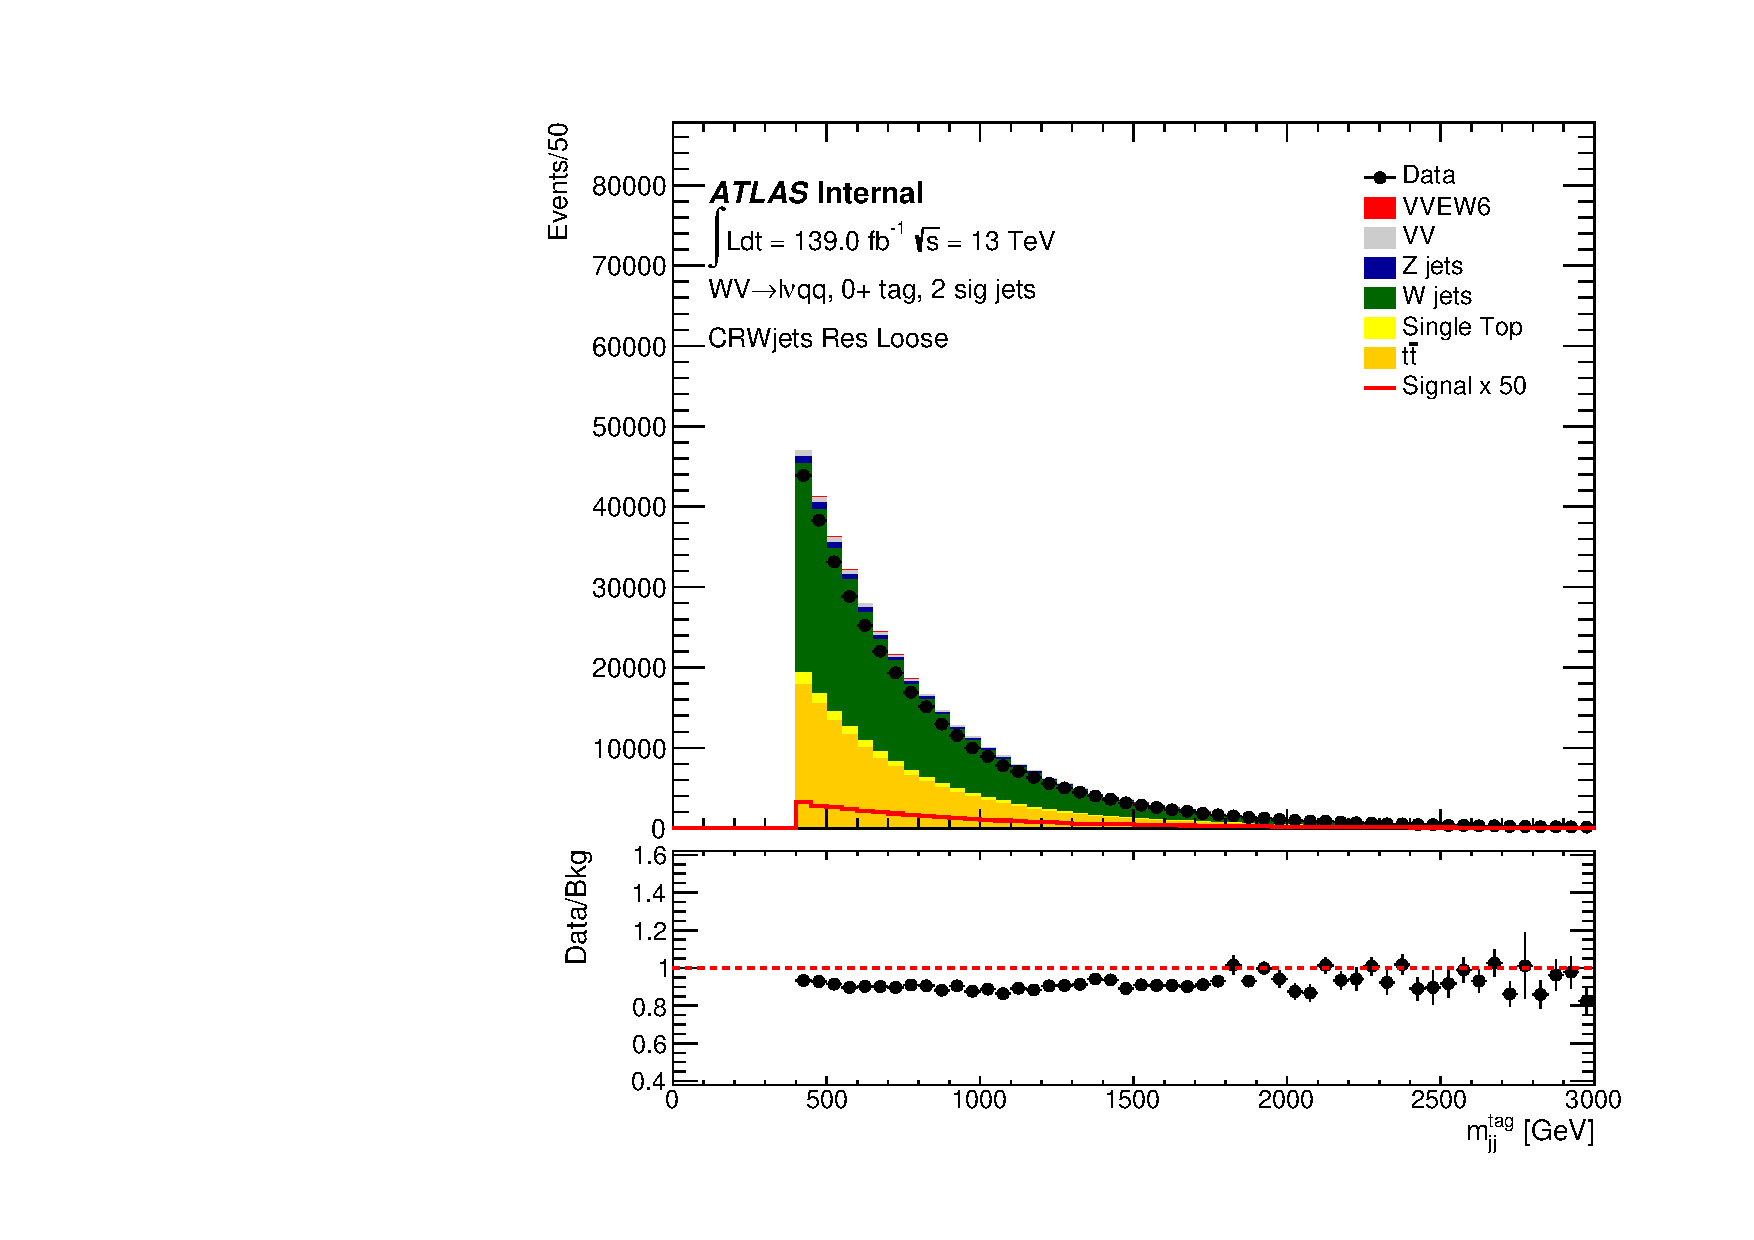
\includegraphics[width=0.3\textwidth]{figures/CRPlots/CRWjets_Res_Loose/stacked_plot_resolved_tagMjj.pdf}}
    \subfloat[]{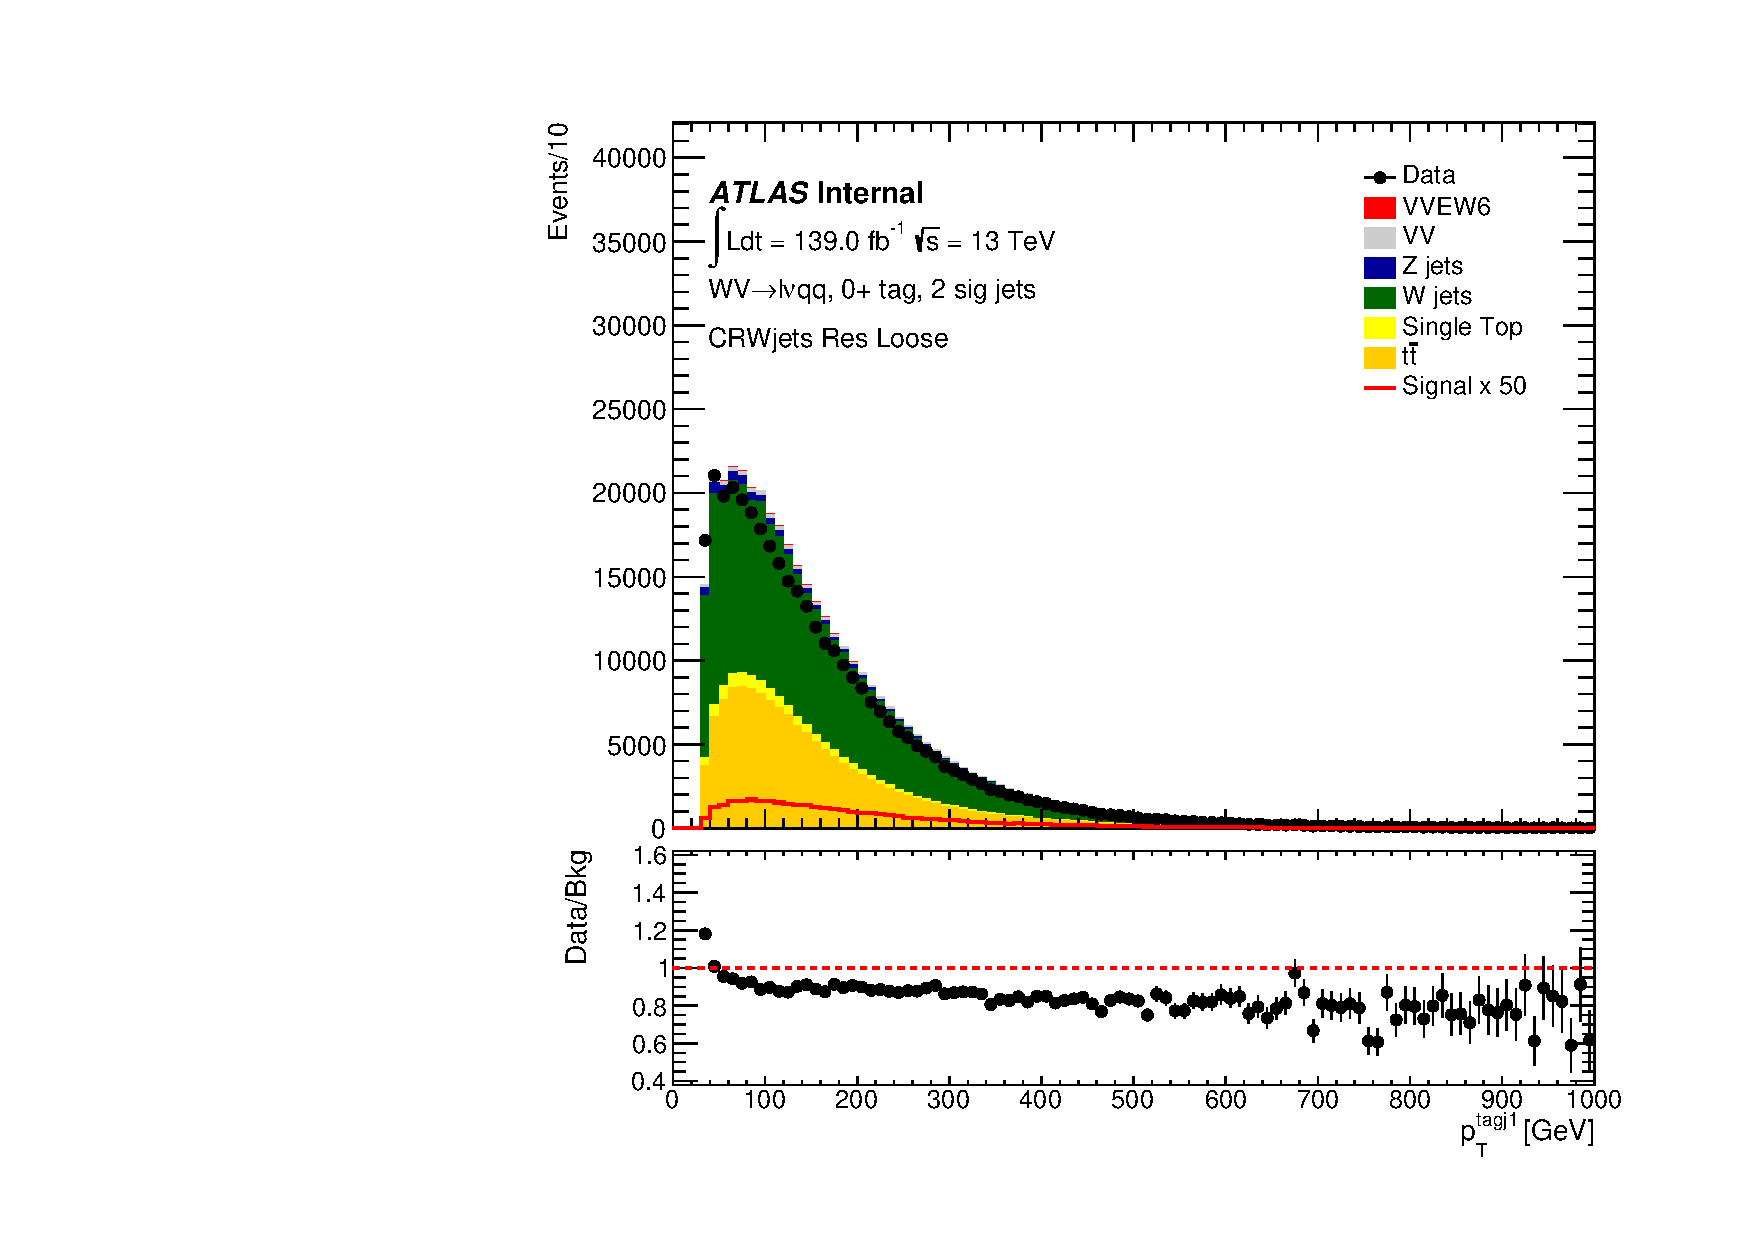
\includegraphics[width=0.3\textwidth]{figures/CRPlots/CRWjets_Res_Loose/stacked_plot_resolved_tagJ1_pt.pdf}}
    \subfloat[]{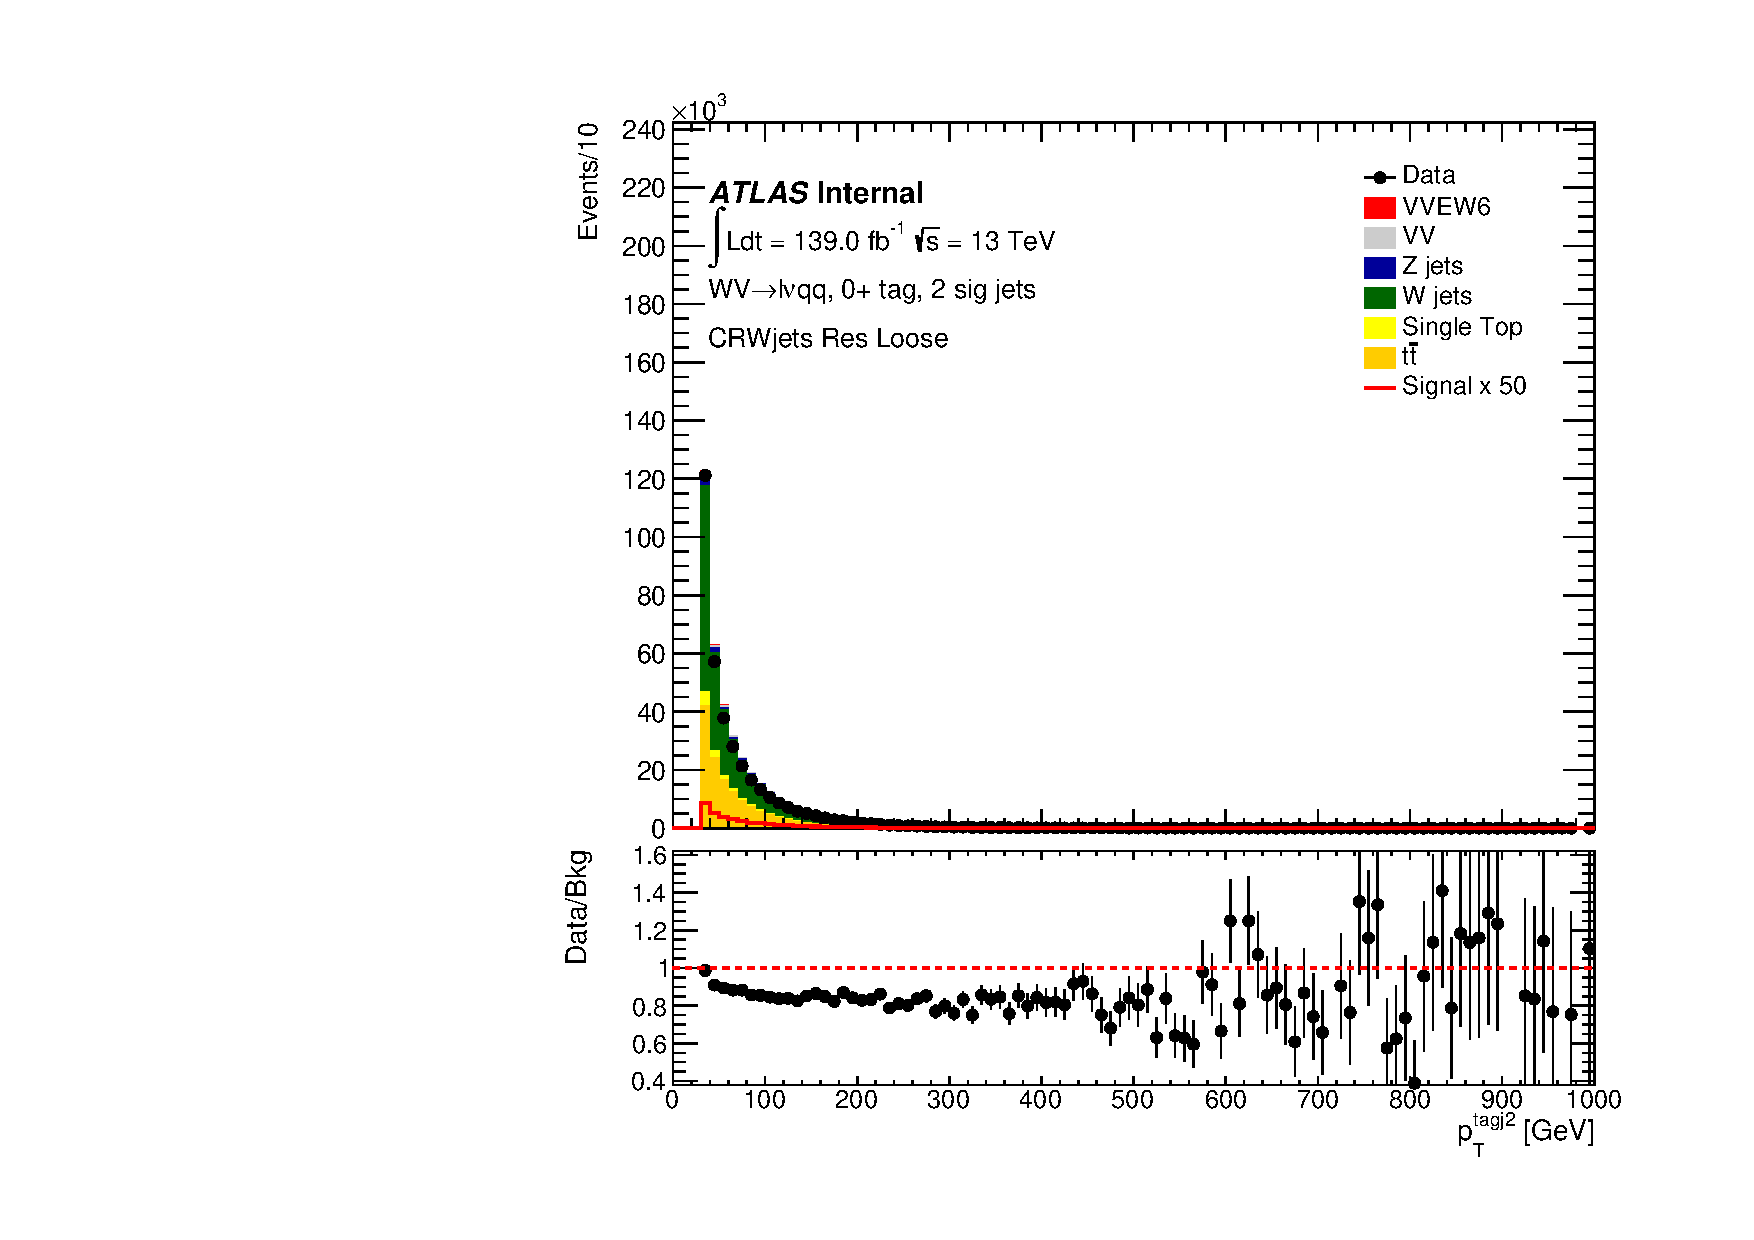
\includegraphics[width=0.3\textwidth]{figures/CRPlots/CRWjets_Res_Loose/stacked_plot_resolved_tagJ2_pt.pdf}} \\
    \subfloat[]{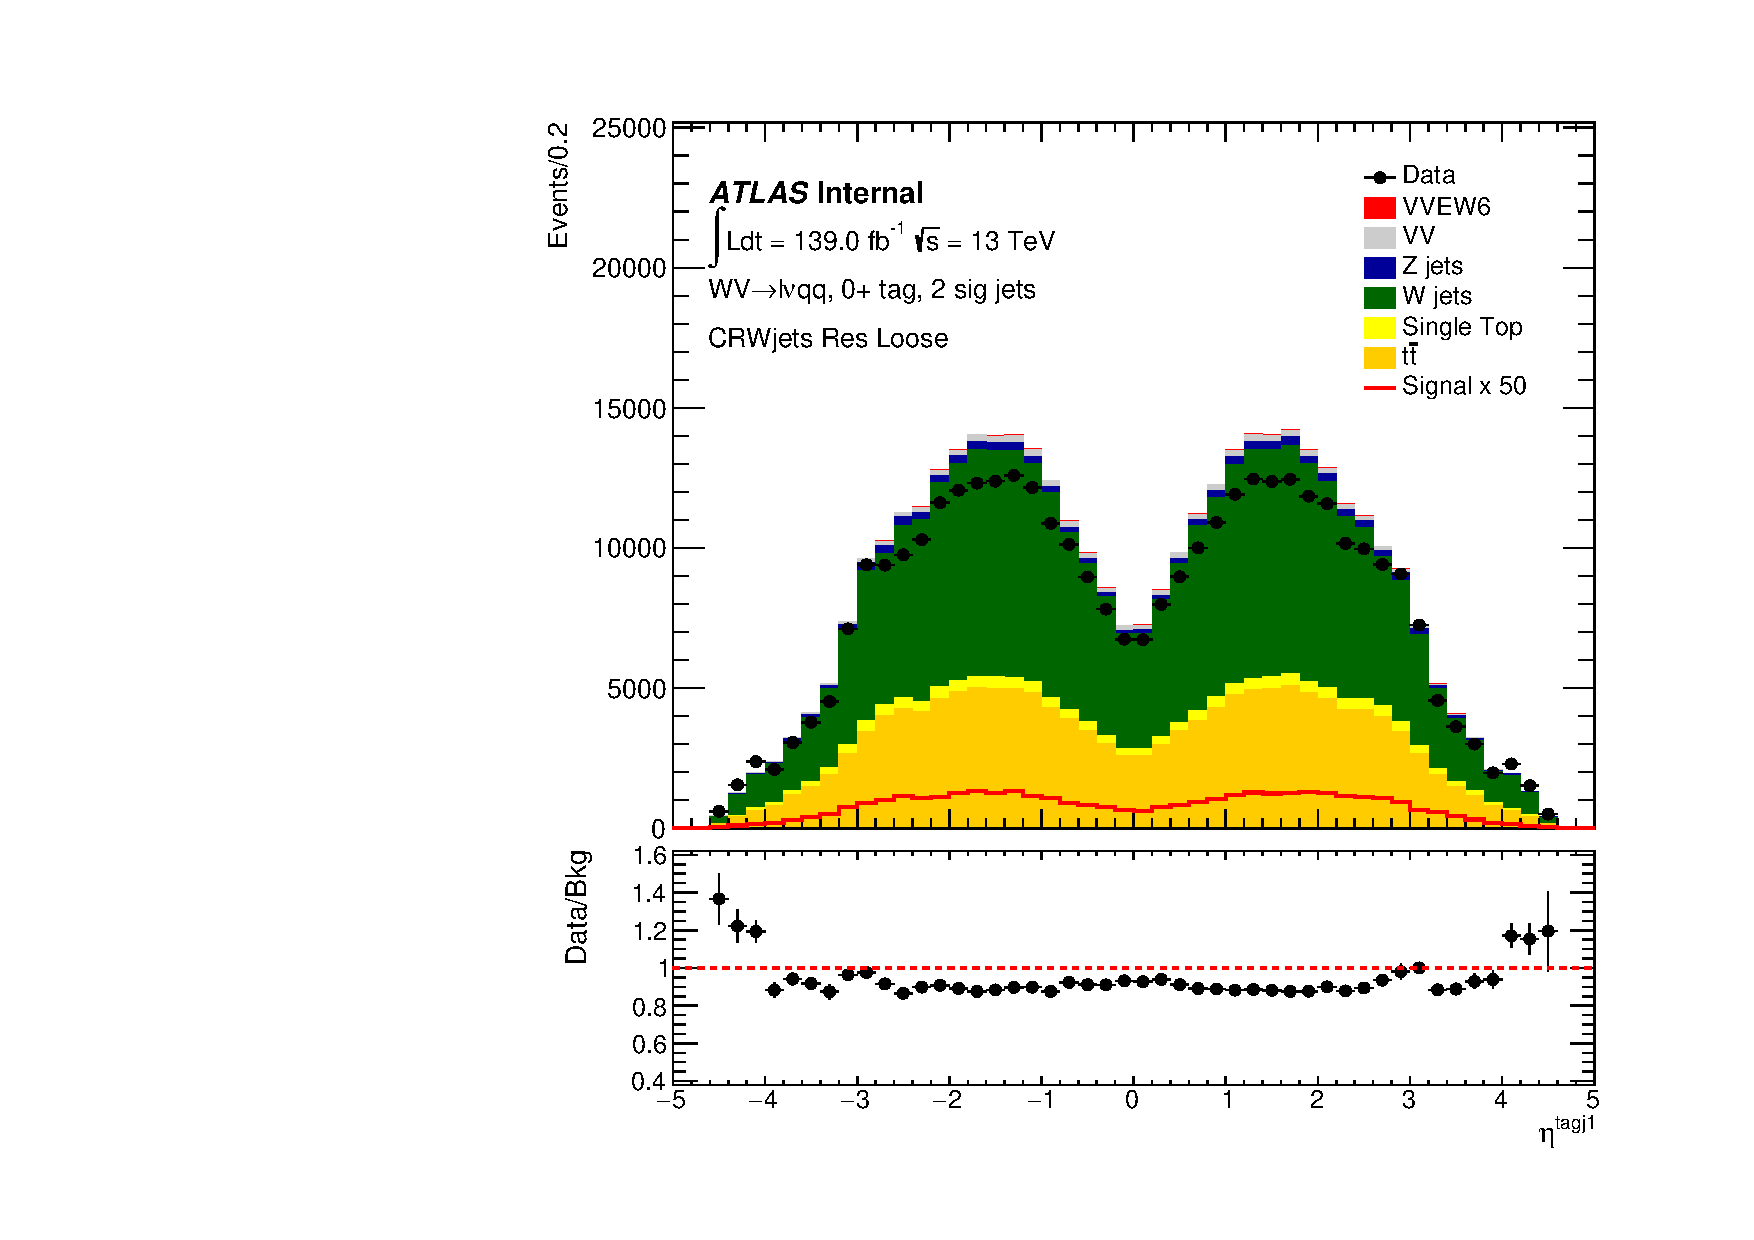
\includegraphics[width=0.3\textwidth]{figures/CRPlots/CRWjets_Res_Loose/stacked_plot_resolved_tagJ1_eta.pdf}}
    \subfloat[]{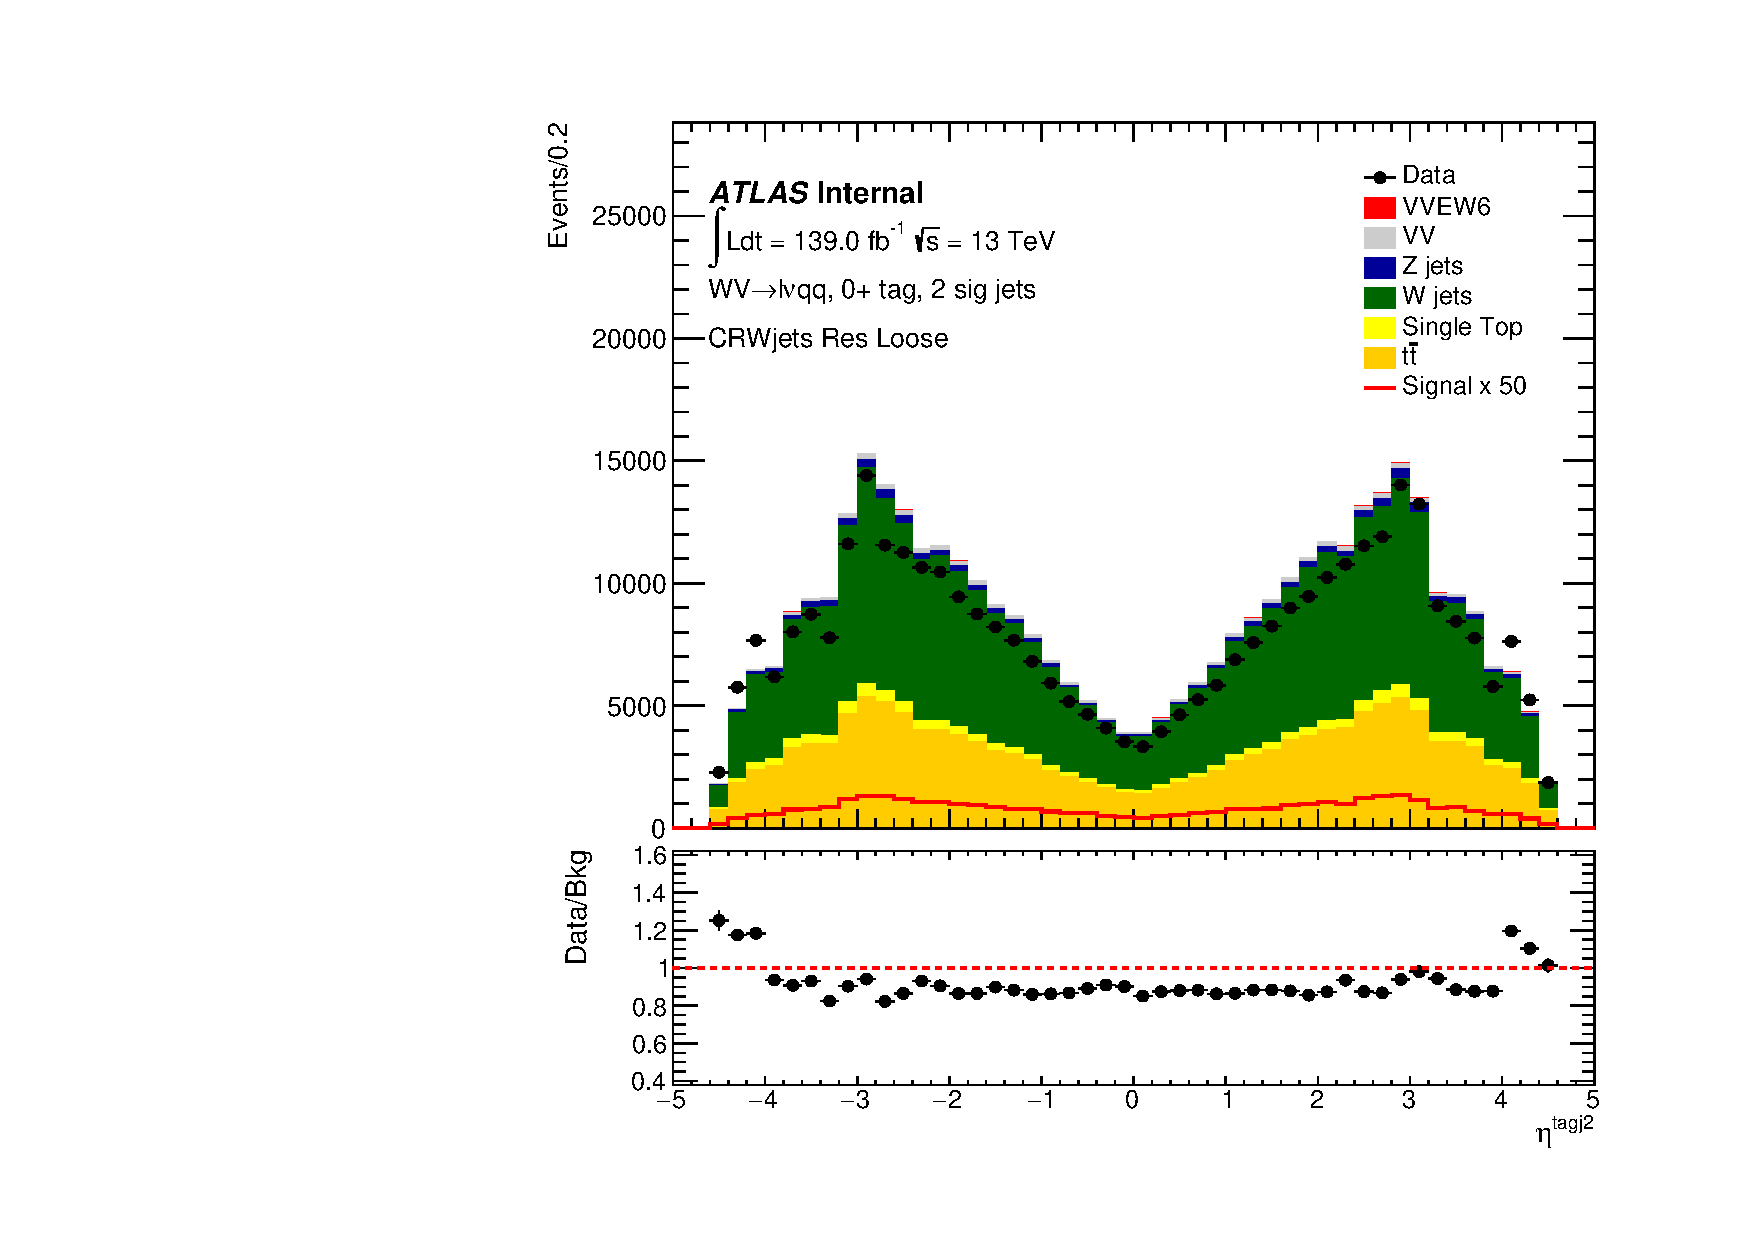
\includegraphics[width=0.3\textwidth]{figures/CRPlots/CRWjets_Res_Loose/stacked_plot_resolved_tagJ2_eta.pdf}} \\
    \subfloat[]{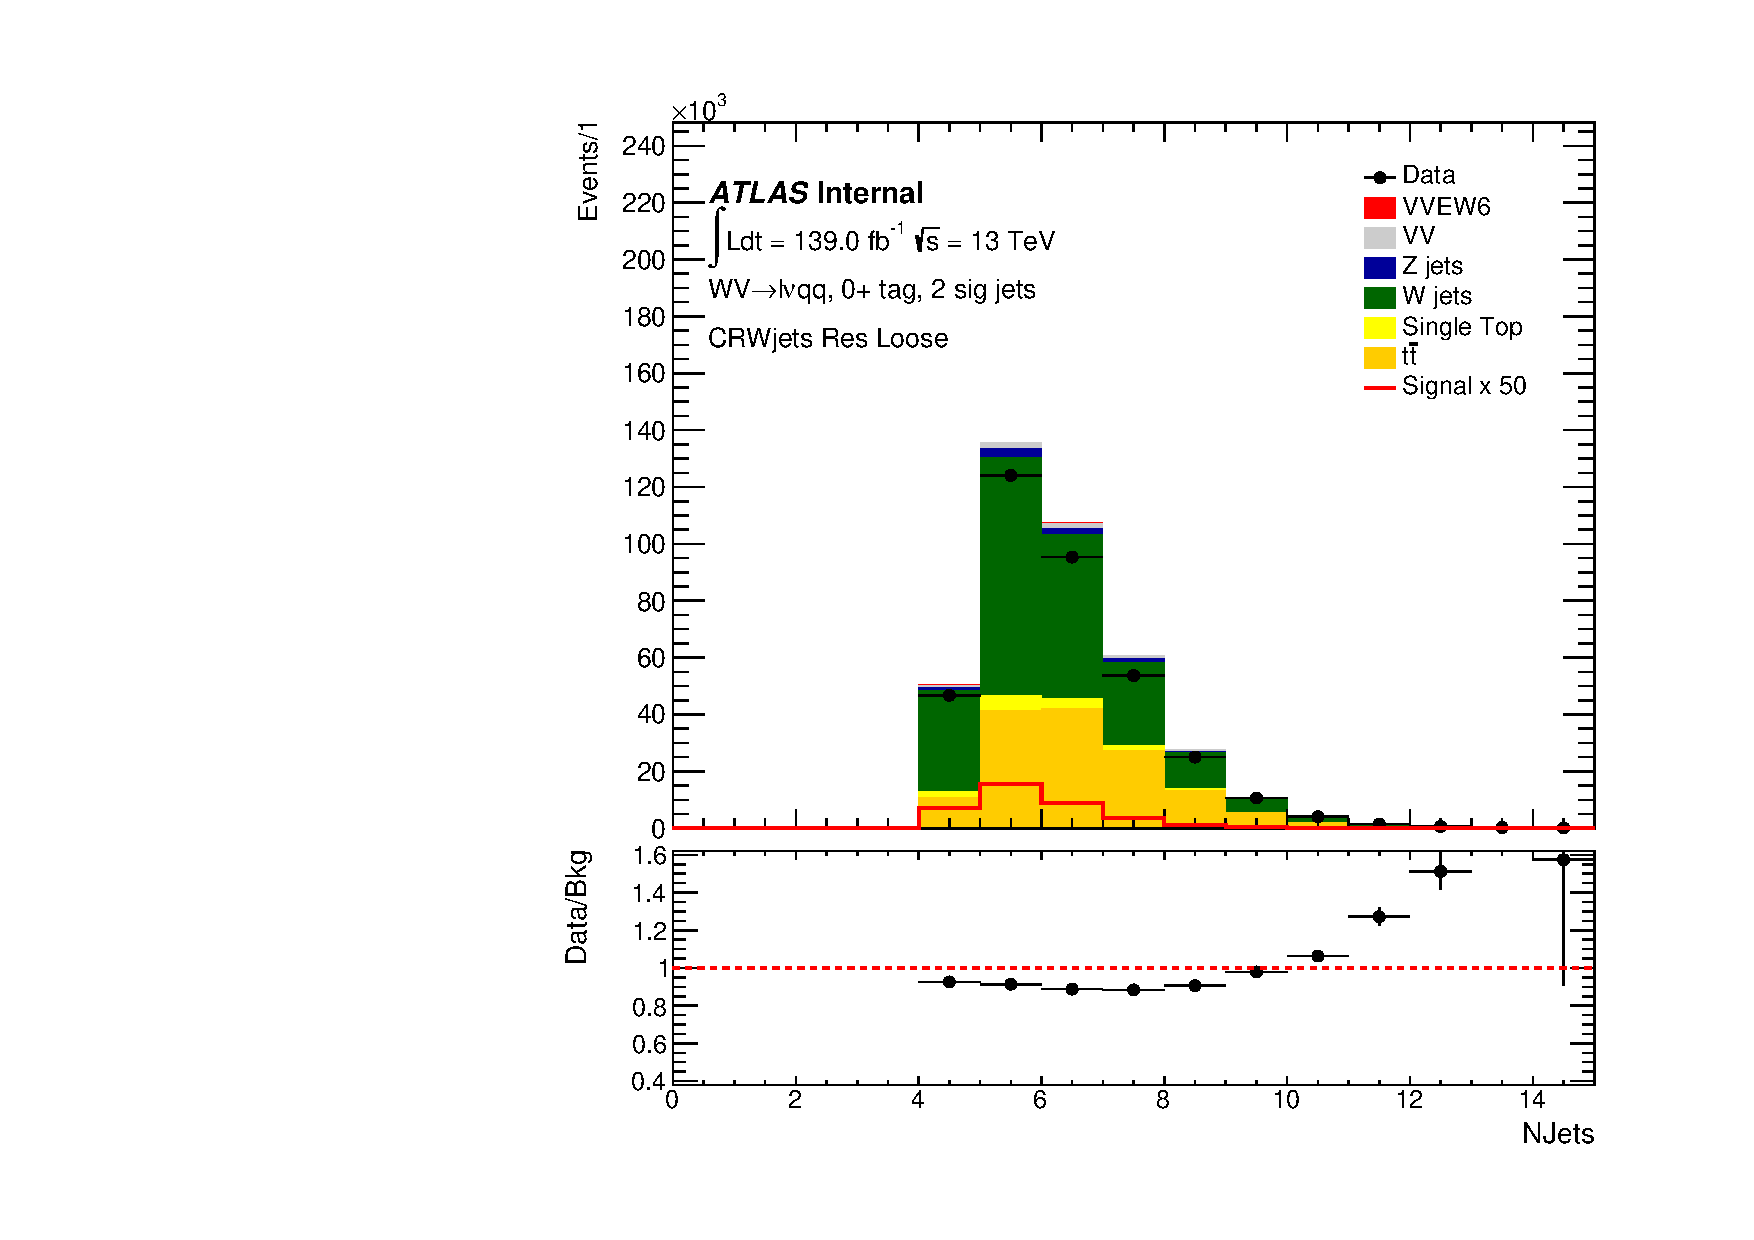
\includegraphics[width=0.3\textwidth]{figures/CRPlots/CRWjets_Res_Loose/stacked_plot_NJets.pdf}}
    \subfloat[]{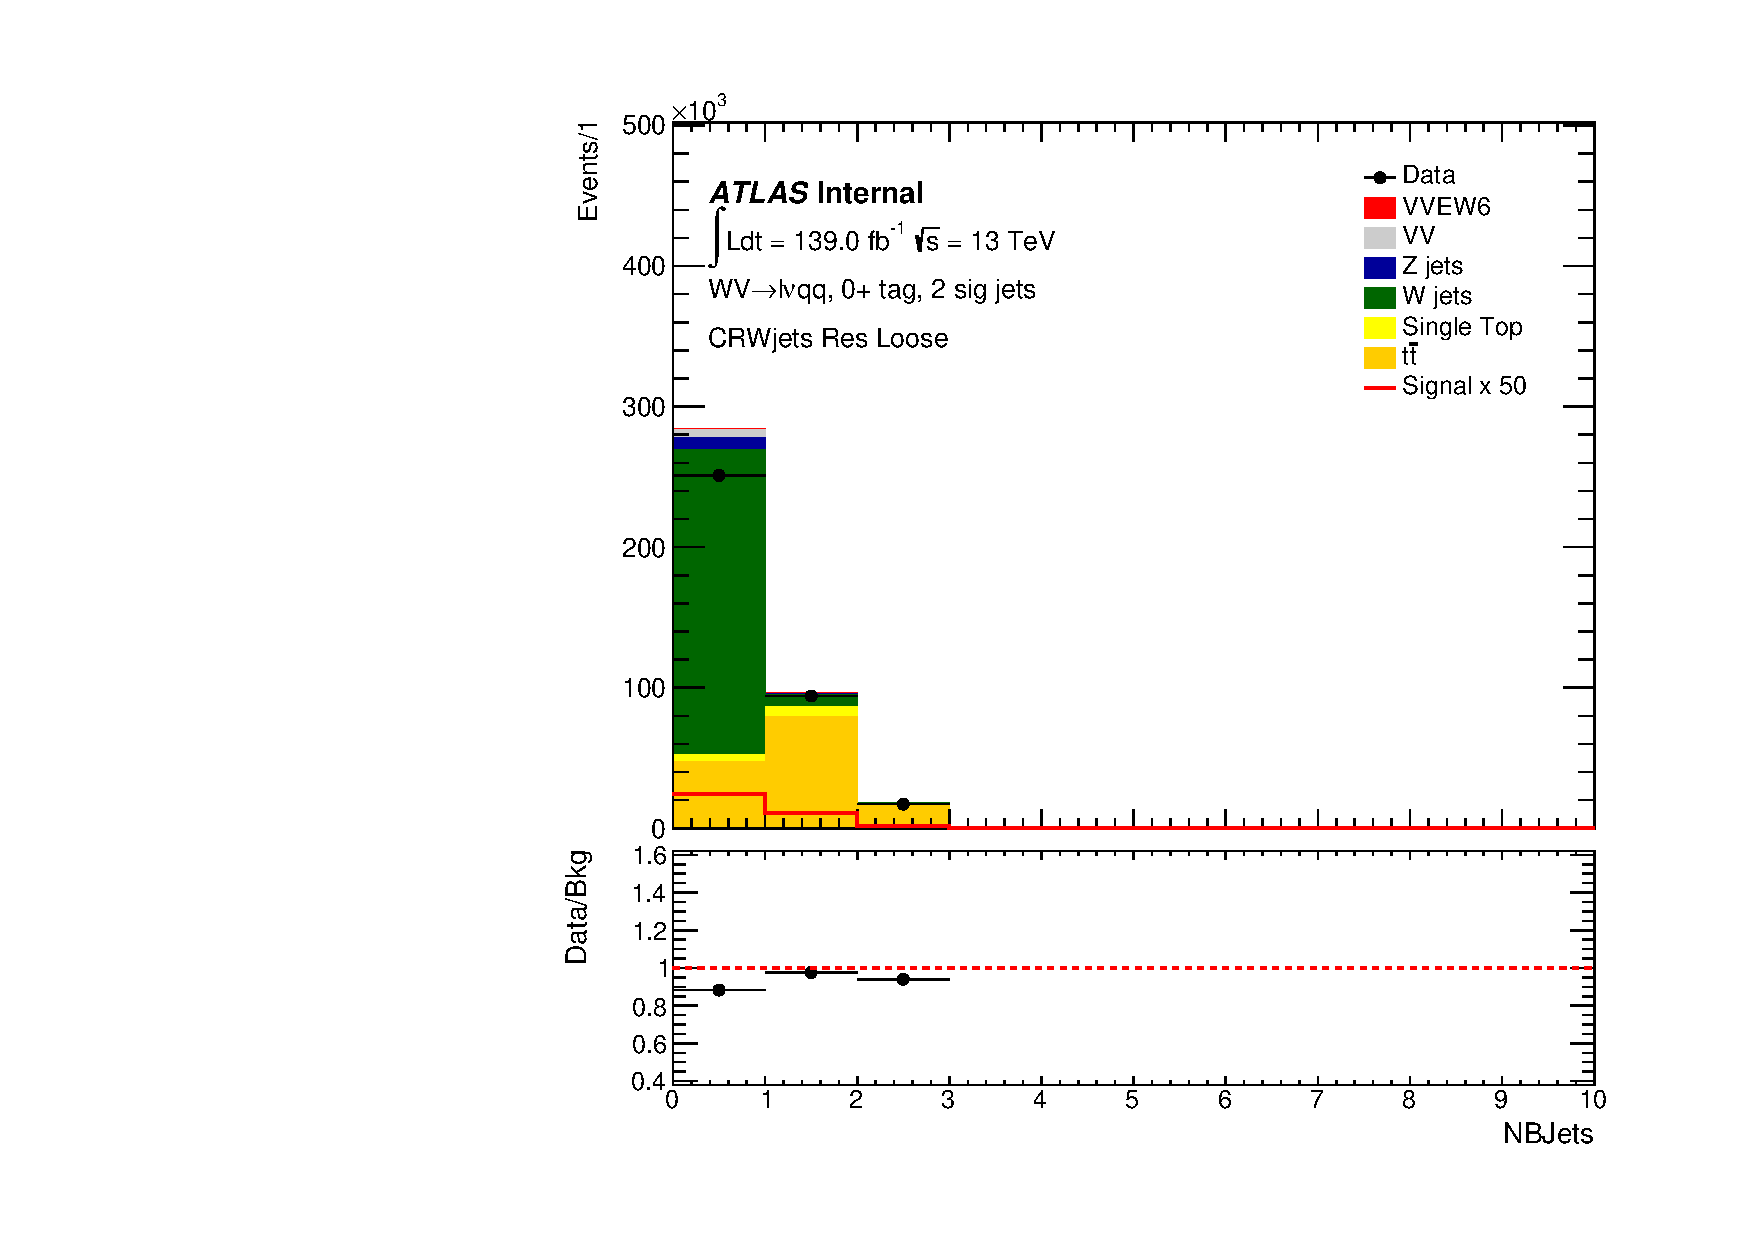
\includegraphics[width=0.3\textwidth]{figures/CRPlots/CRWjets_Res_Loose/stacked_plot_NBJets.pdf}}
    \subfloat[]{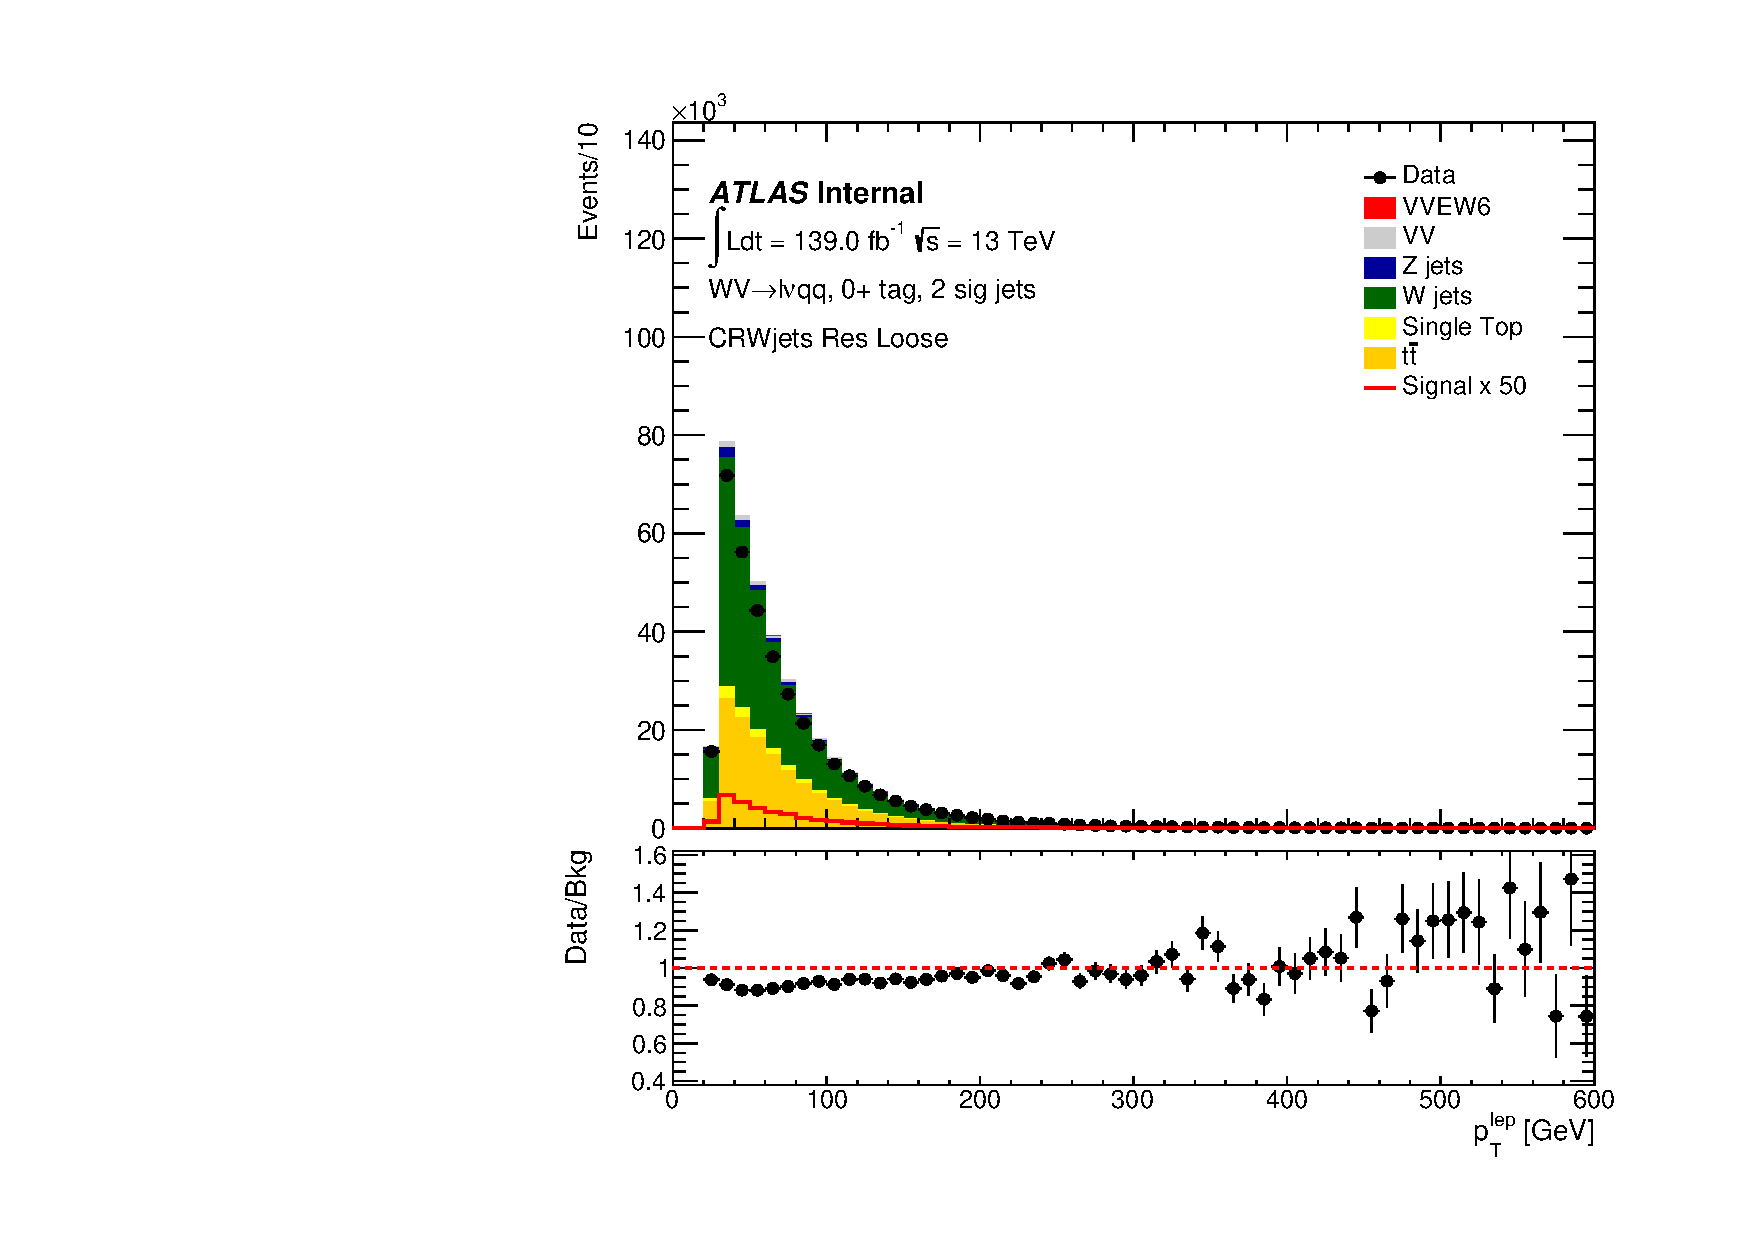
\includegraphics[width=0.3\textwidth]{figures/CRPlots/CRWjets_Res_Loose/stacked_plot_lep_pt.pdf}}  %%\\
    \caption{Data-MC checks for the resolved loose \Wjets control region in the \olep channel.}
    \label{fig:CRWjetResLoosePlots1Lep}
\end{figure}


\begin{figure}[ht]
    \centering
    \subfloat[]{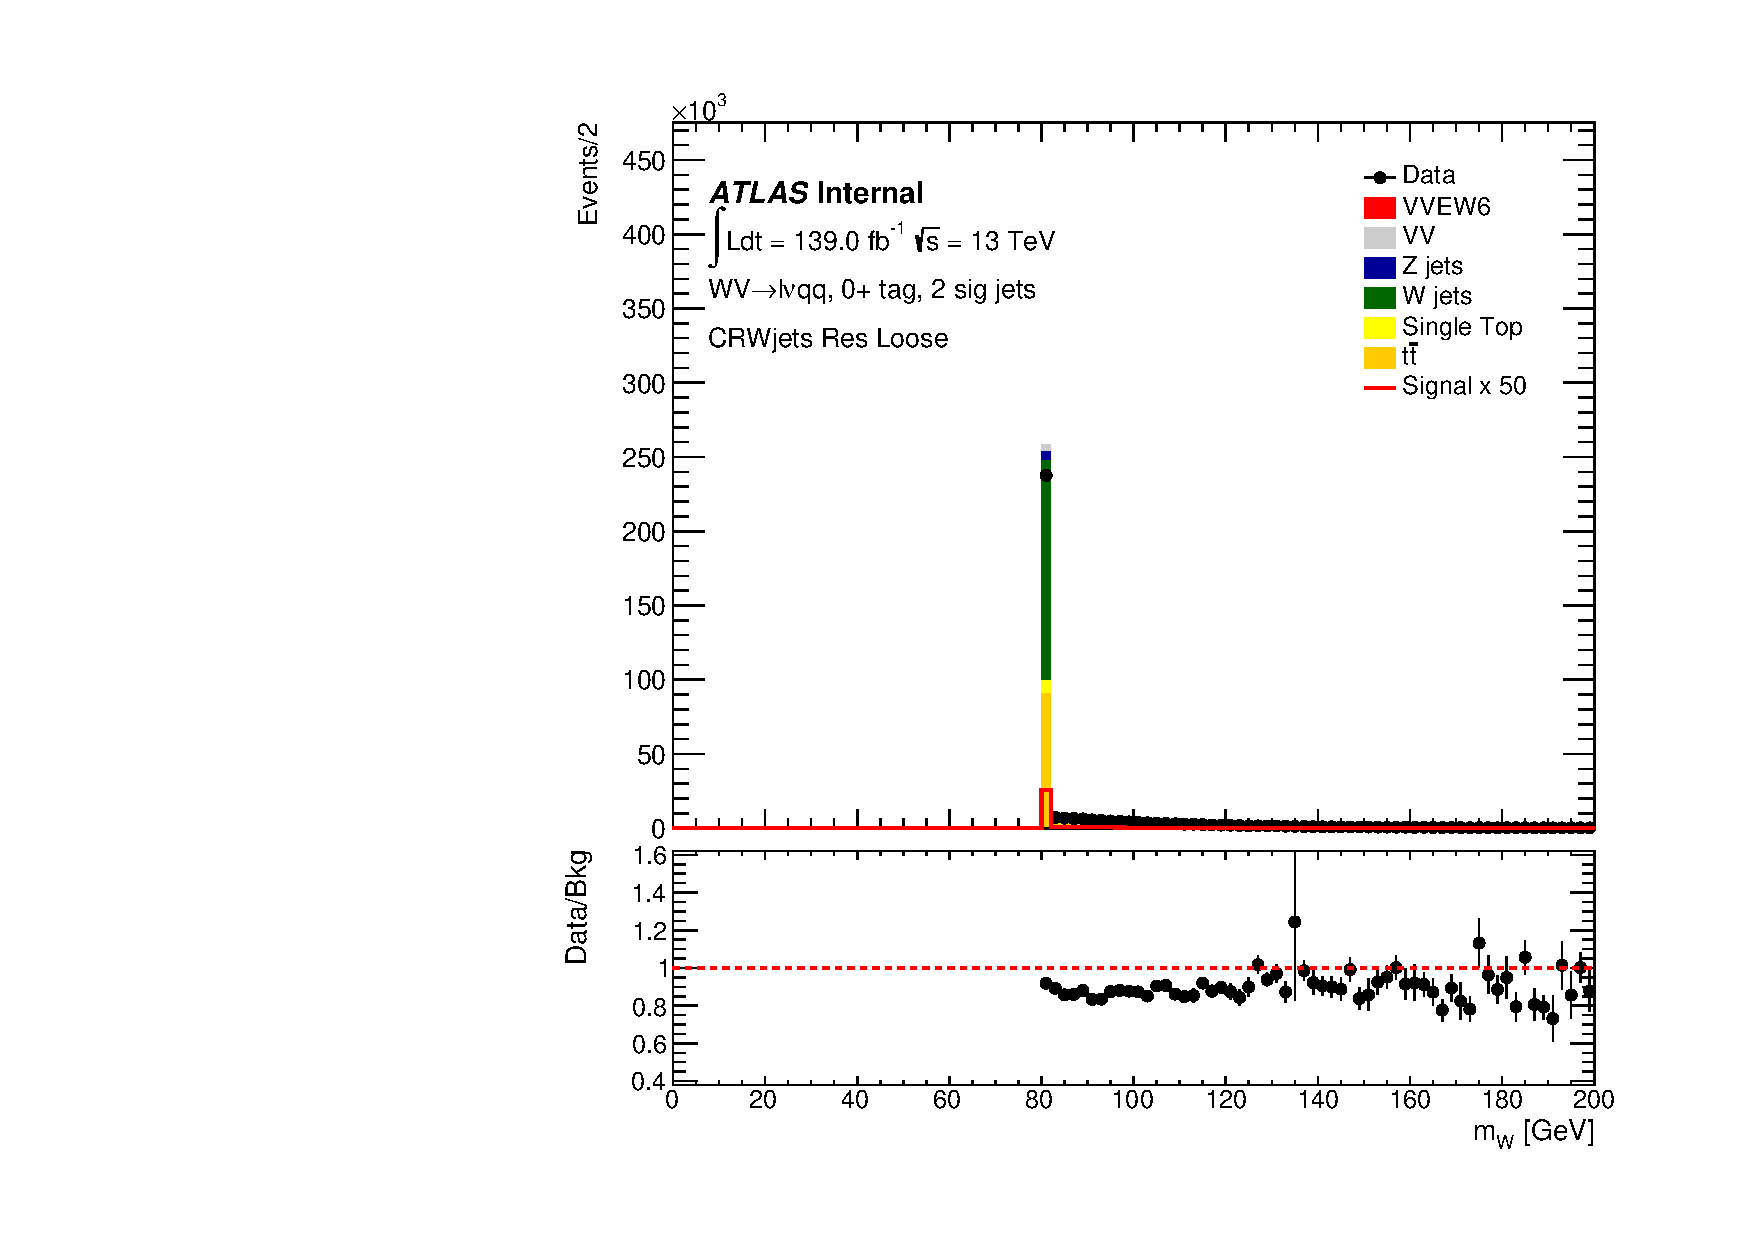
\includegraphics[width=0.3\textwidth]{figures/CRPlots/CRWjets_Res_Loose/stacked_plot_W_m.pdf}}
    \subfloat[]{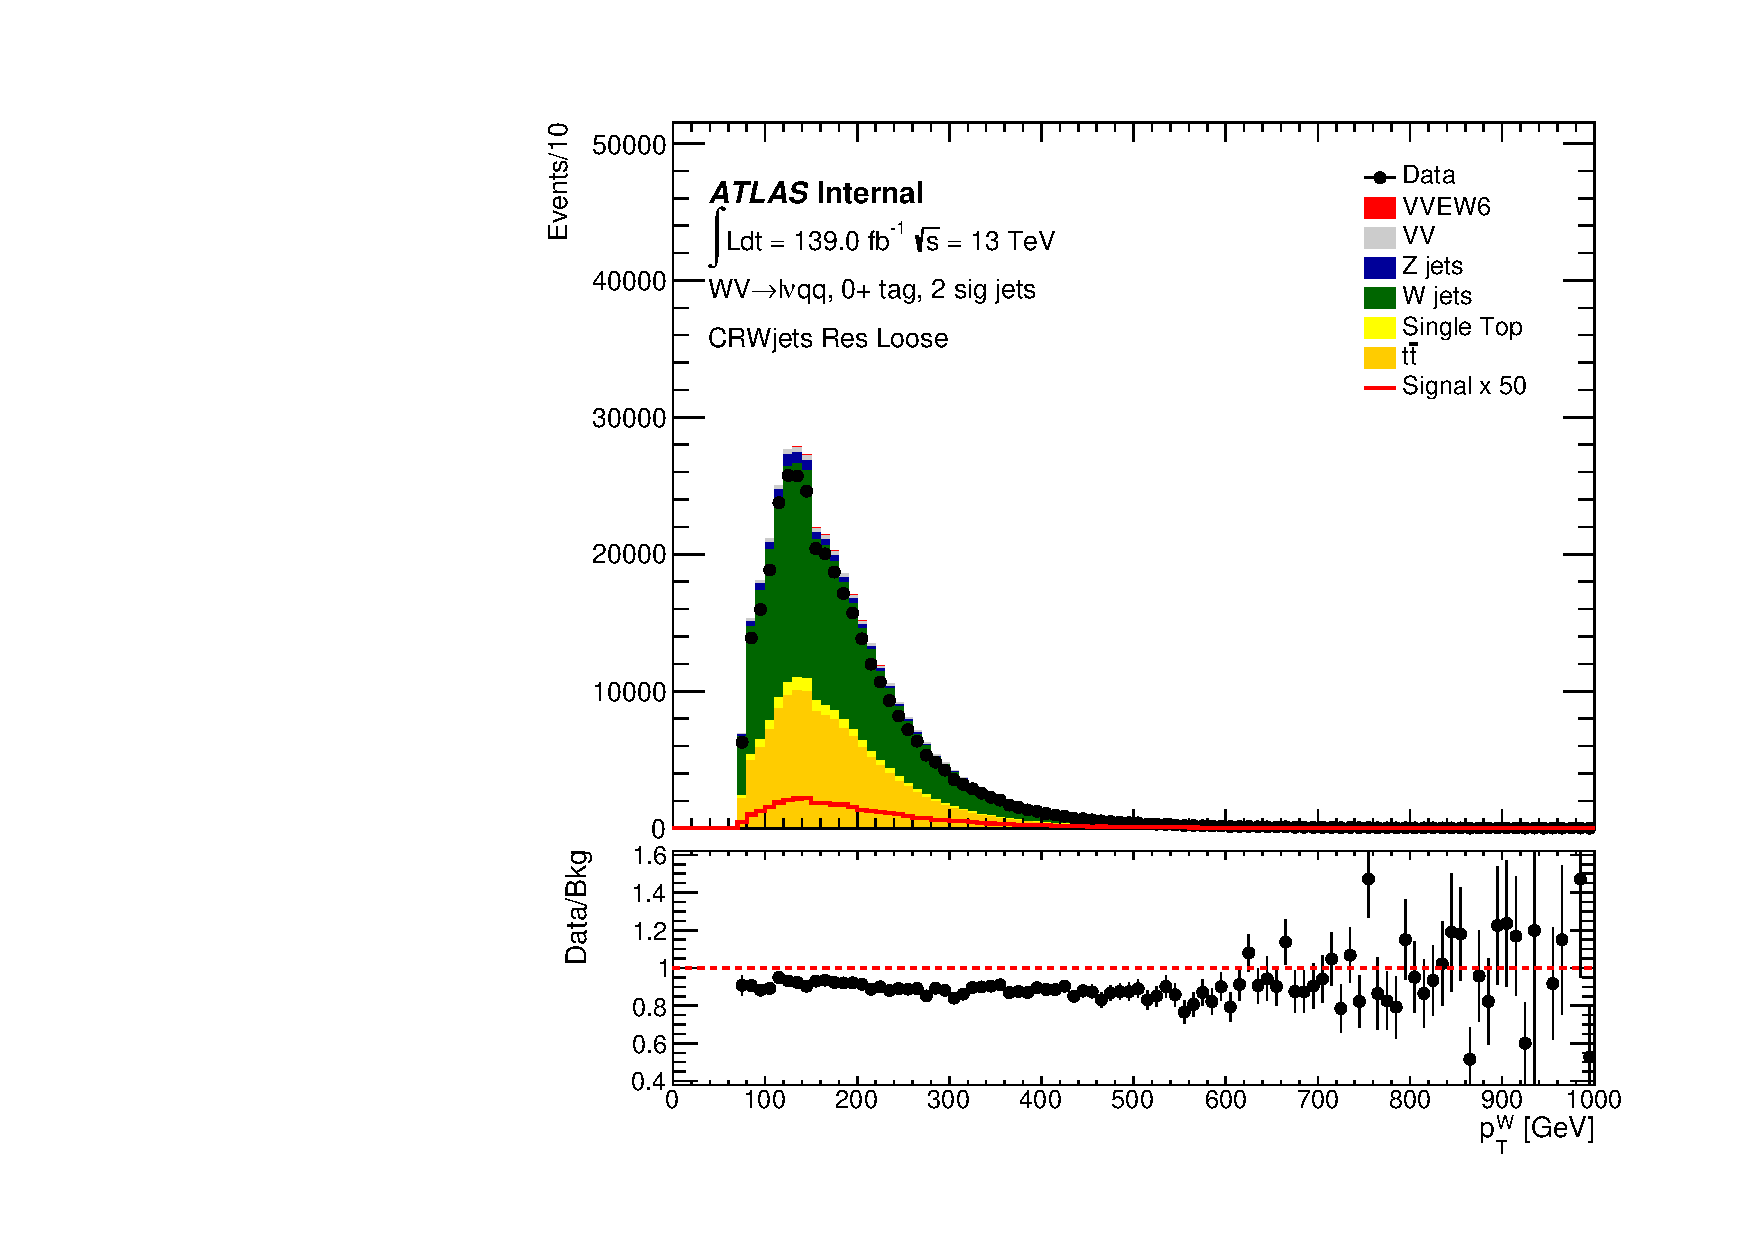
\includegraphics[width=0.3\textwidth]{figures/CRPlots/CRWjets_Res_Loose/stacked_plot_W_pt.pdf}}
    \subfloat[]{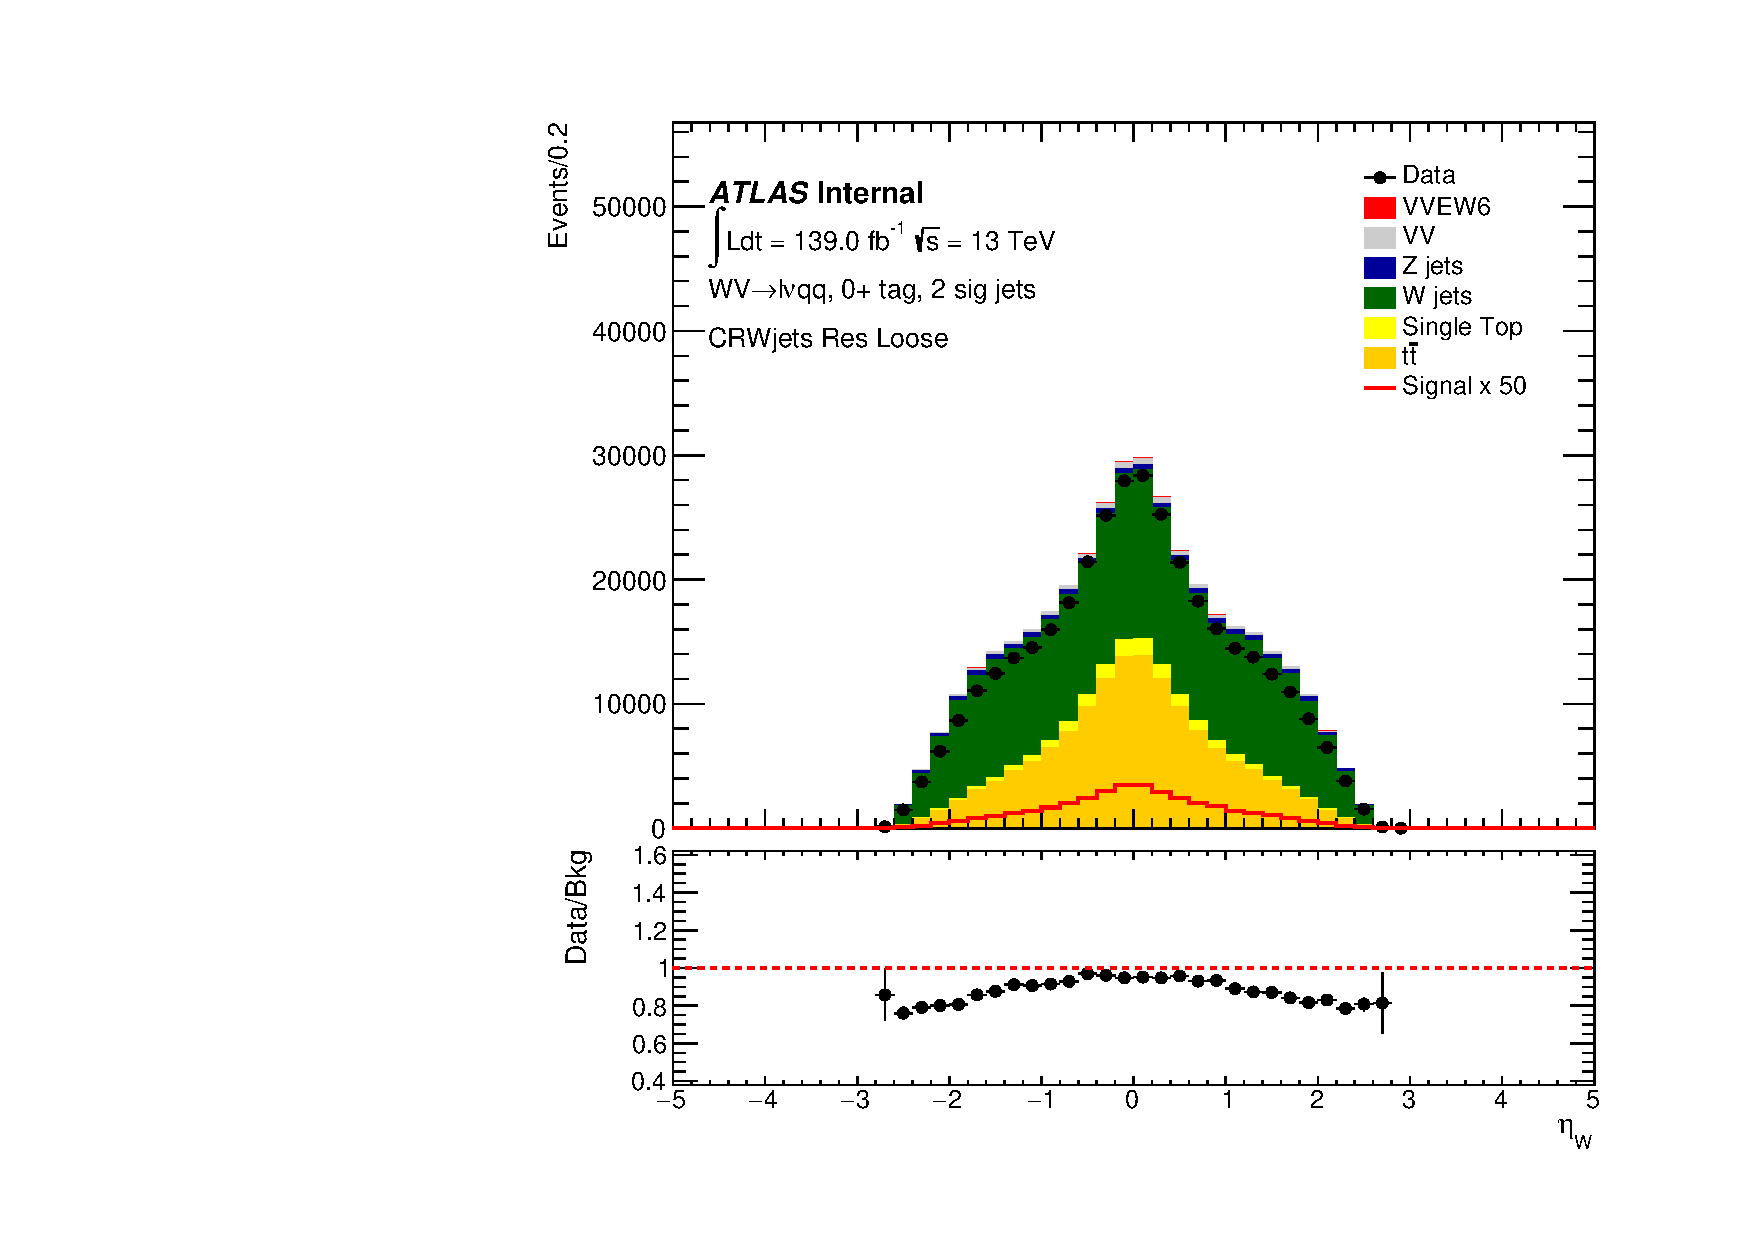
\includegraphics[width=0.3\textwidth]{figures/CRPlots/CRWjets_Res_Loose/stacked_plot_W_eta.pdf}} \\
    \subfloat[]{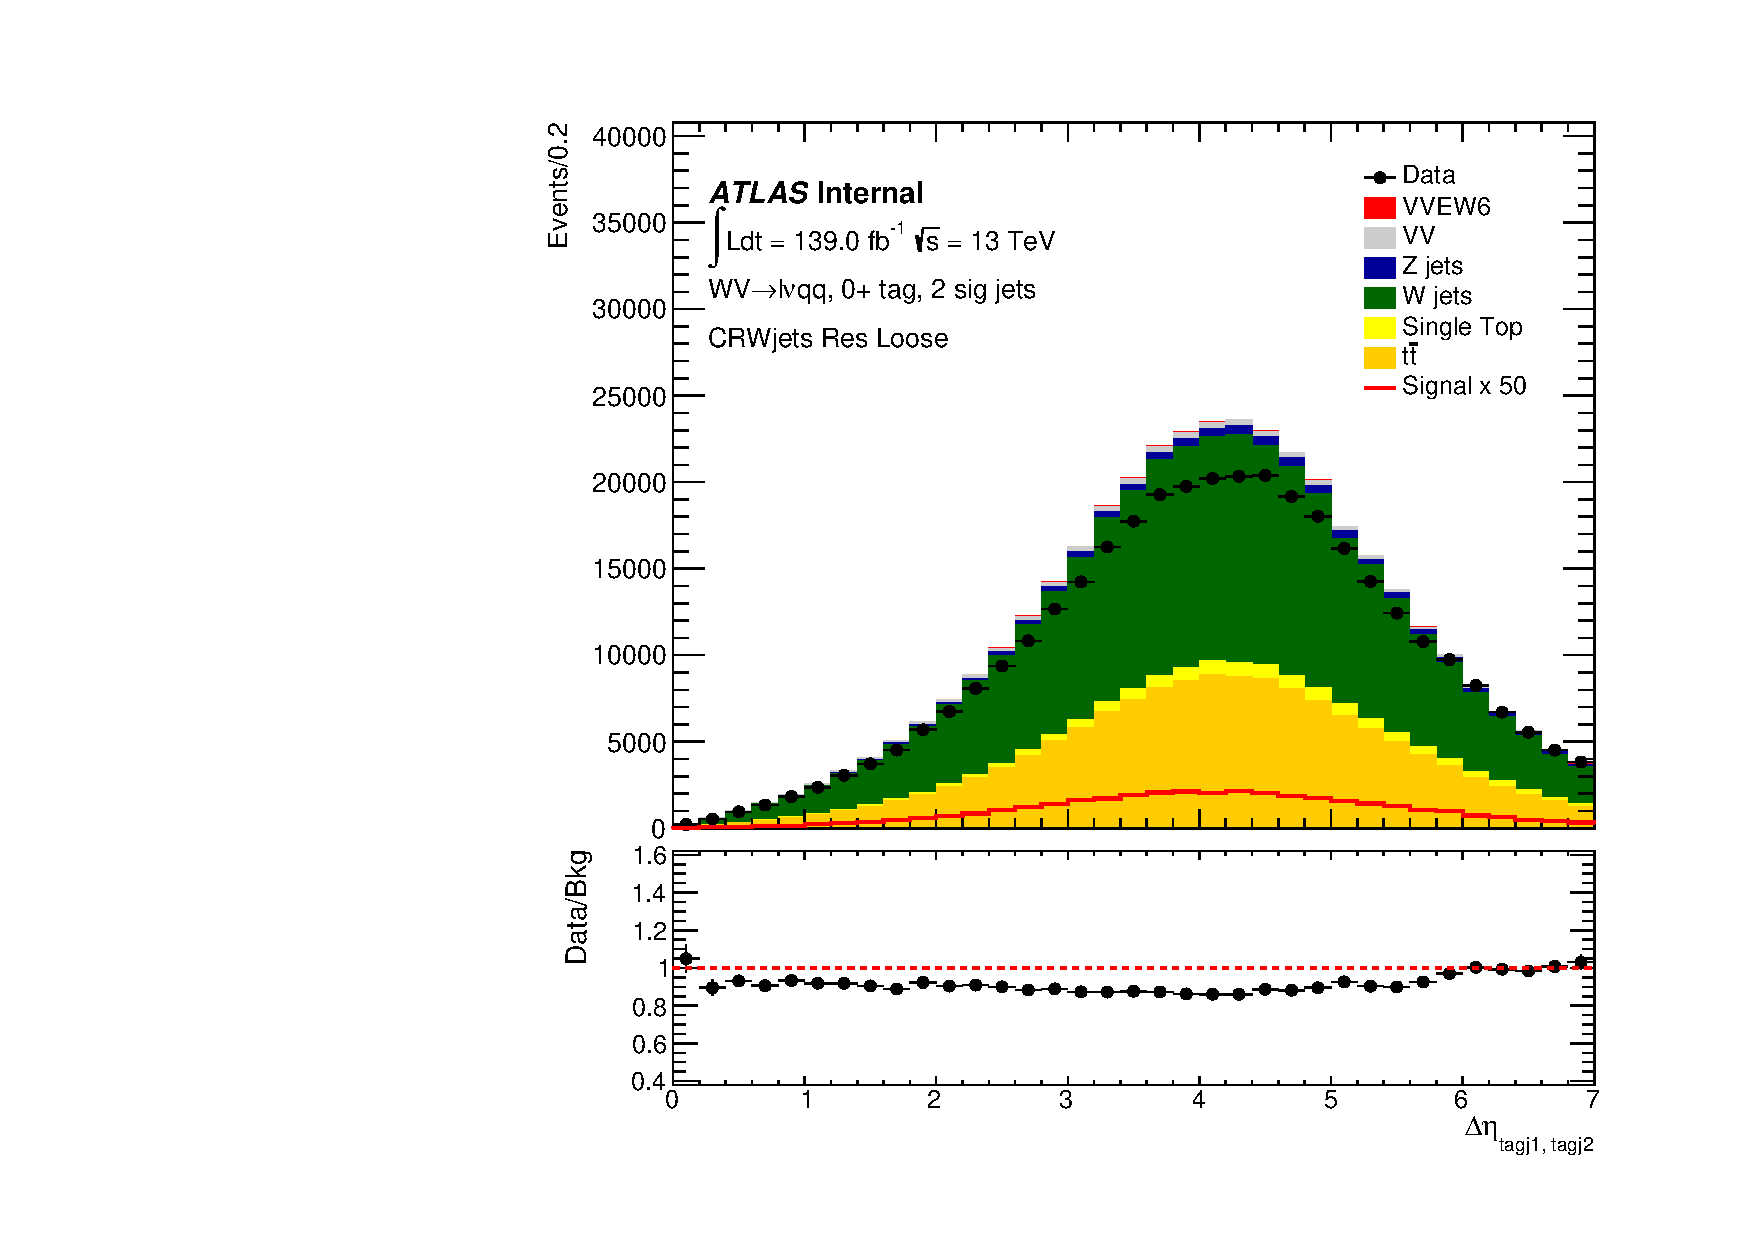
\includegraphics[width=0.3\textwidth]{figures/CRPlots/CRWjets_Res_Loose/stacked_plot_resolved_tagJdEta.pdf}}
    \subfloat[]{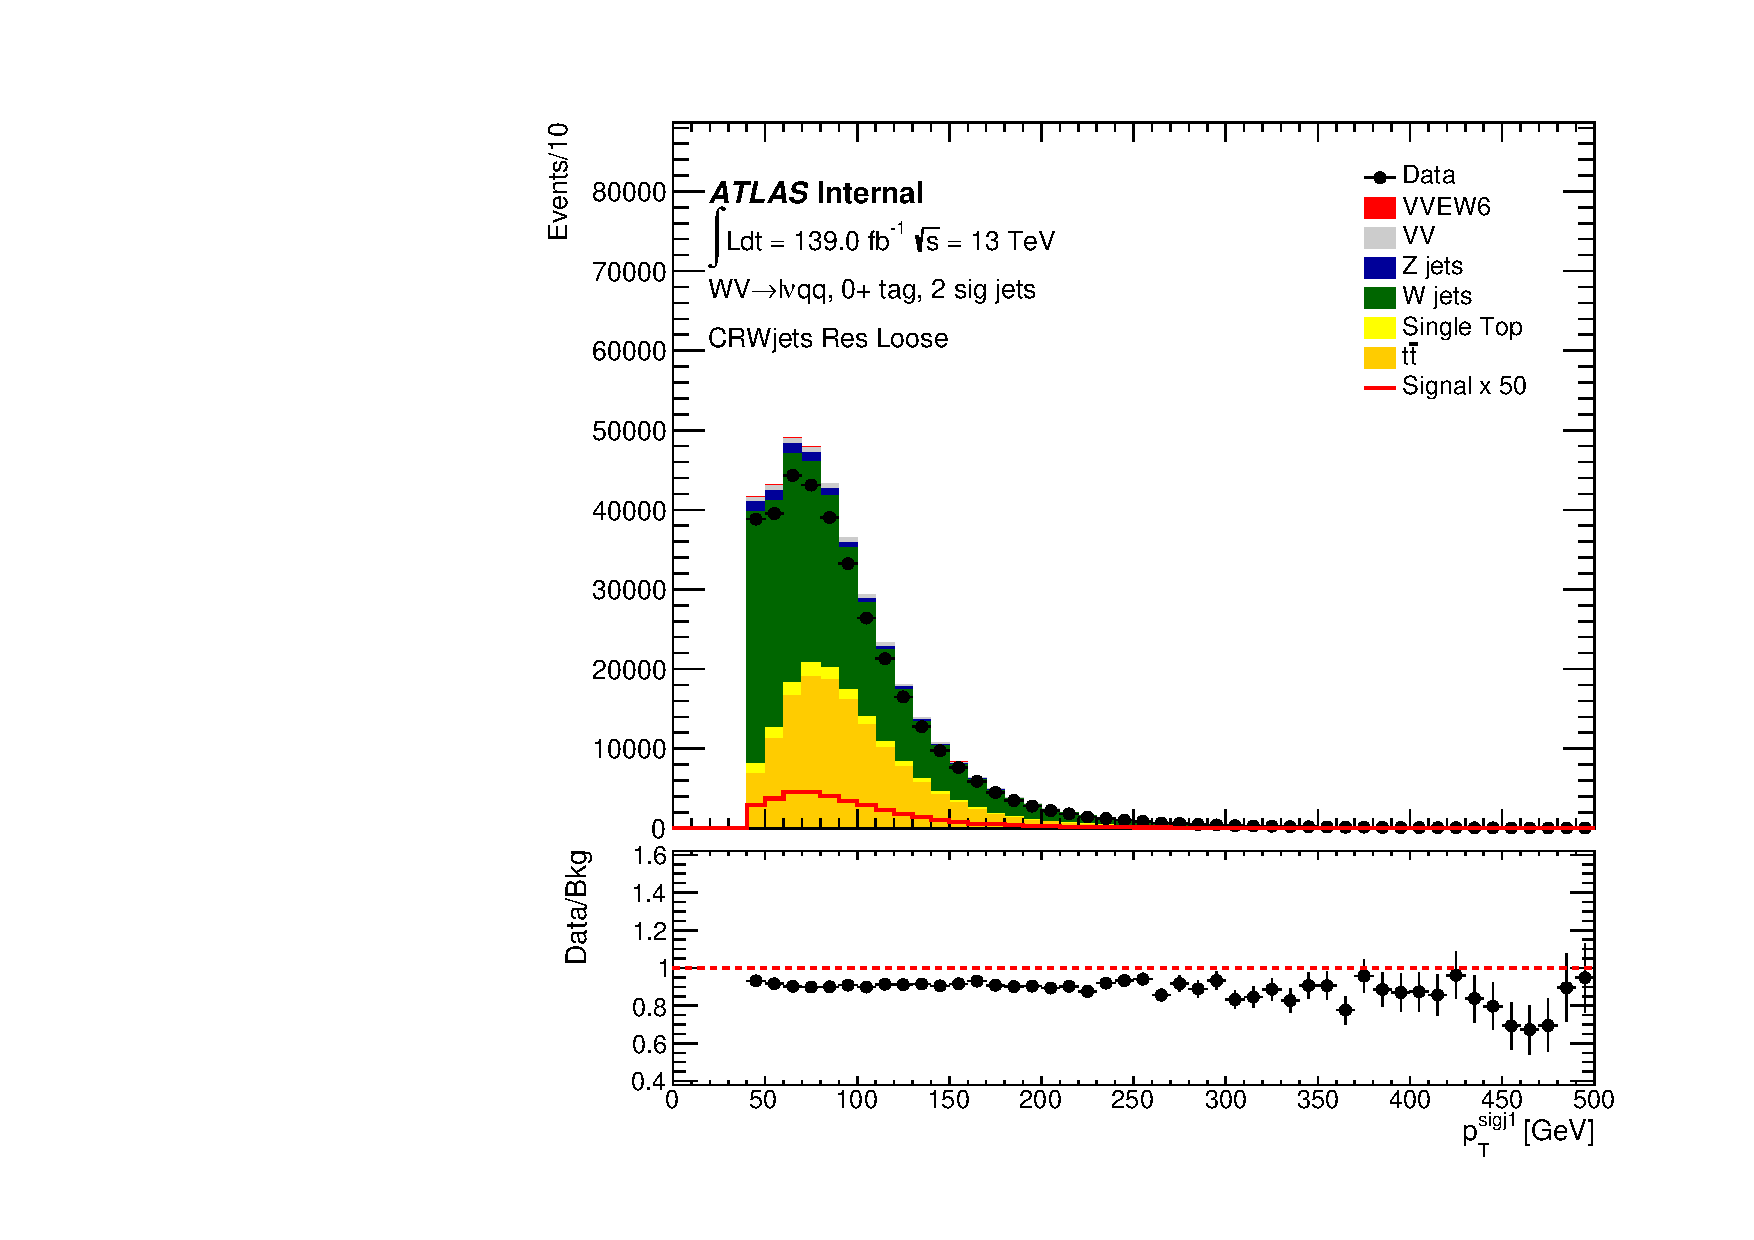
\includegraphics[width=0.3\textwidth]{figures/CRPlots/CRWjets_Res_Loose/stacked_plot_sigJ1_pt.pdf}}
    \subfloat[]{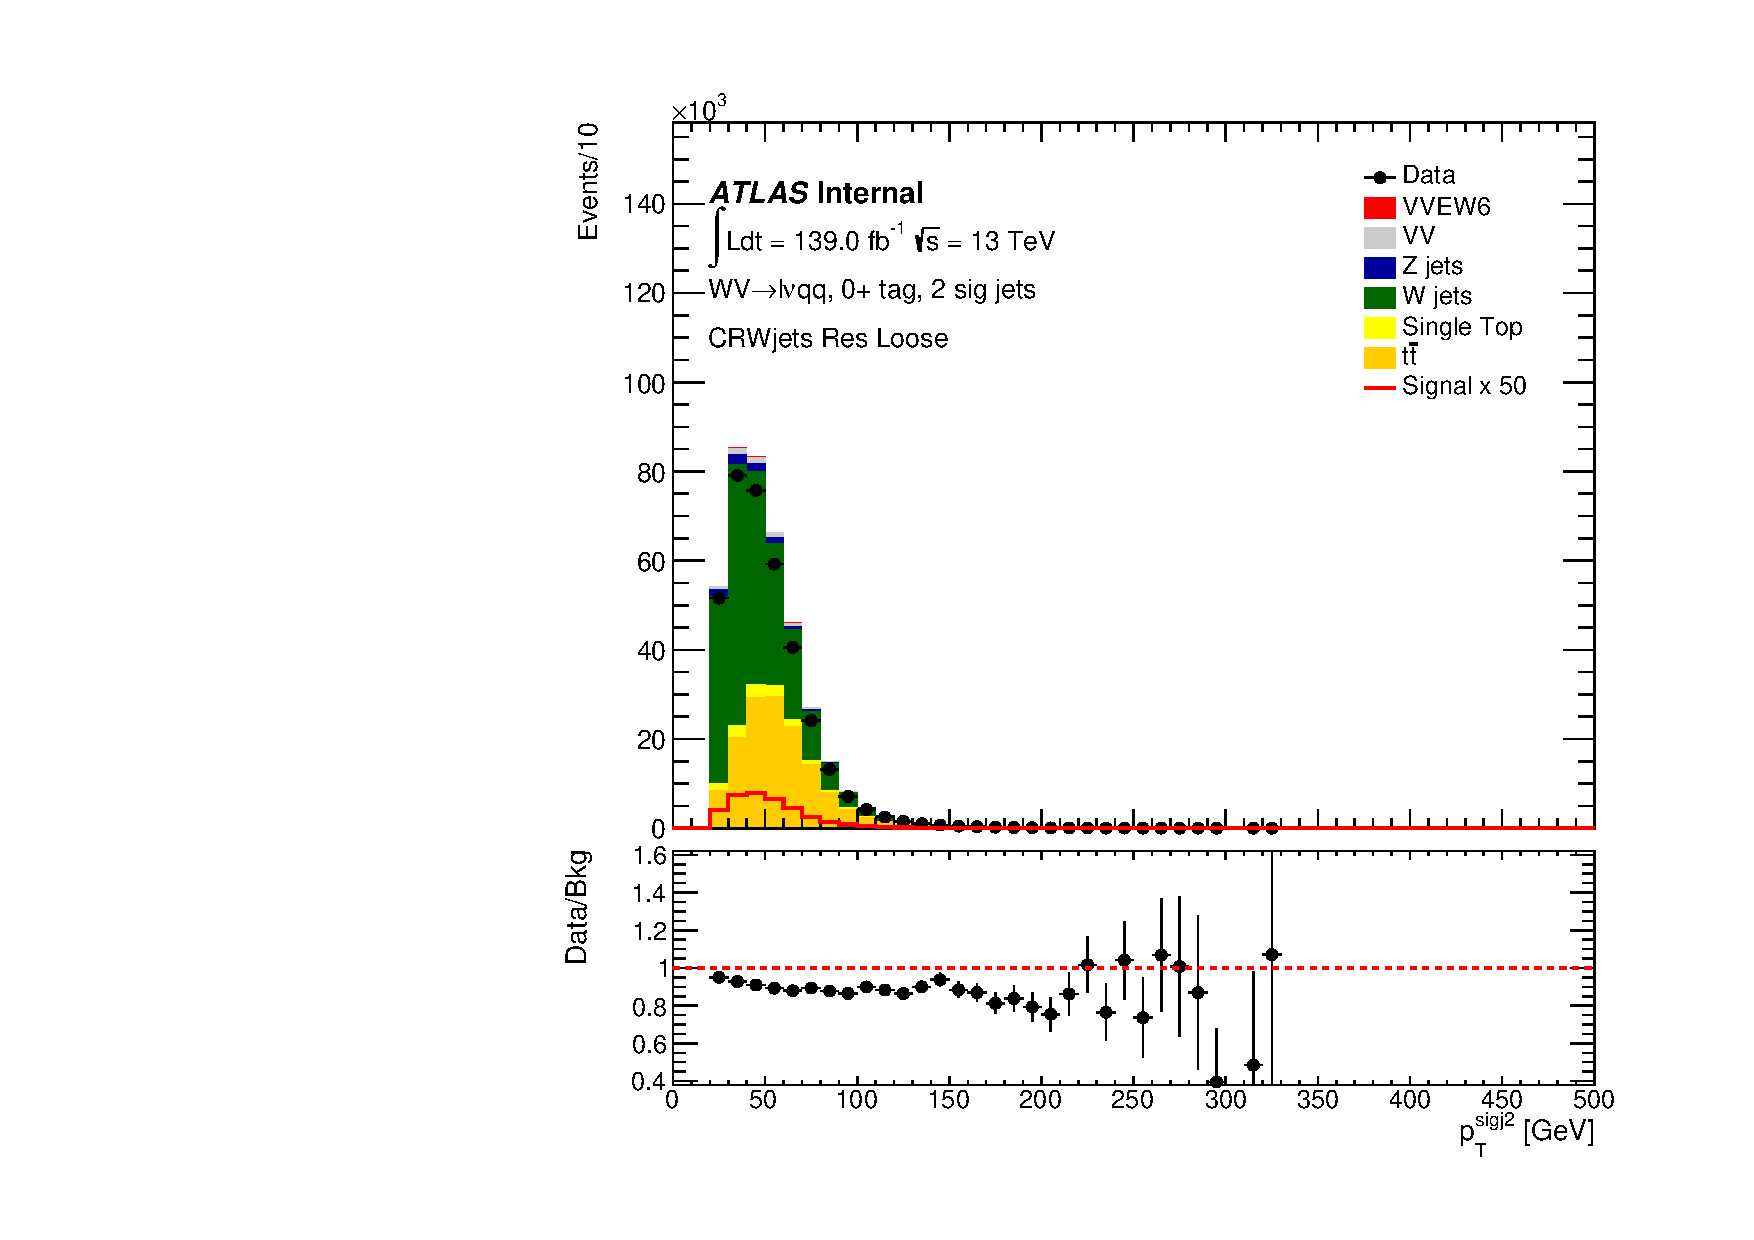
\includegraphics[width=0.3\textwidth]{figures/CRPlots/CRWjets_Res_Loose/stacked_plot_sigJ2_pt.pdf}} \\
    \subfloat[]{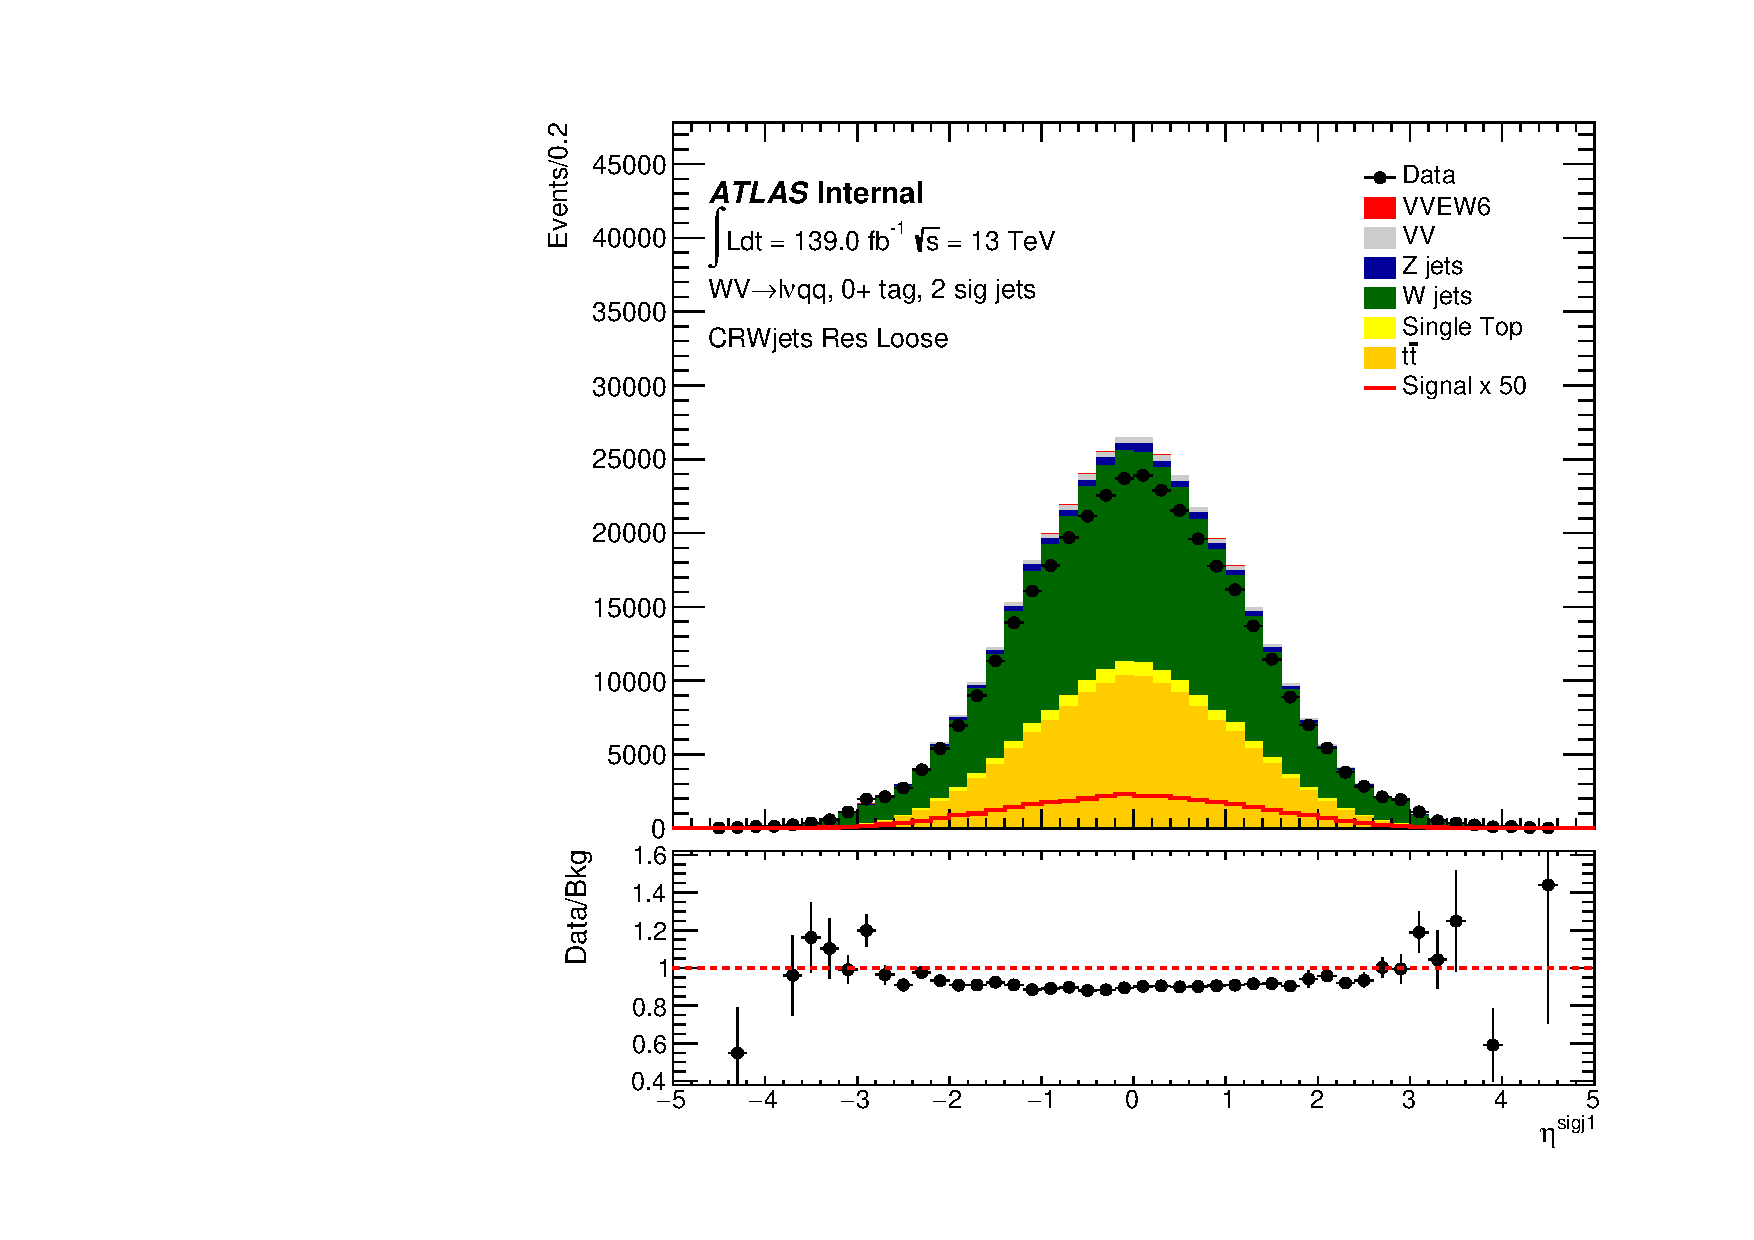
\includegraphics[width=0.3\textwidth]{figures/CRPlots/CRWjets_Res_Loose/stacked_plot_sigJ1_eta.pdf}}
    \subfloat[]{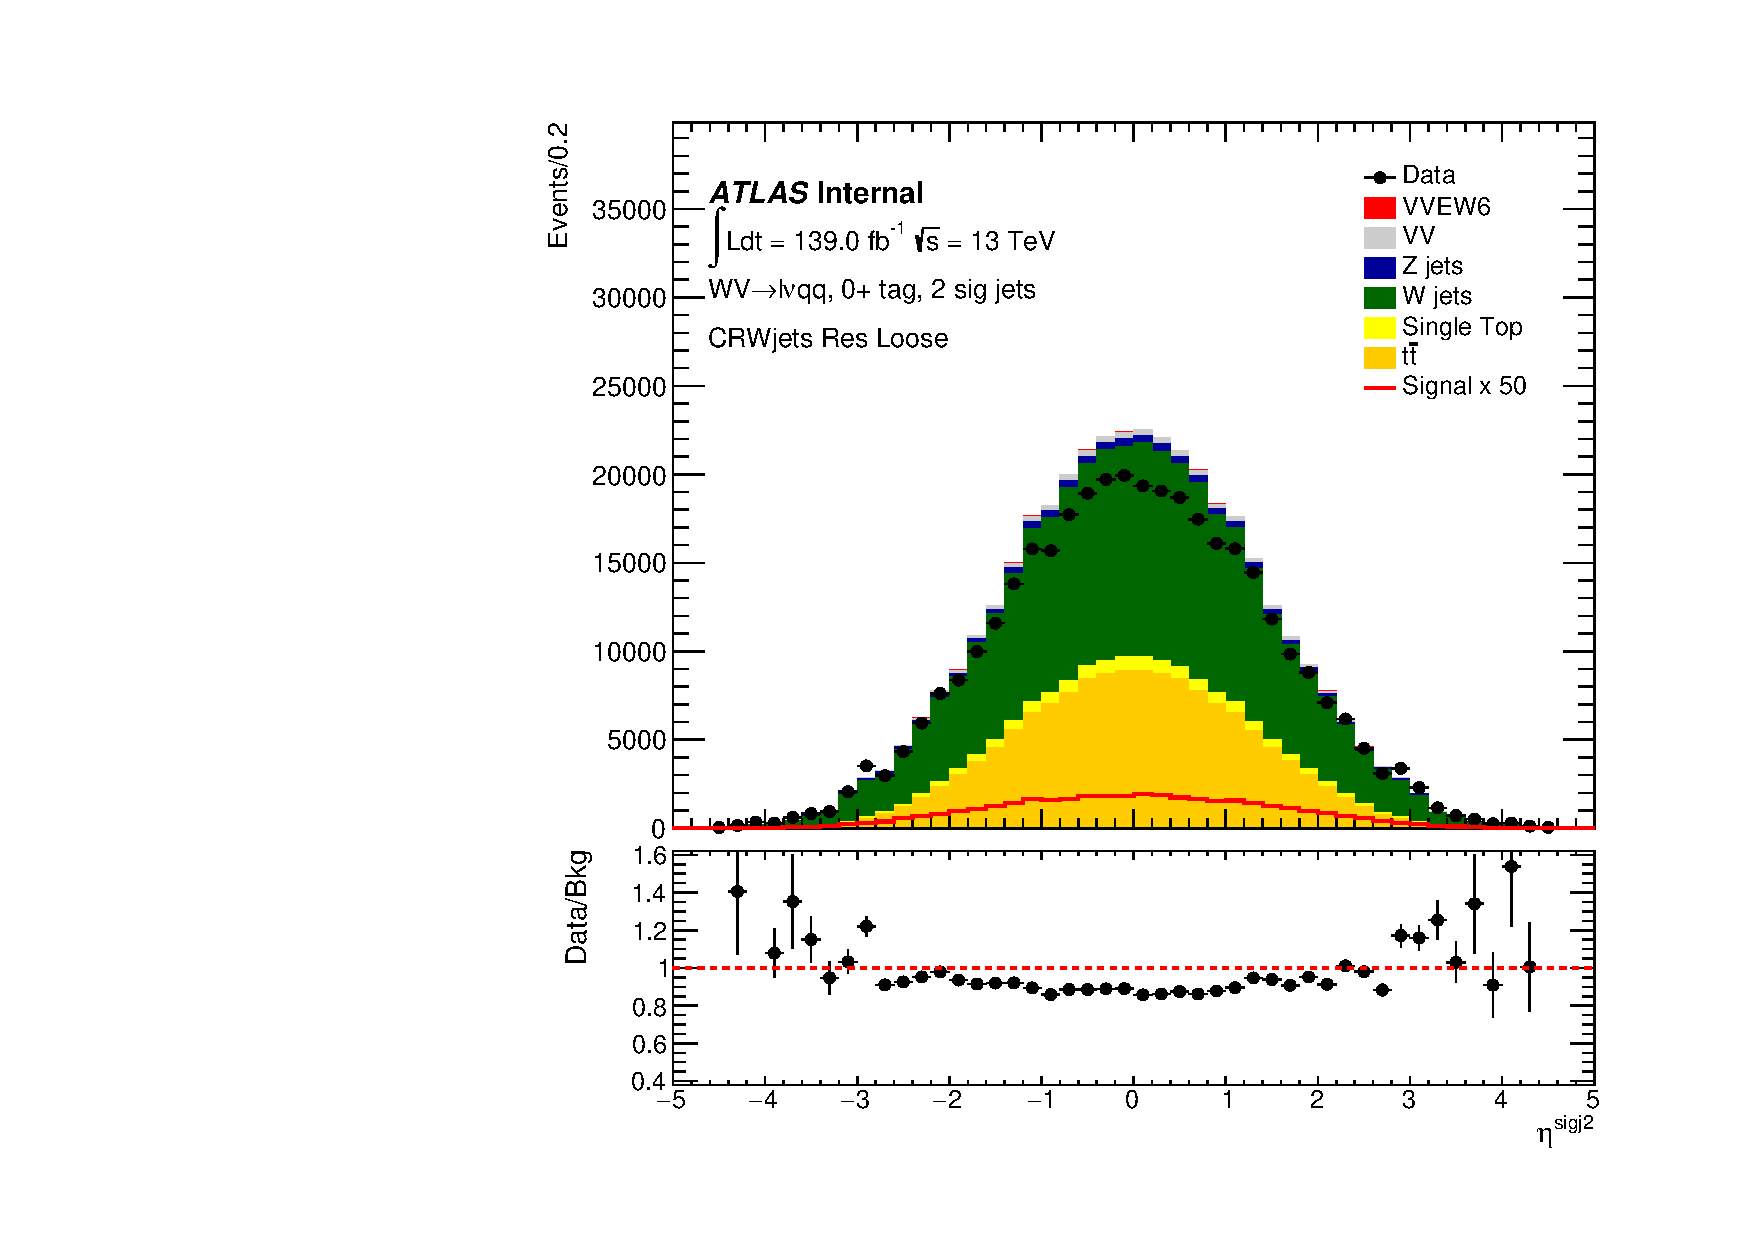
\includegraphics[width=0.3\textwidth]{figures/CRPlots/CRWjets_Res_Loose/stacked_plot_sigJ2_eta.pdf}} \\
    \subfloat[]{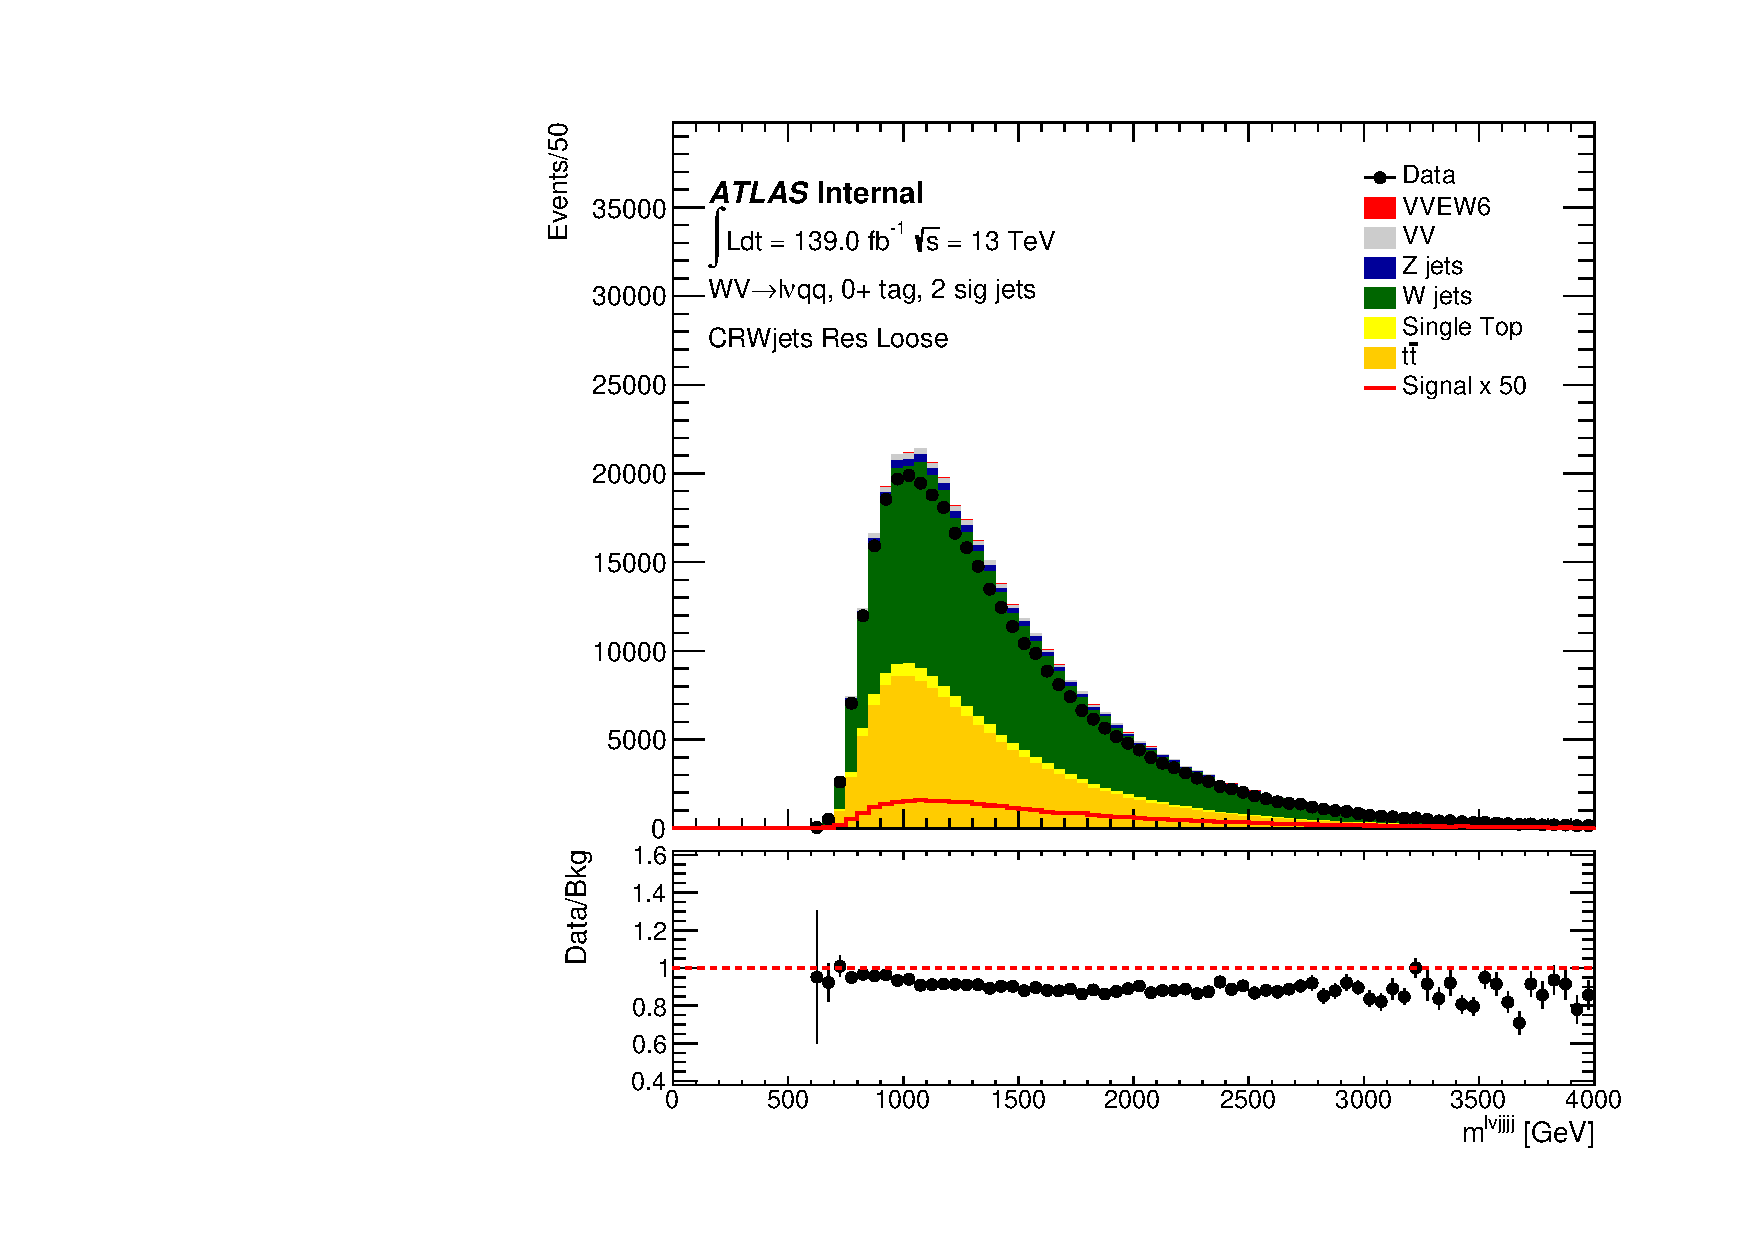
\includegraphics[width=0.3\textwidth]{figures/CRPlots/CRWjets_Res_Loose/stacked_plot_lvjjjjmass.pdf}}
    \subfloat[]{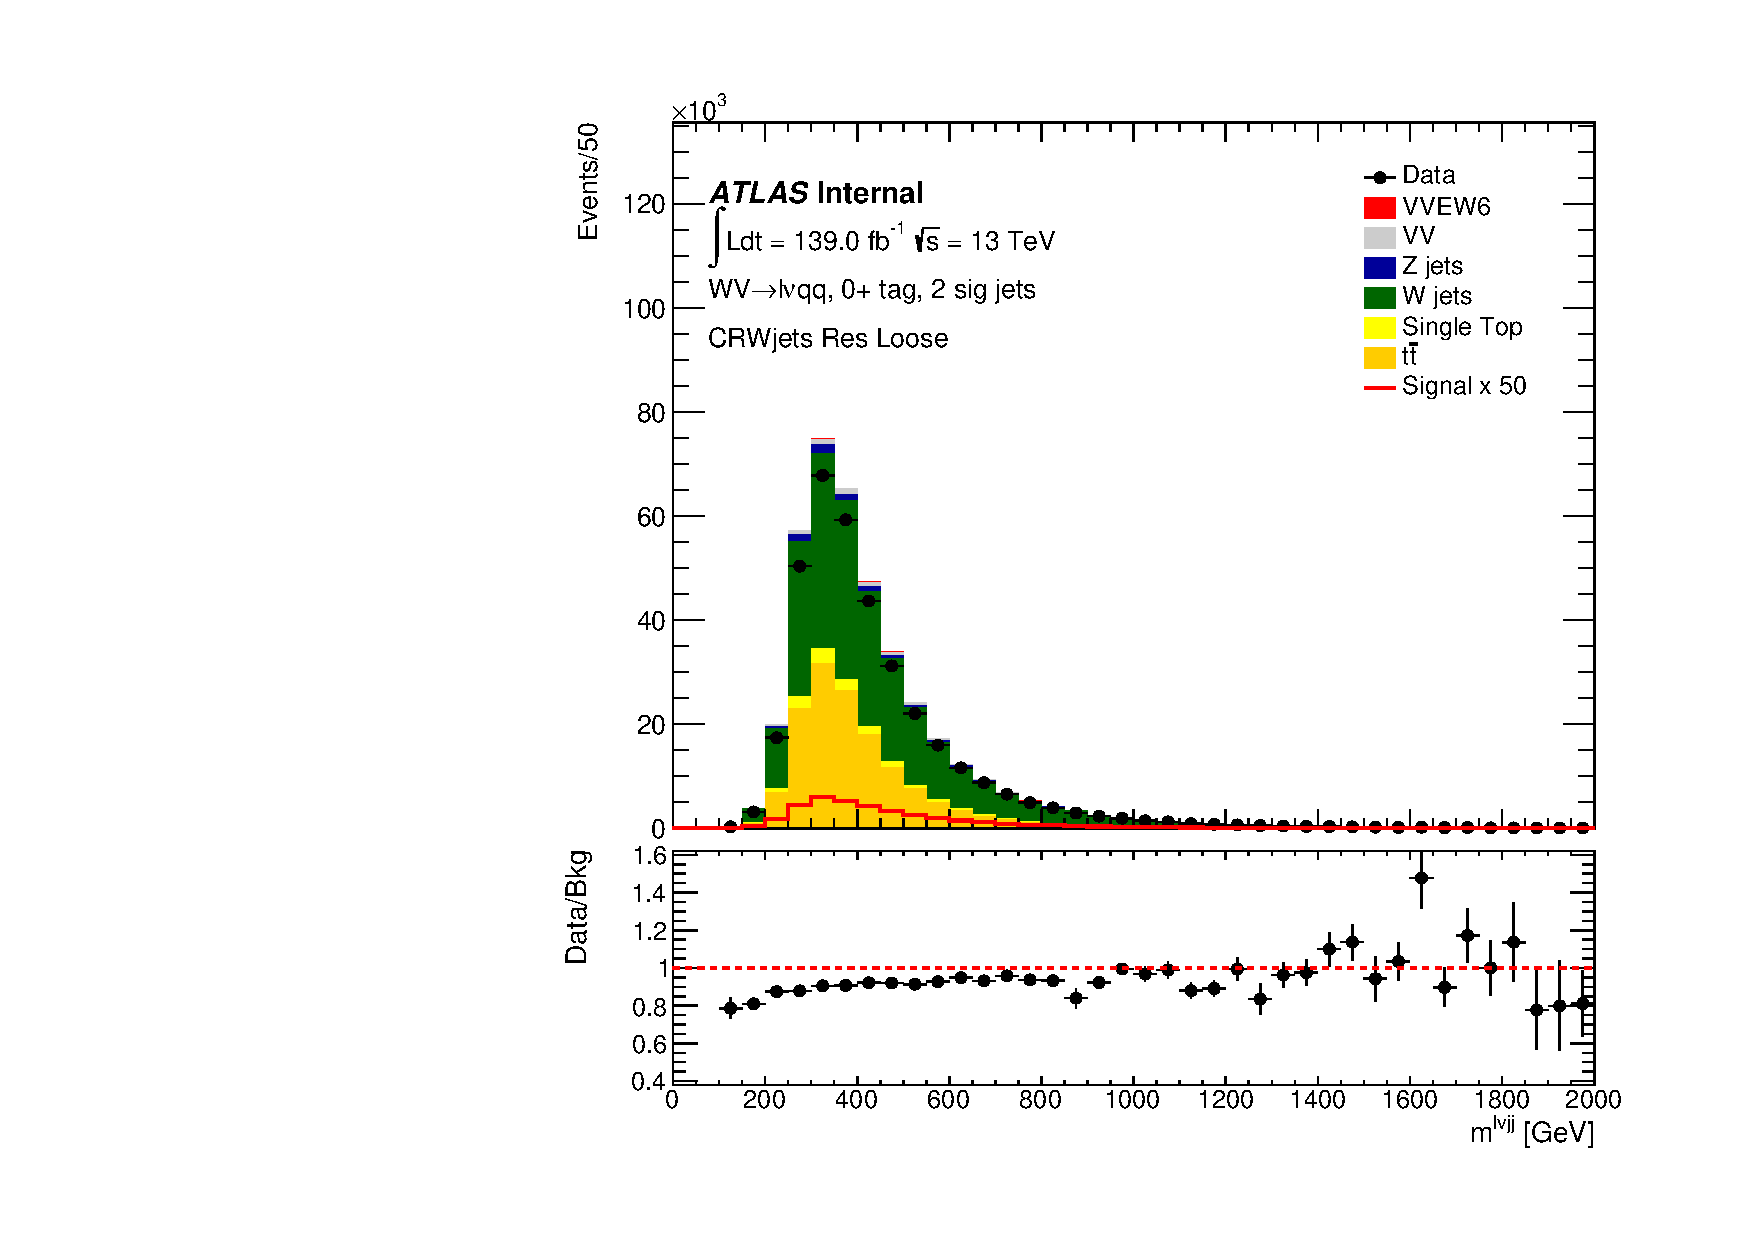
\includegraphics[width=0.3\textwidth]{figures/CRPlots/CRWjets_Res_Loose/stacked_plot_lvjjmass.pdf}}
    \subfloat[]{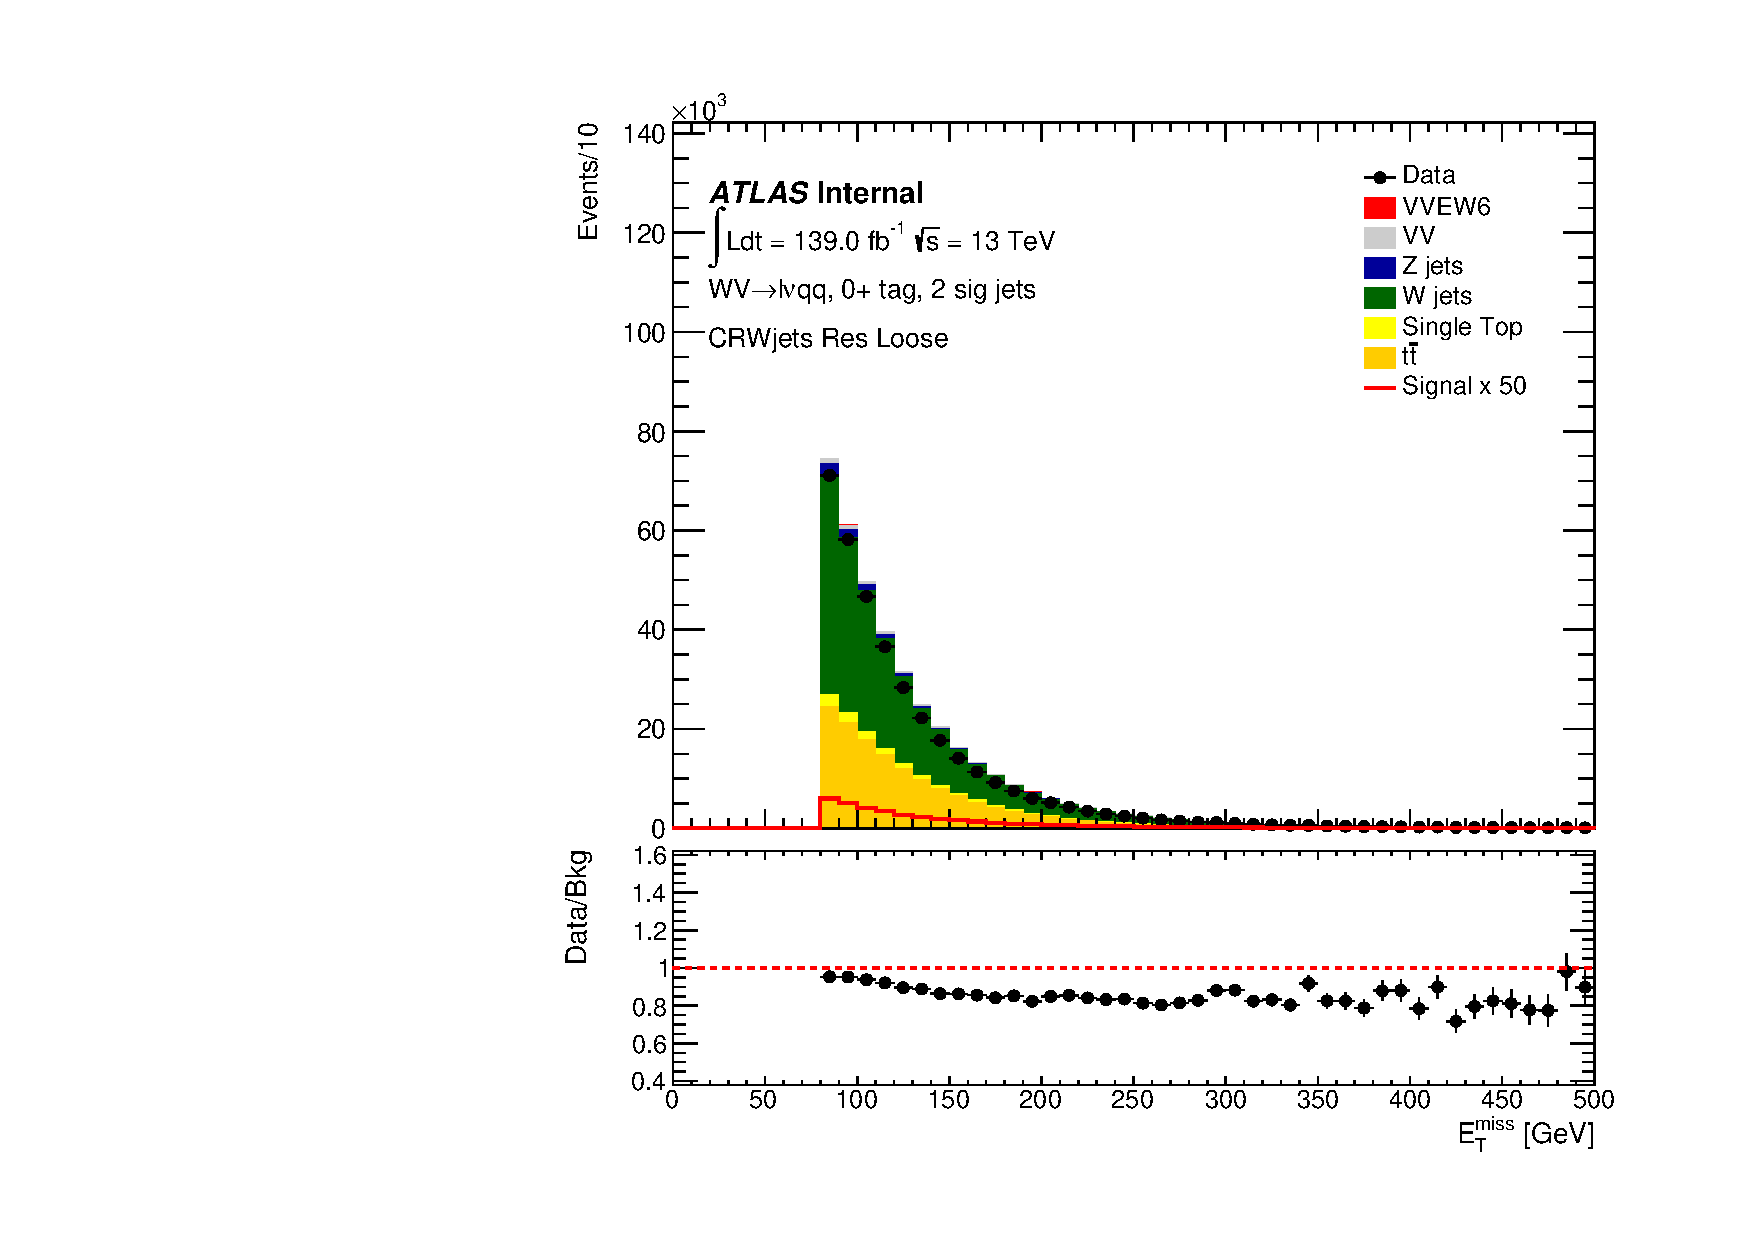
\includegraphics[width=0.3\textwidth]{figures/CRPlots/CRWjets_Res_Loose/stacked_plot_met.pdf}}  %%\\
%%    \subfloat[]{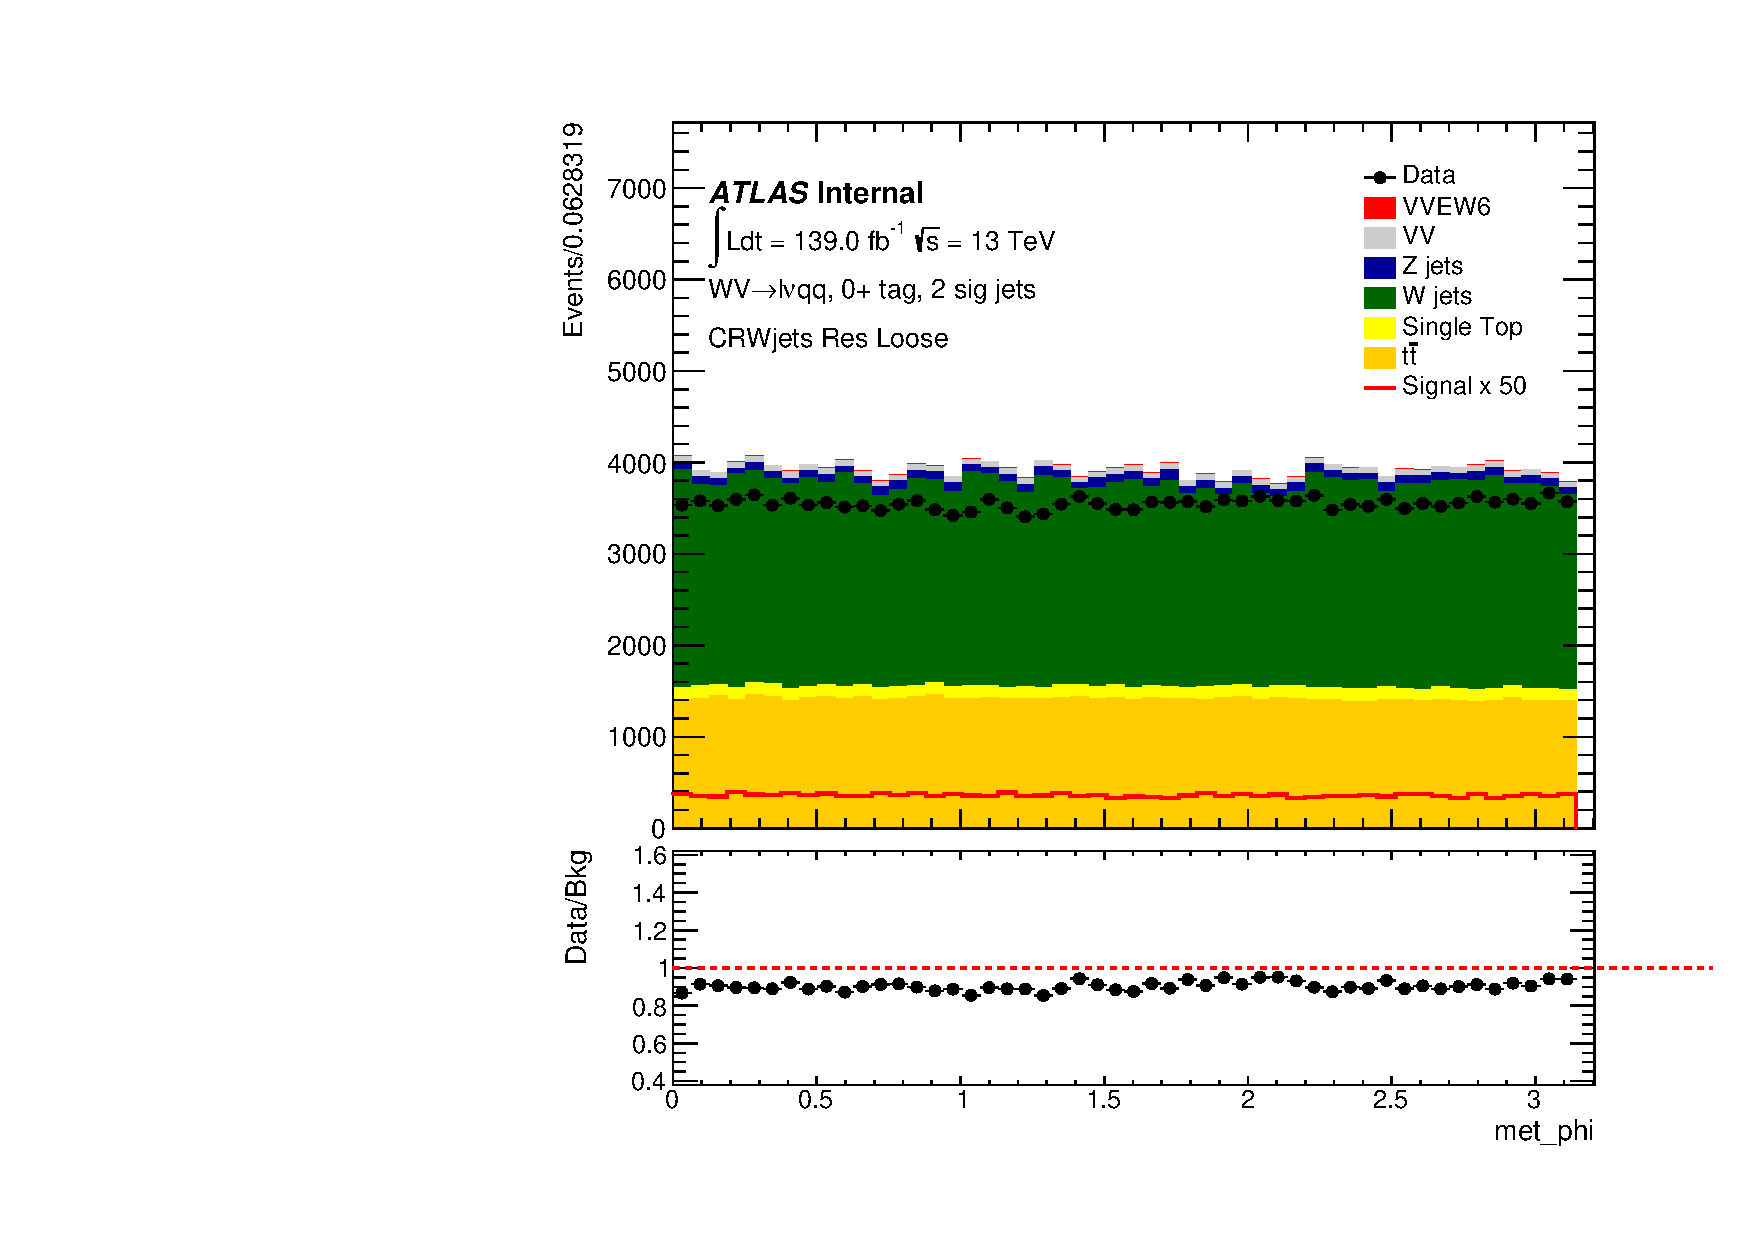
\includegraphics[width=0.3\textwidth]{figures/CRPlots/CRWjets_Res_Loose/stacked_plot_met_phi.pdf}}
%%    \subfloat[]{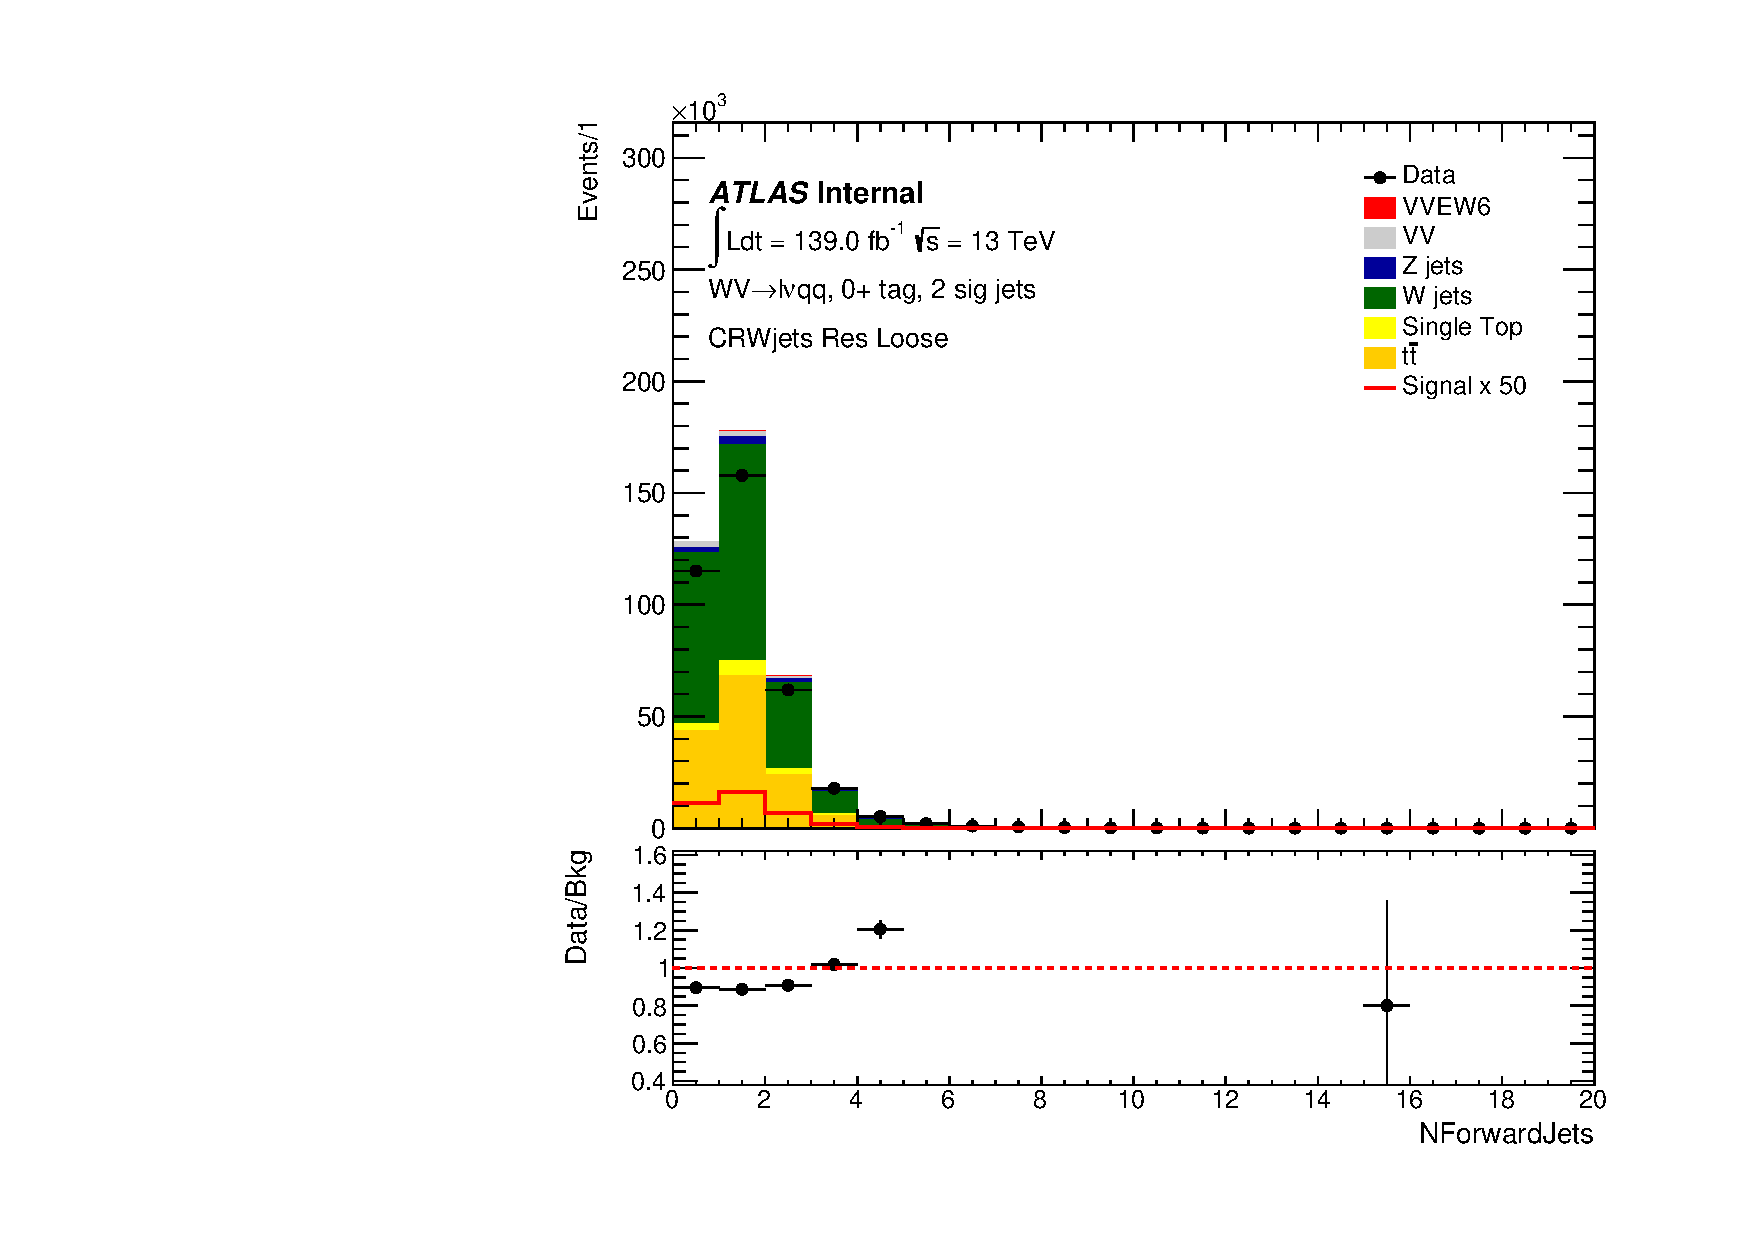
\includegraphics[width=0.3\textwidth]{figures/CRPlots/CRWjets_Res_Loose/stacked_plot_NForwardJets.pdf}}
    \caption{Data-MC checks for the resolved loose \Wjets control region in the \olep channel.}
    \label{fig:CRWjetResLoosePlots1Lep2}
\end{figure}

\begin{figure}[ht]
    \centering
    \subfloat[]{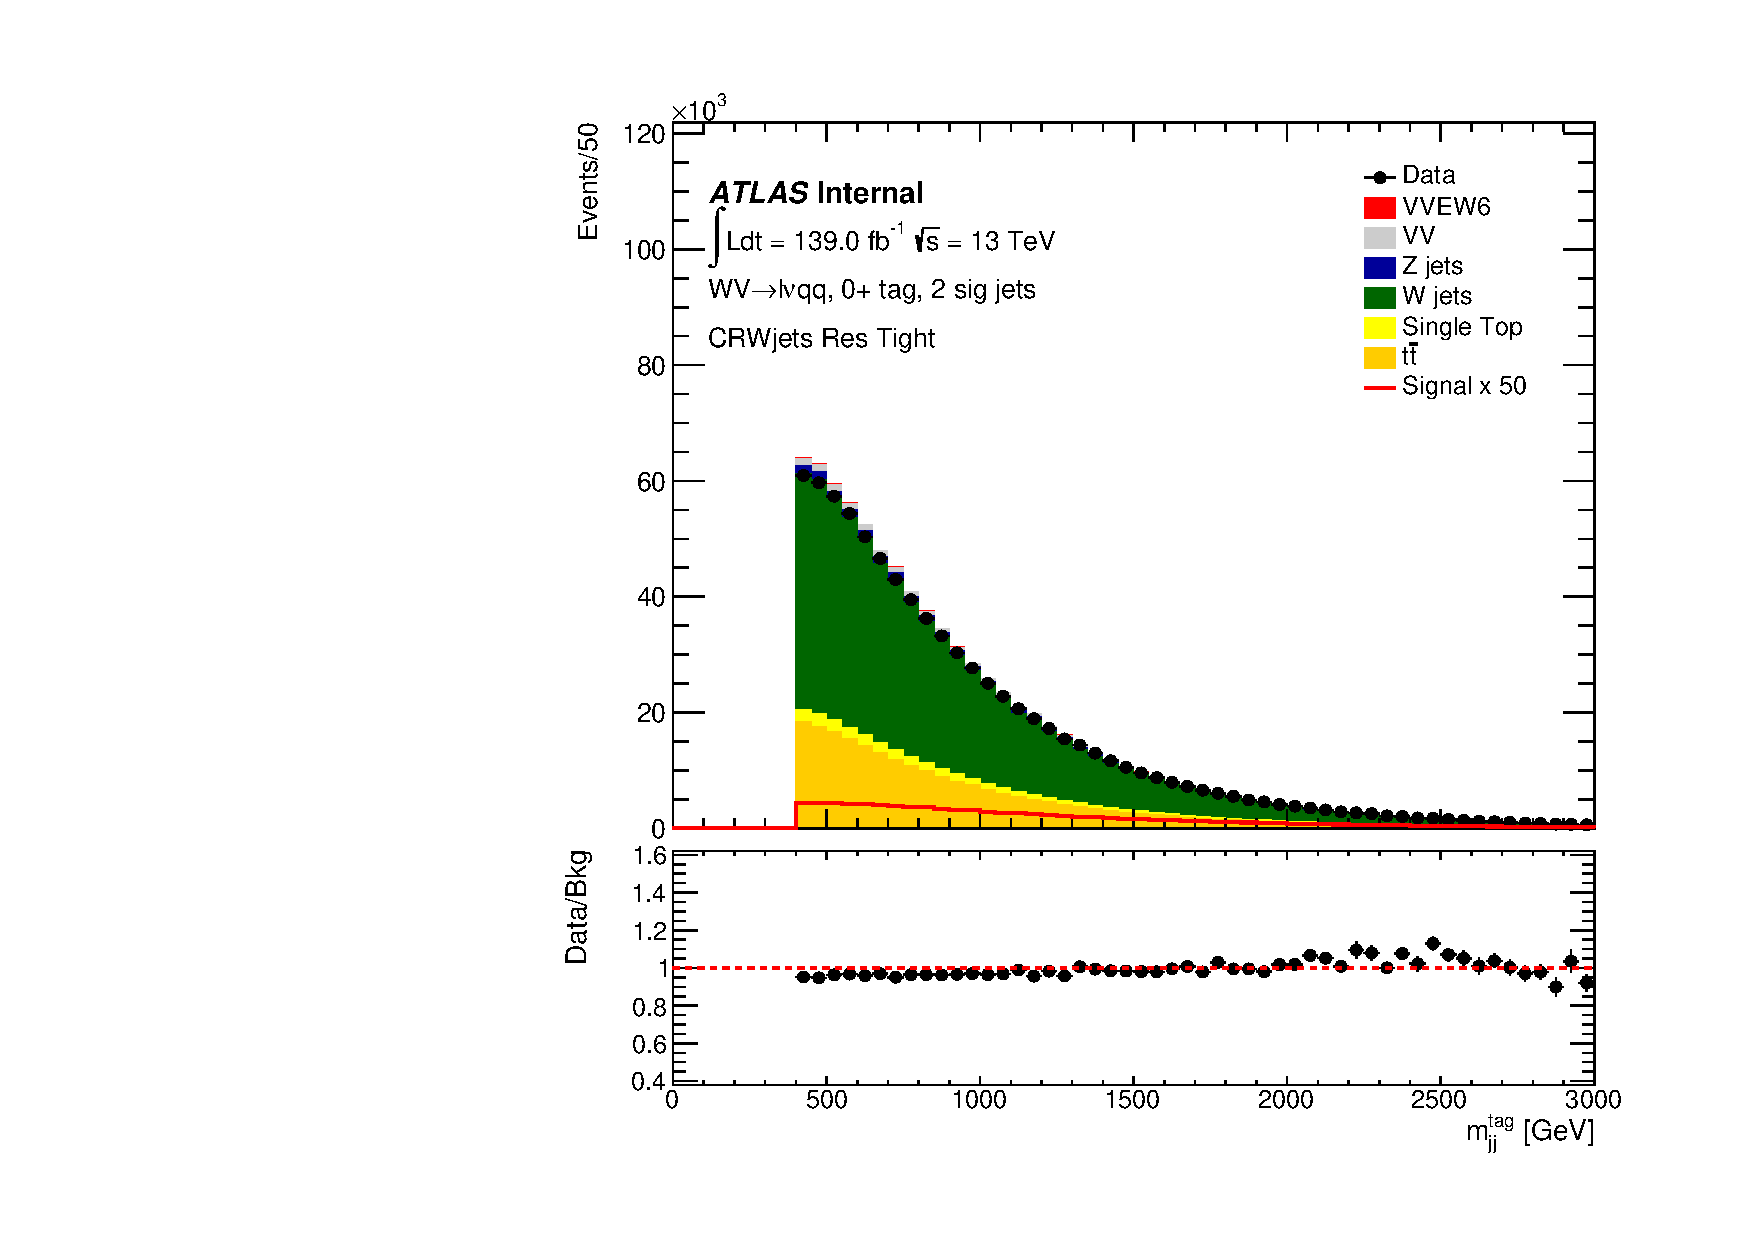
\includegraphics[width=0.3\textwidth]{figures/CRPlots/CRWjets_Res_Tight/stacked_plot_resolved_tagMjj.pdf}}
    \subfloat[]{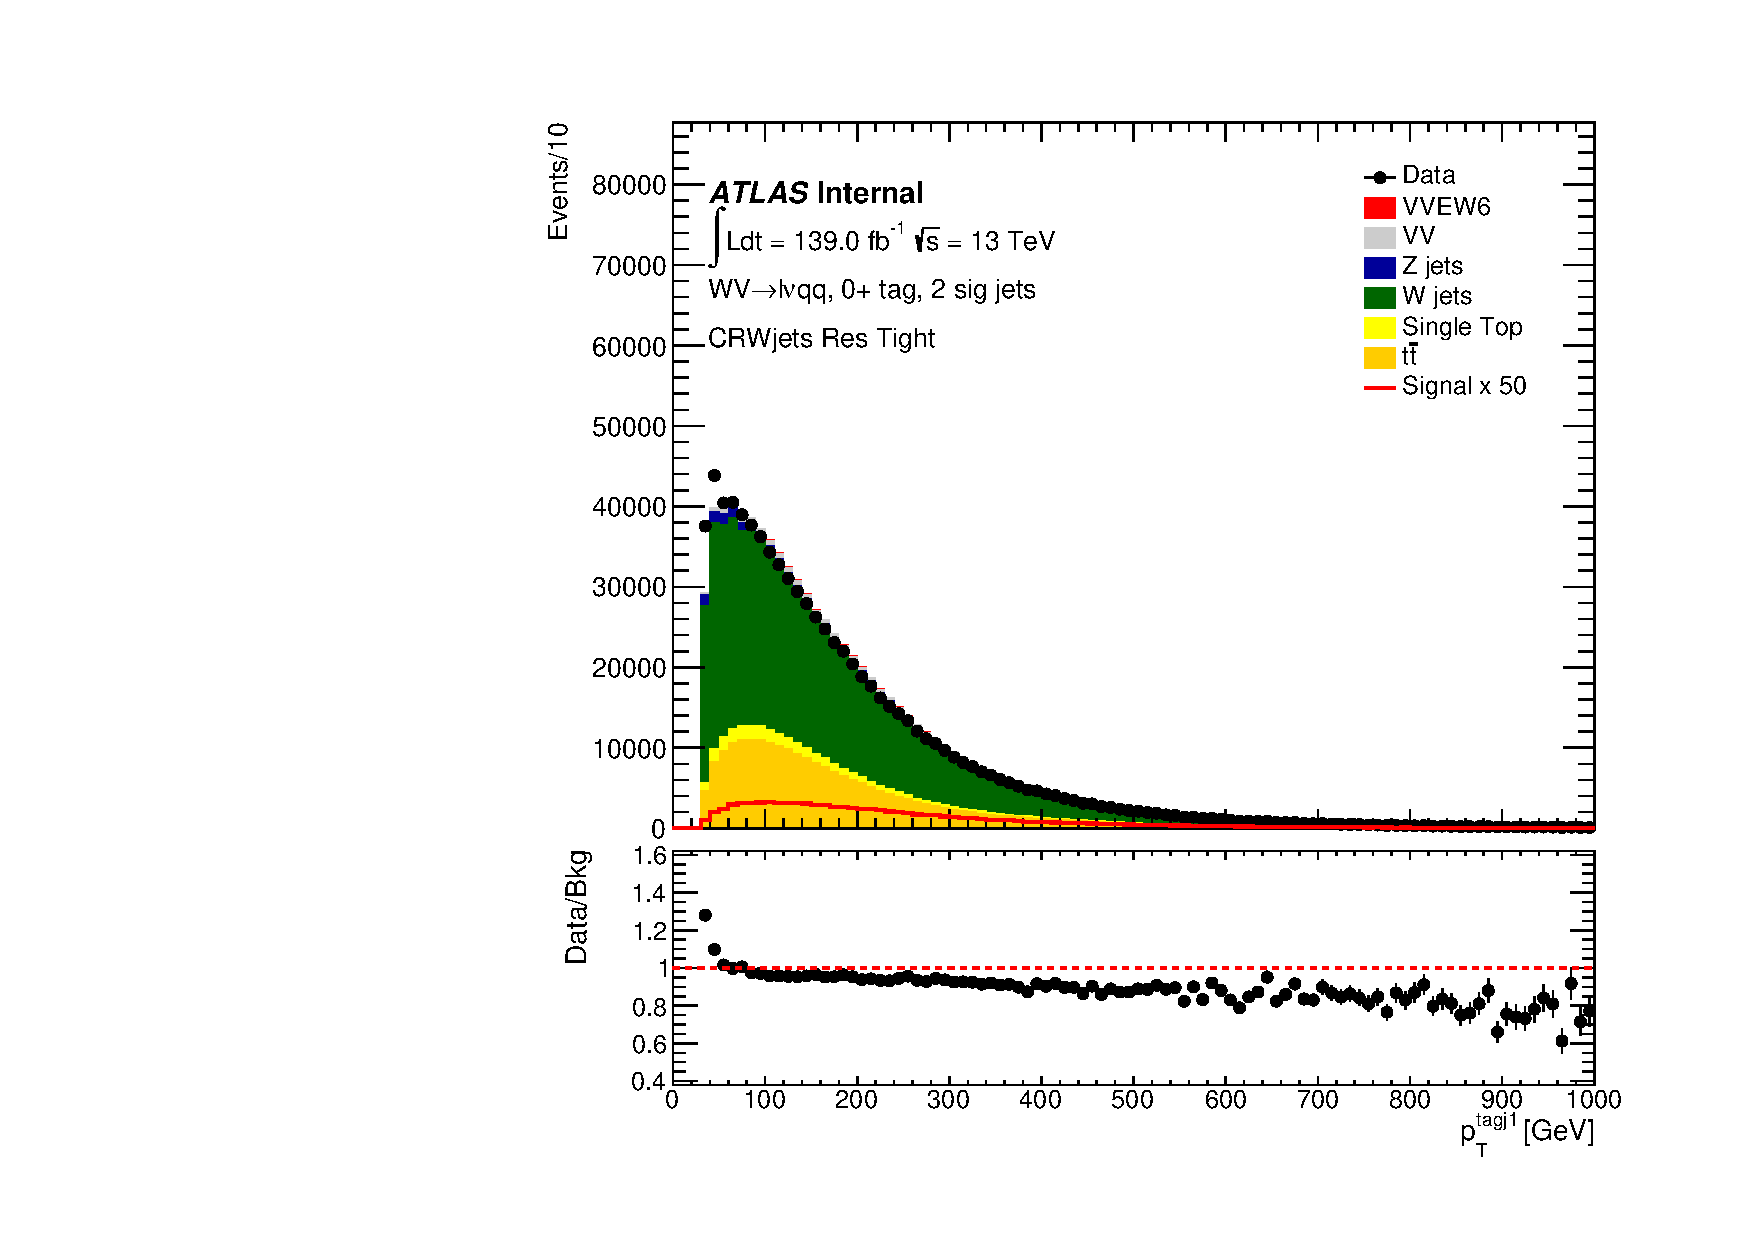
\includegraphics[width=0.3\textwidth]{figures/CRPlots/CRWjets_Res_Tight/stacked_plot_resolved_tagJ1_pt.pdf}}
    \subfloat[]{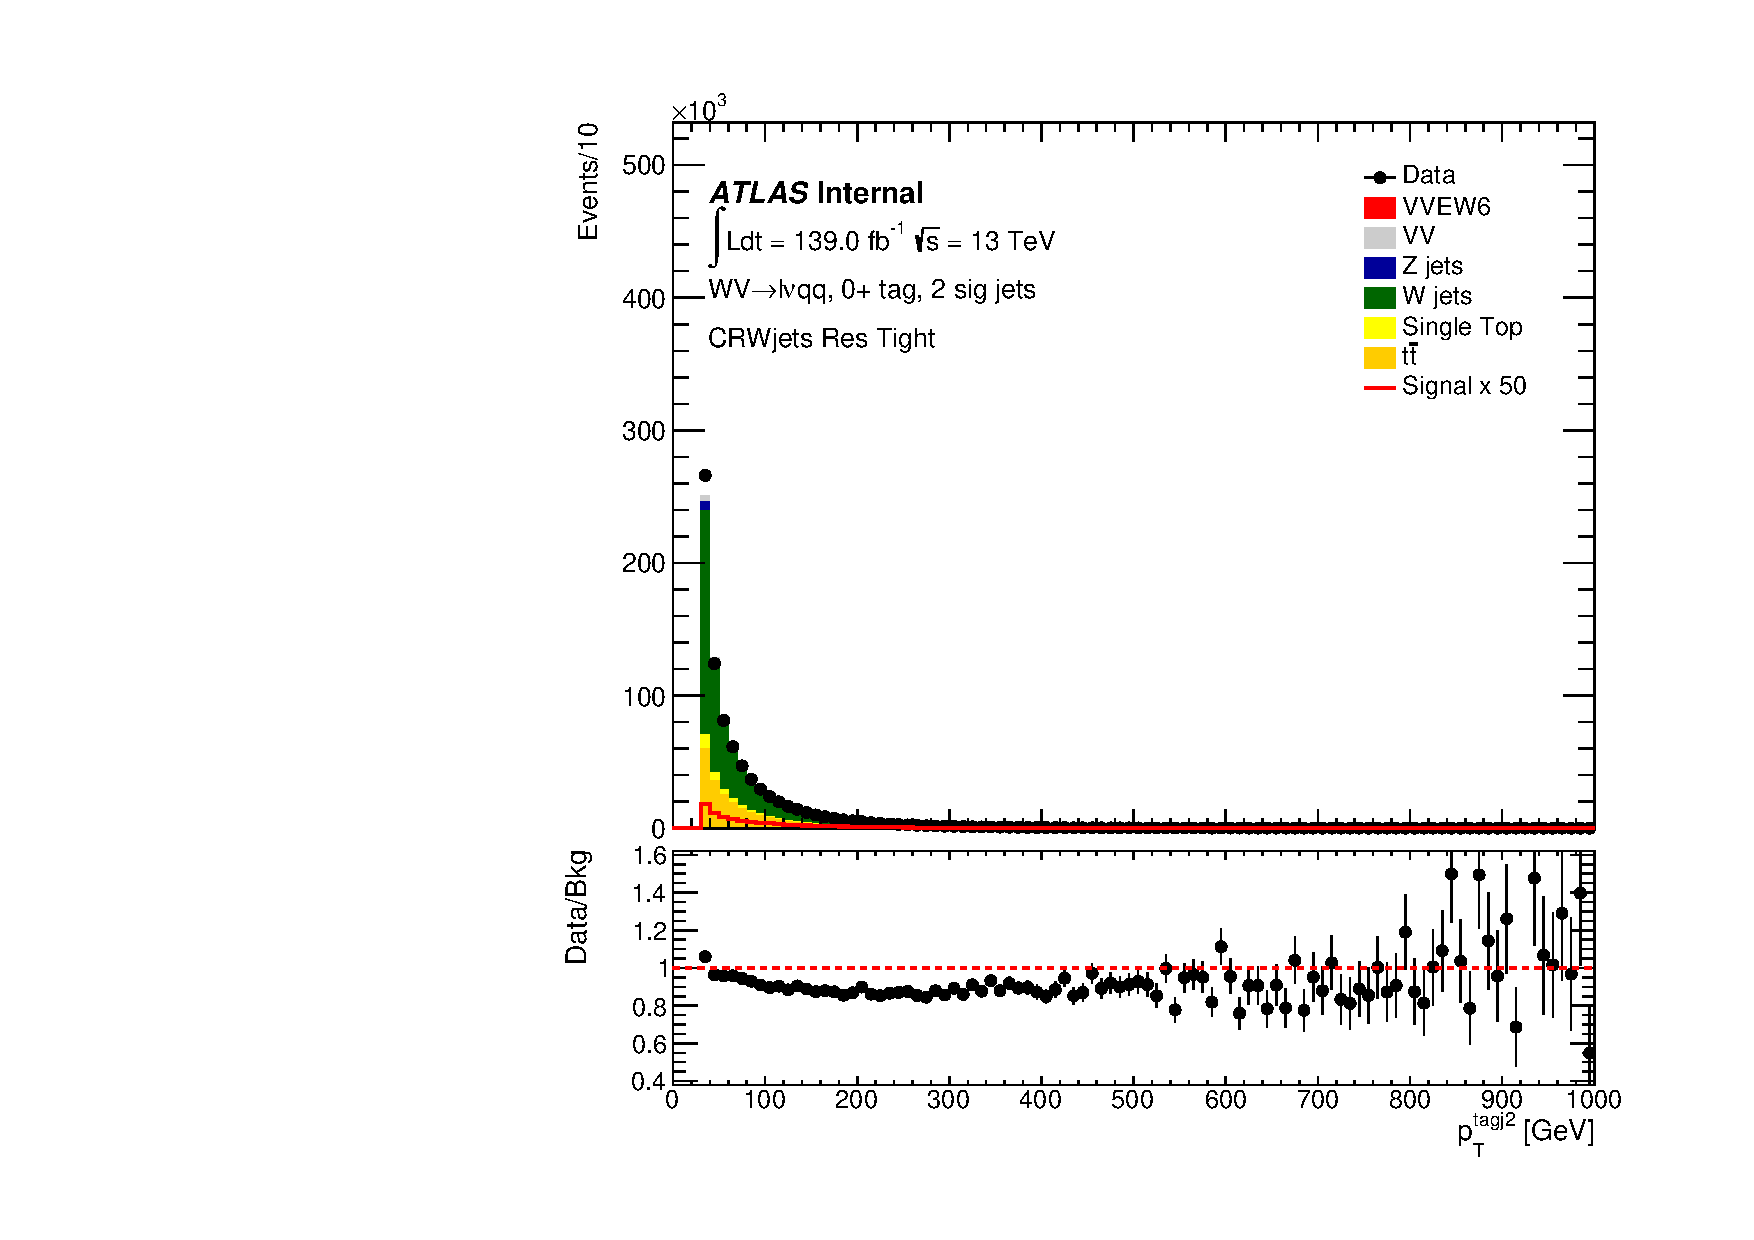
\includegraphics[width=0.3\textwidth]{figures/CRPlots/CRWjets_Res_Tight/stacked_plot_resolved_tagJ2_pt.pdf}} \\
    \subfloat[]{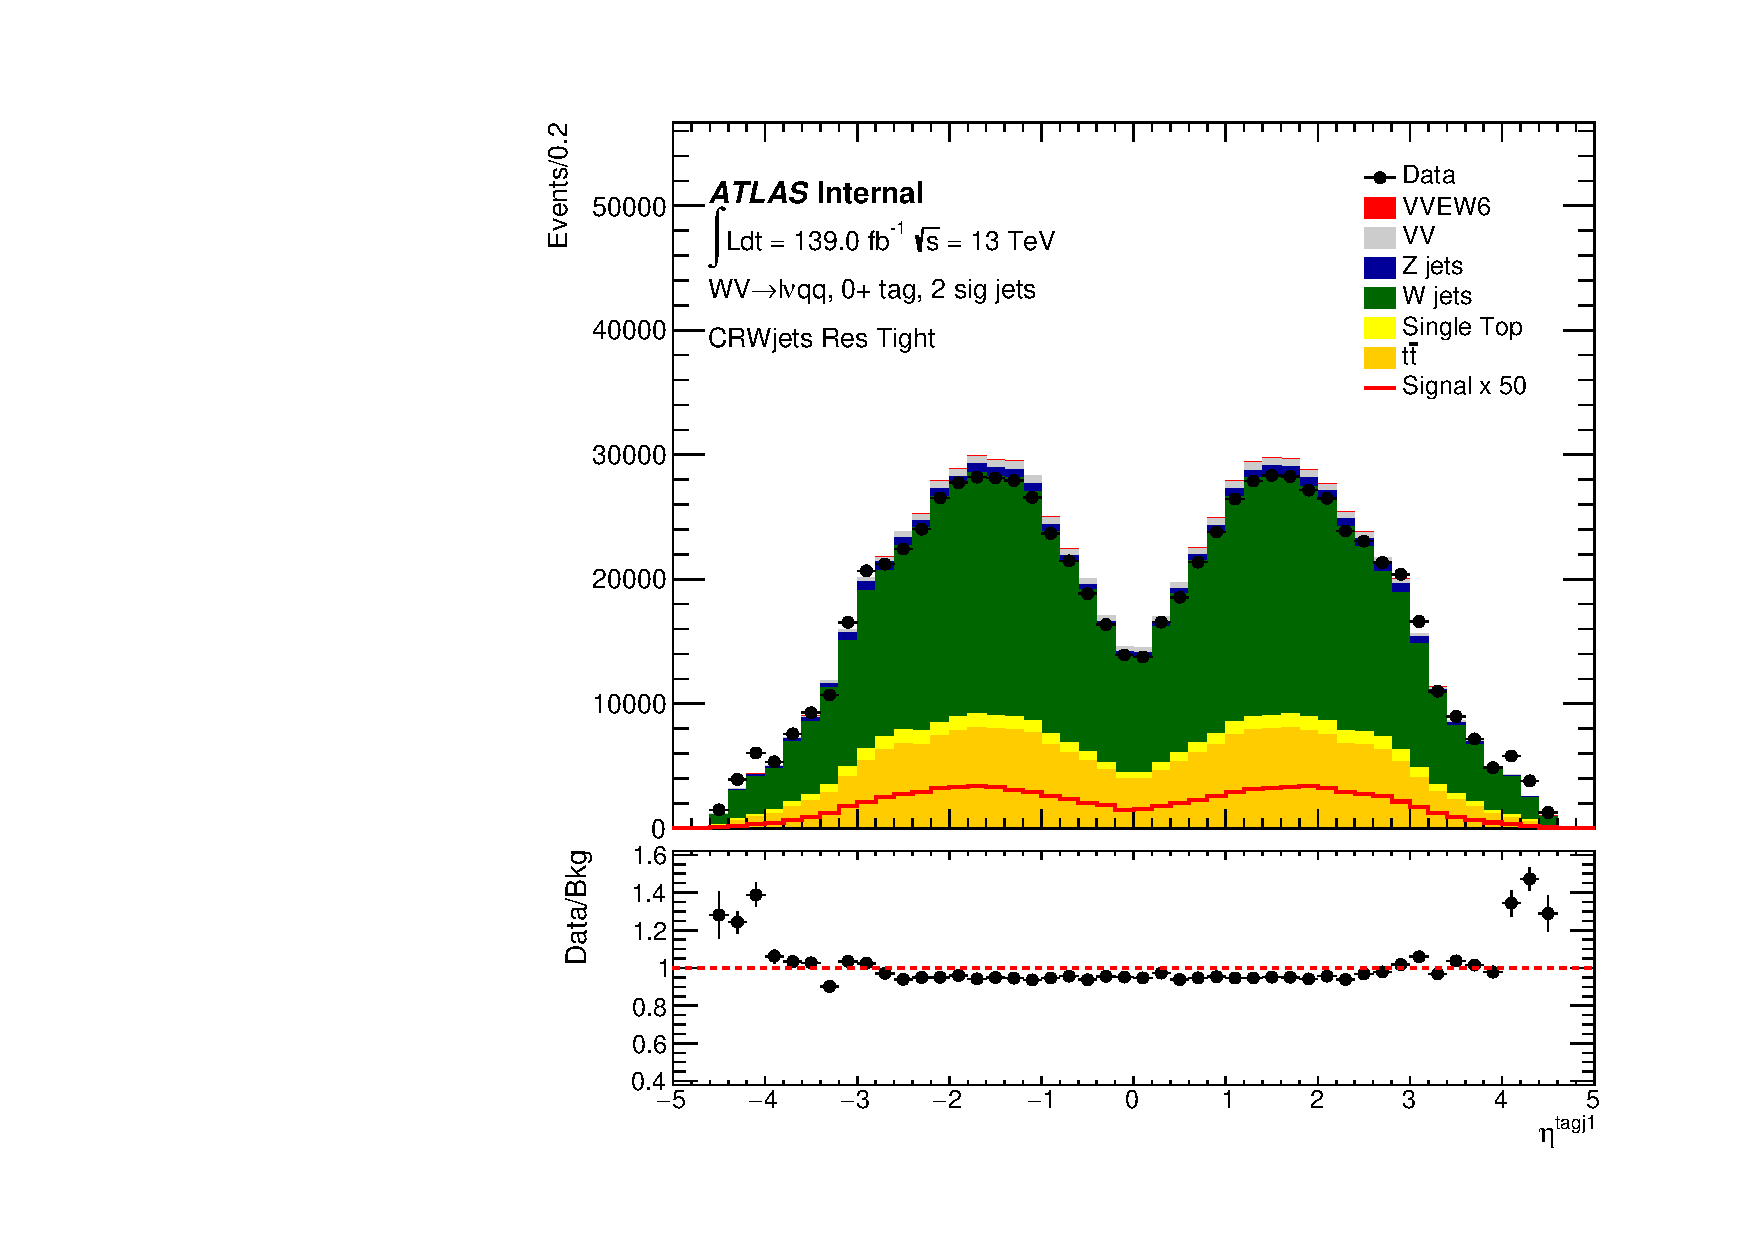
\includegraphics[width=0.3\textwidth]{figures/CRPlots/CRWjets_Res_Tight/stacked_plot_resolved_tagJ1_eta.pdf}}
    \subfloat[]{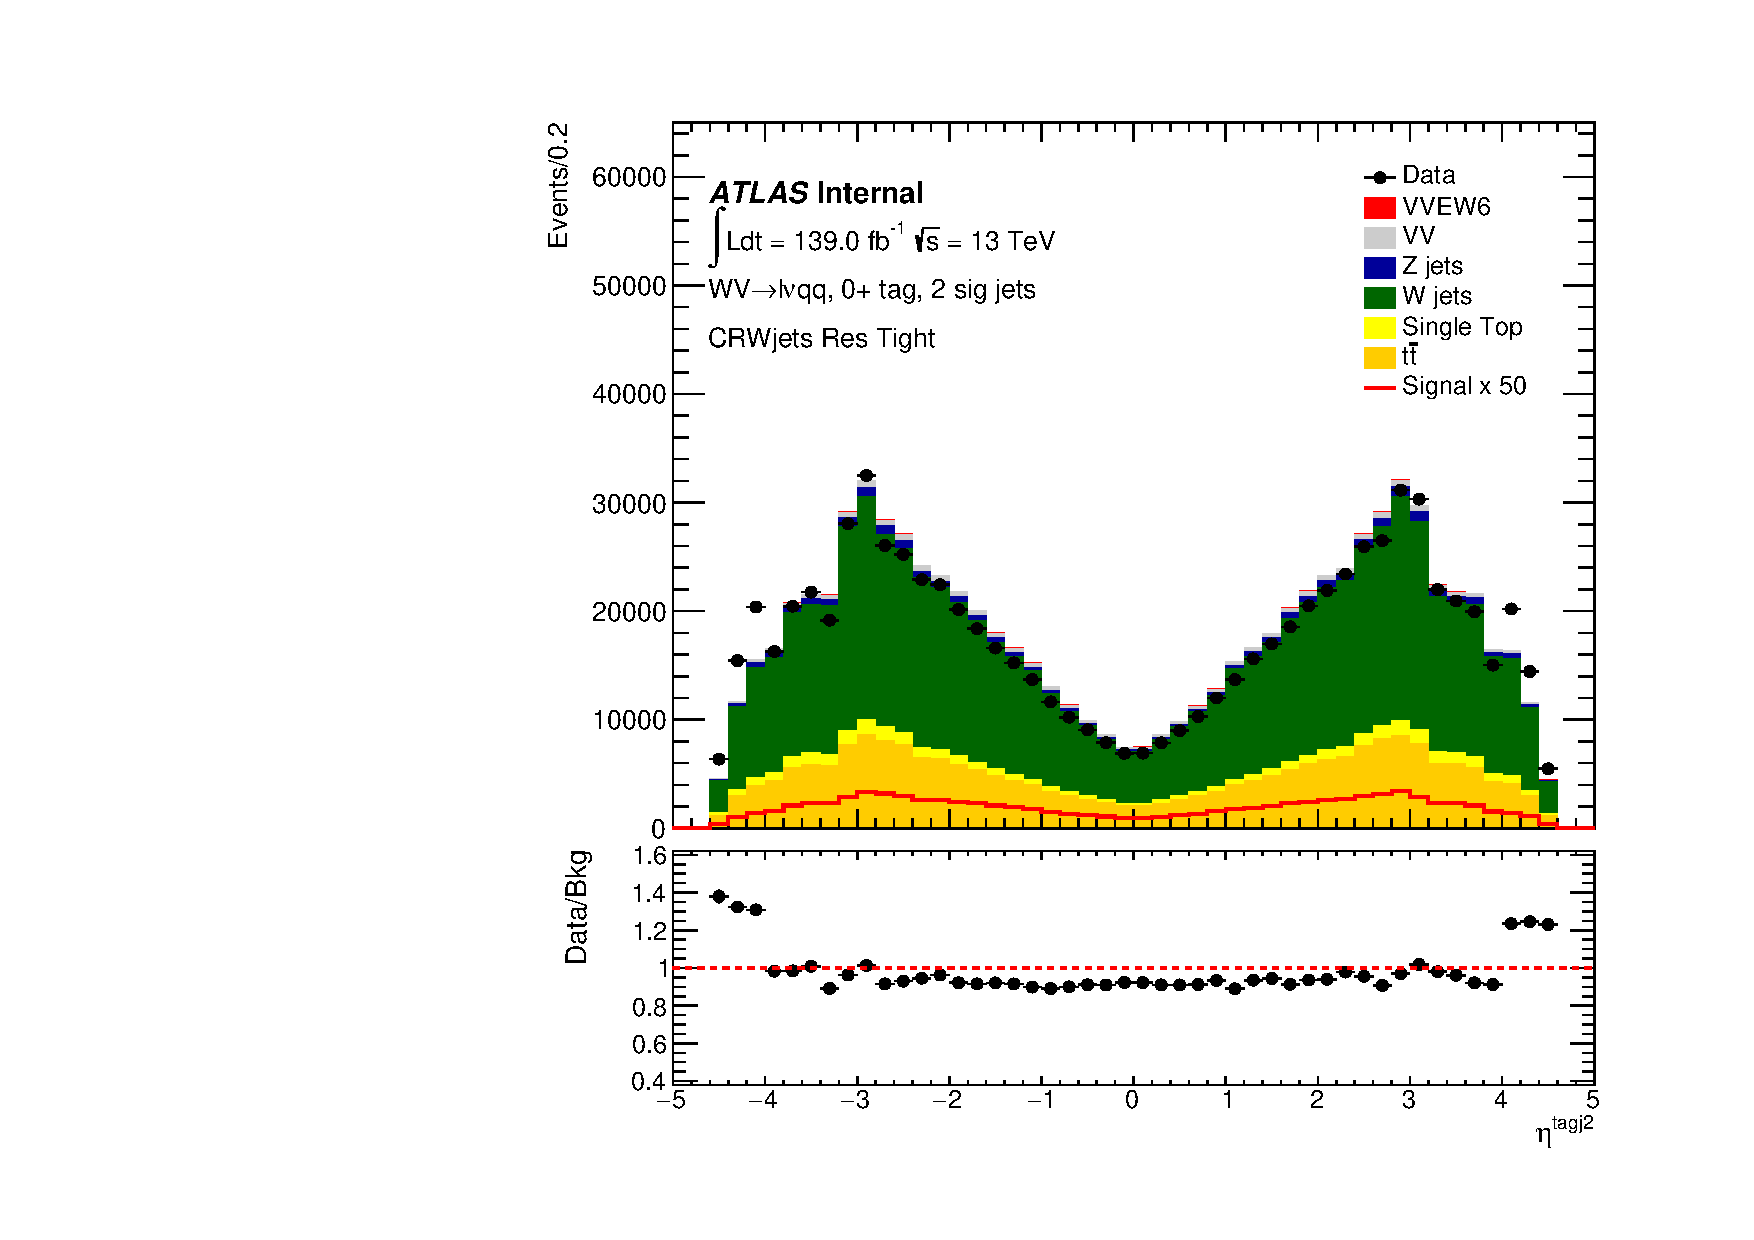
\includegraphics[width=0.3\textwidth]{figures/CRPlots/CRWjets_Res_Tight/stacked_plot_resolved_tagJ2_eta.pdf}} \\
    \subfloat[]{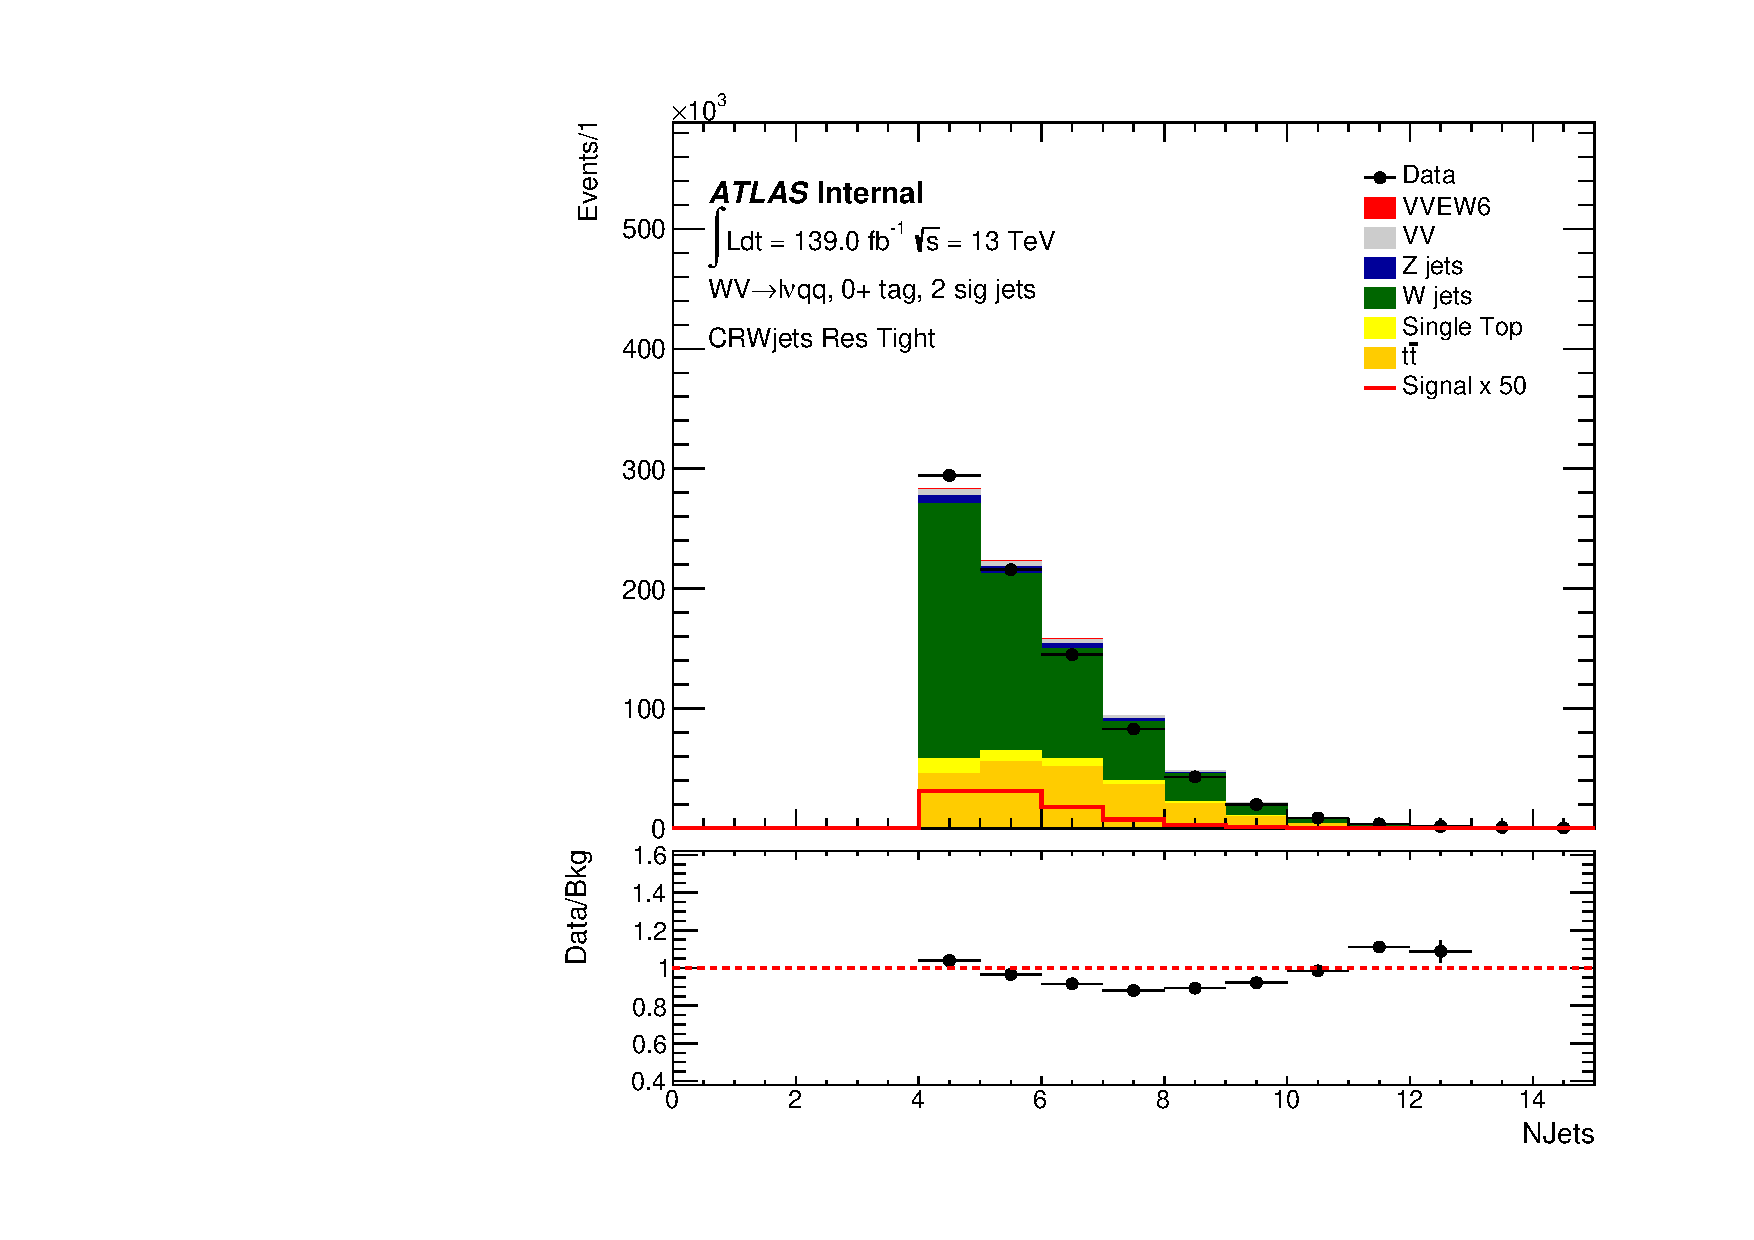
\includegraphics[width=0.3\textwidth]{figures/CRPlots/CRWjets_Res_Tight/stacked_plot_NJets.pdf}}
    \subfloat[]{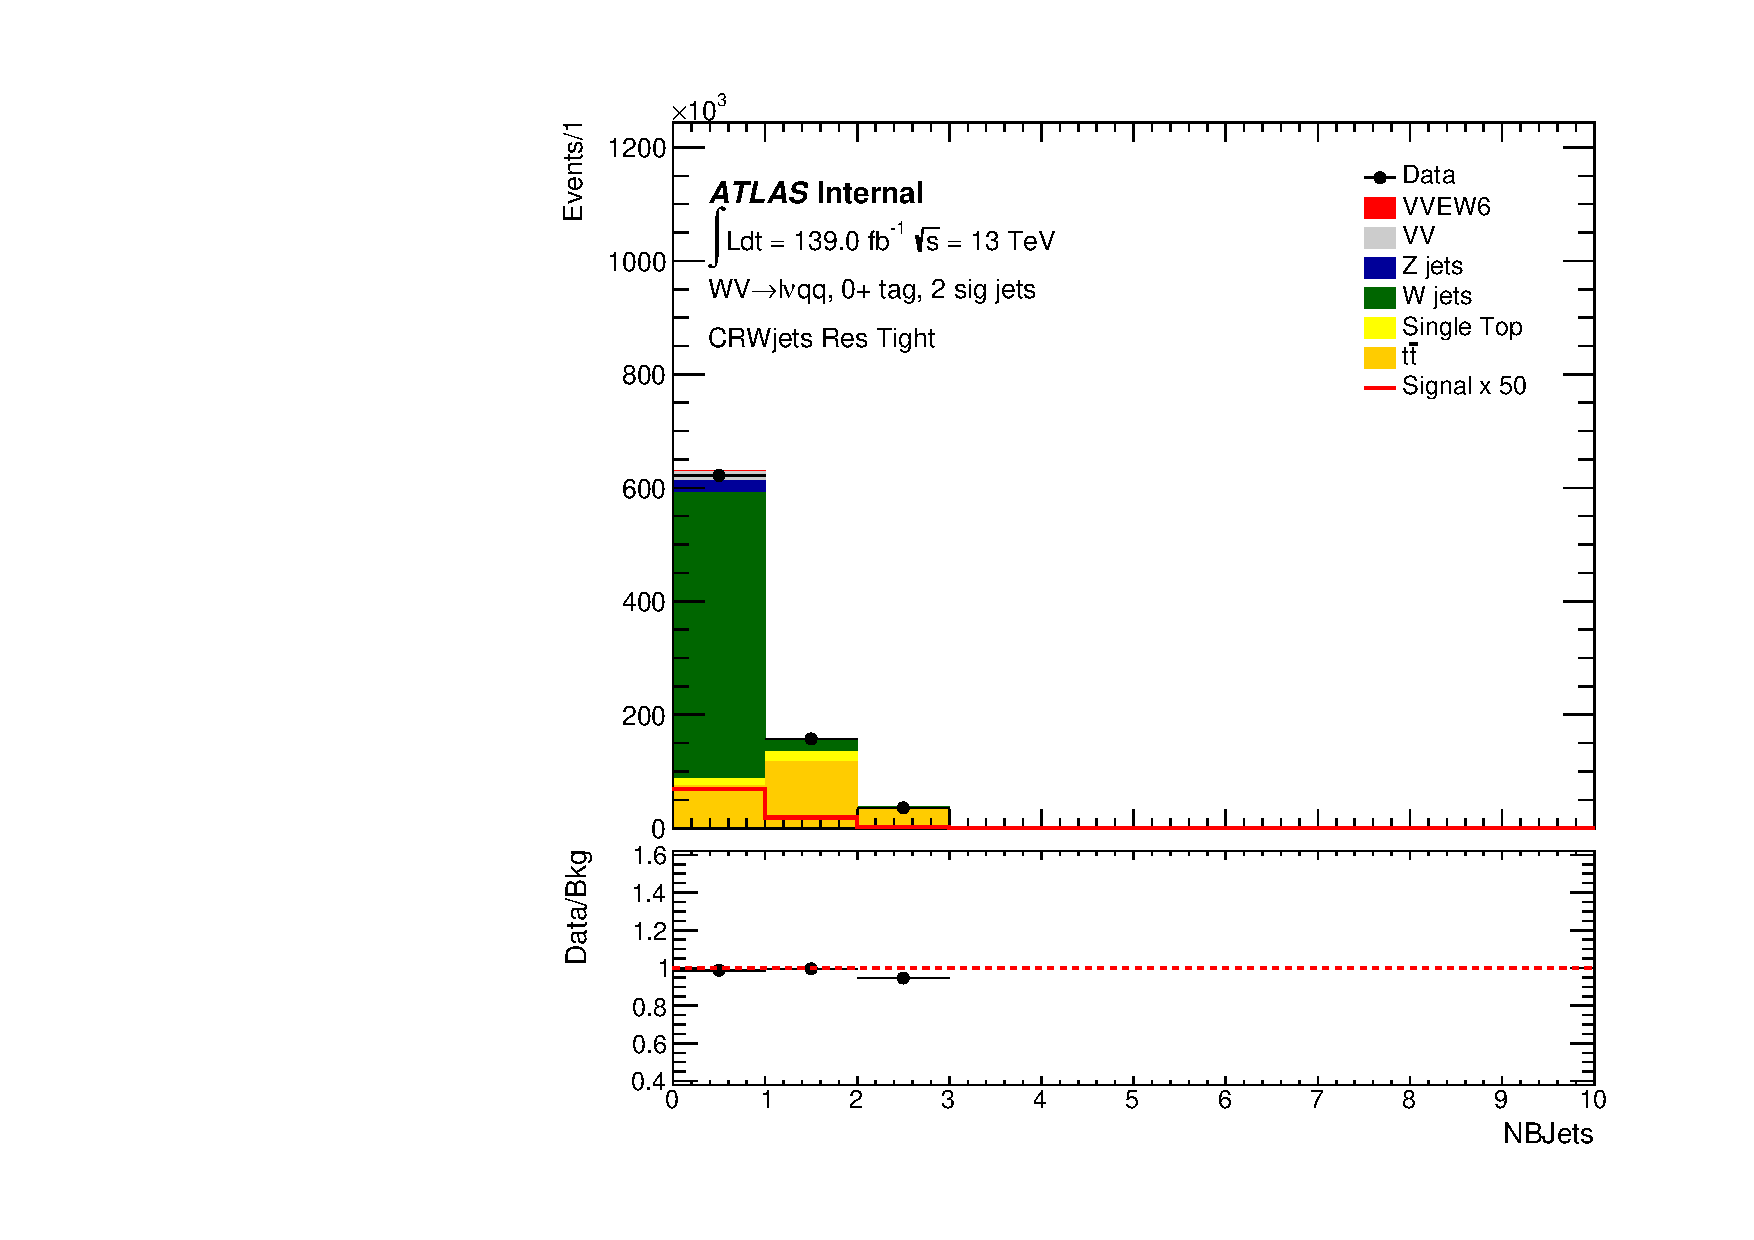
\includegraphics[width=0.3\textwidth]{figures/CRPlots/CRWjets_Res_Tight/stacked_plot_NBJets.pdf}}
    \subfloat[]{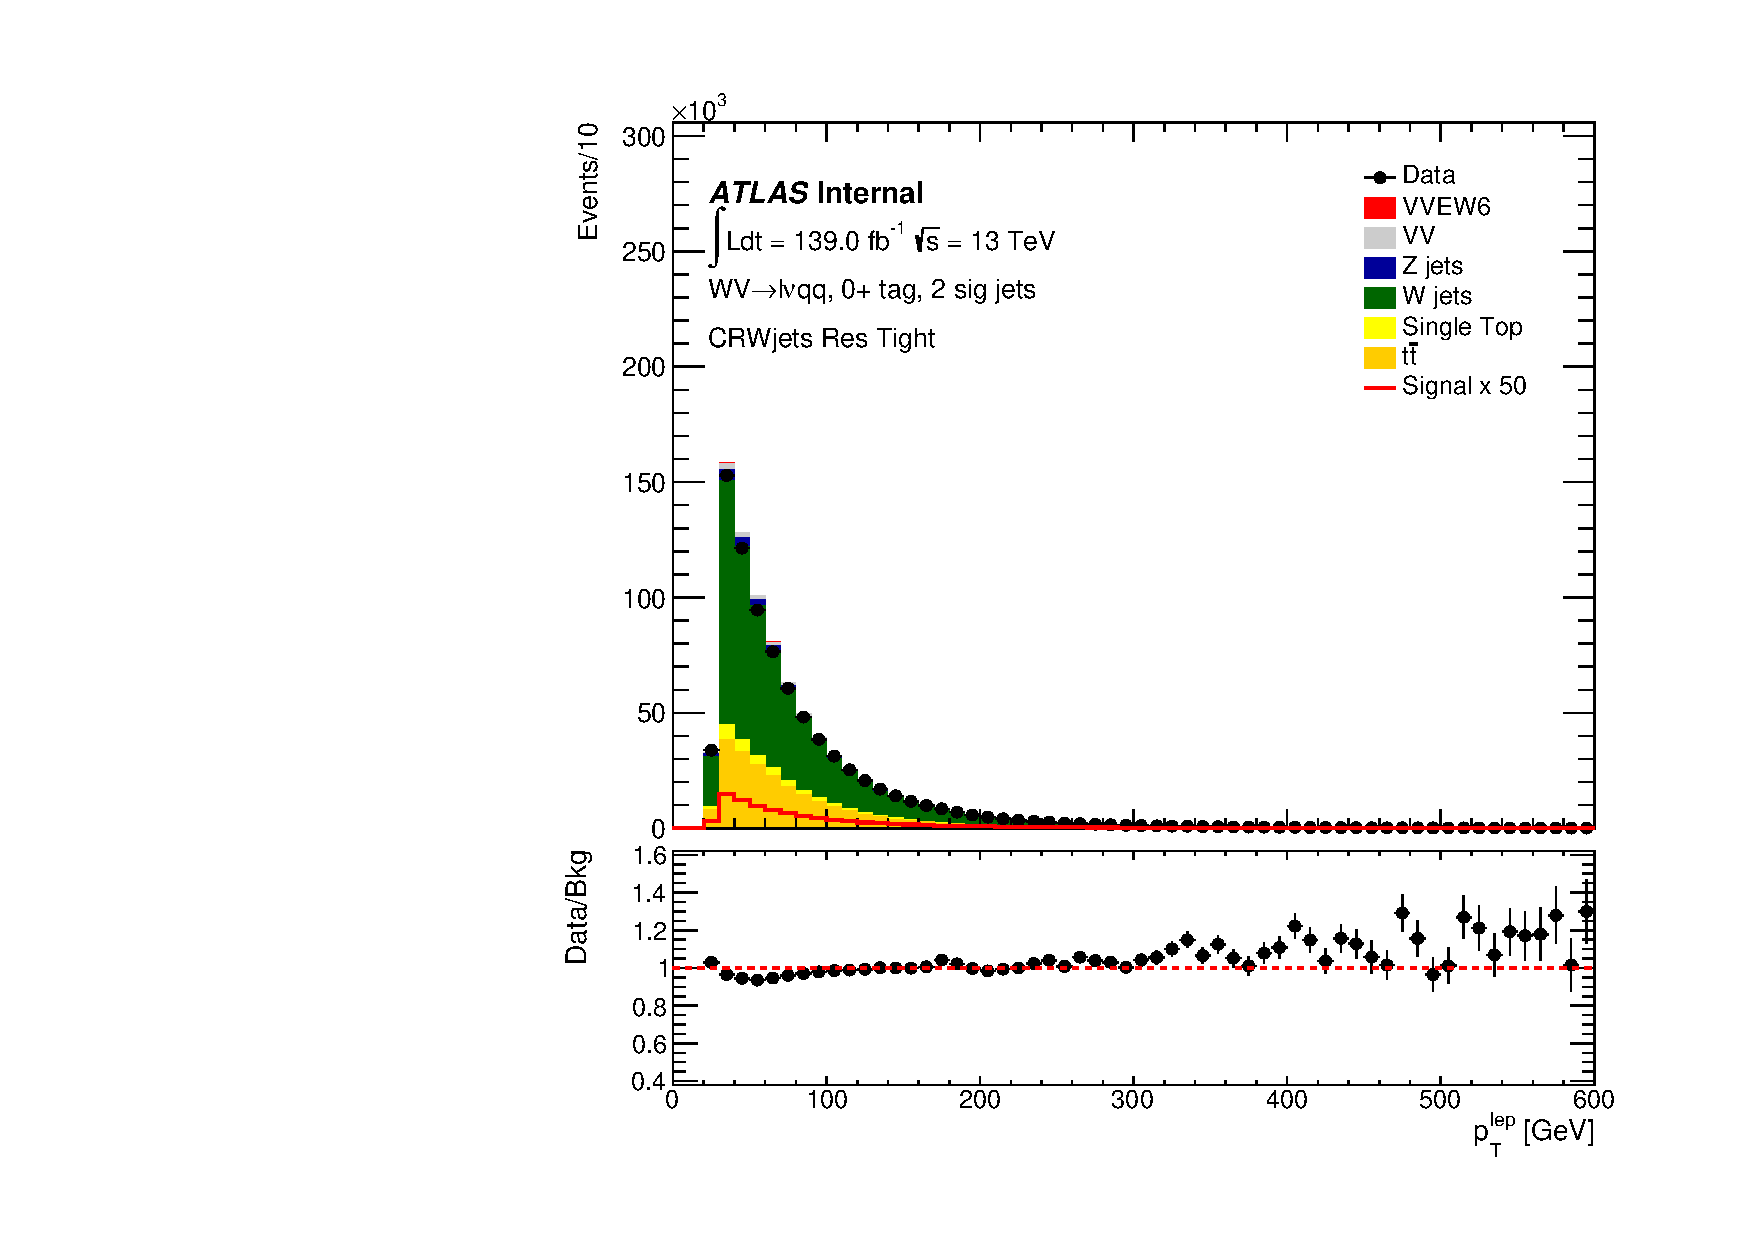
\includegraphics[width=0.3\textwidth]{figures/CRPlots/CRWjets_Res_Tight/stacked_plot_lep_pt.pdf}}  %%\\
    \caption{Data-MC checks for the resolved tight \Wjets control region in the \olep channel.}
    \label{fig:CRWjetResTightPlots1Lep}
\end{figure}


\begin{figure}[ht]
    \centering
    \subfloat[]{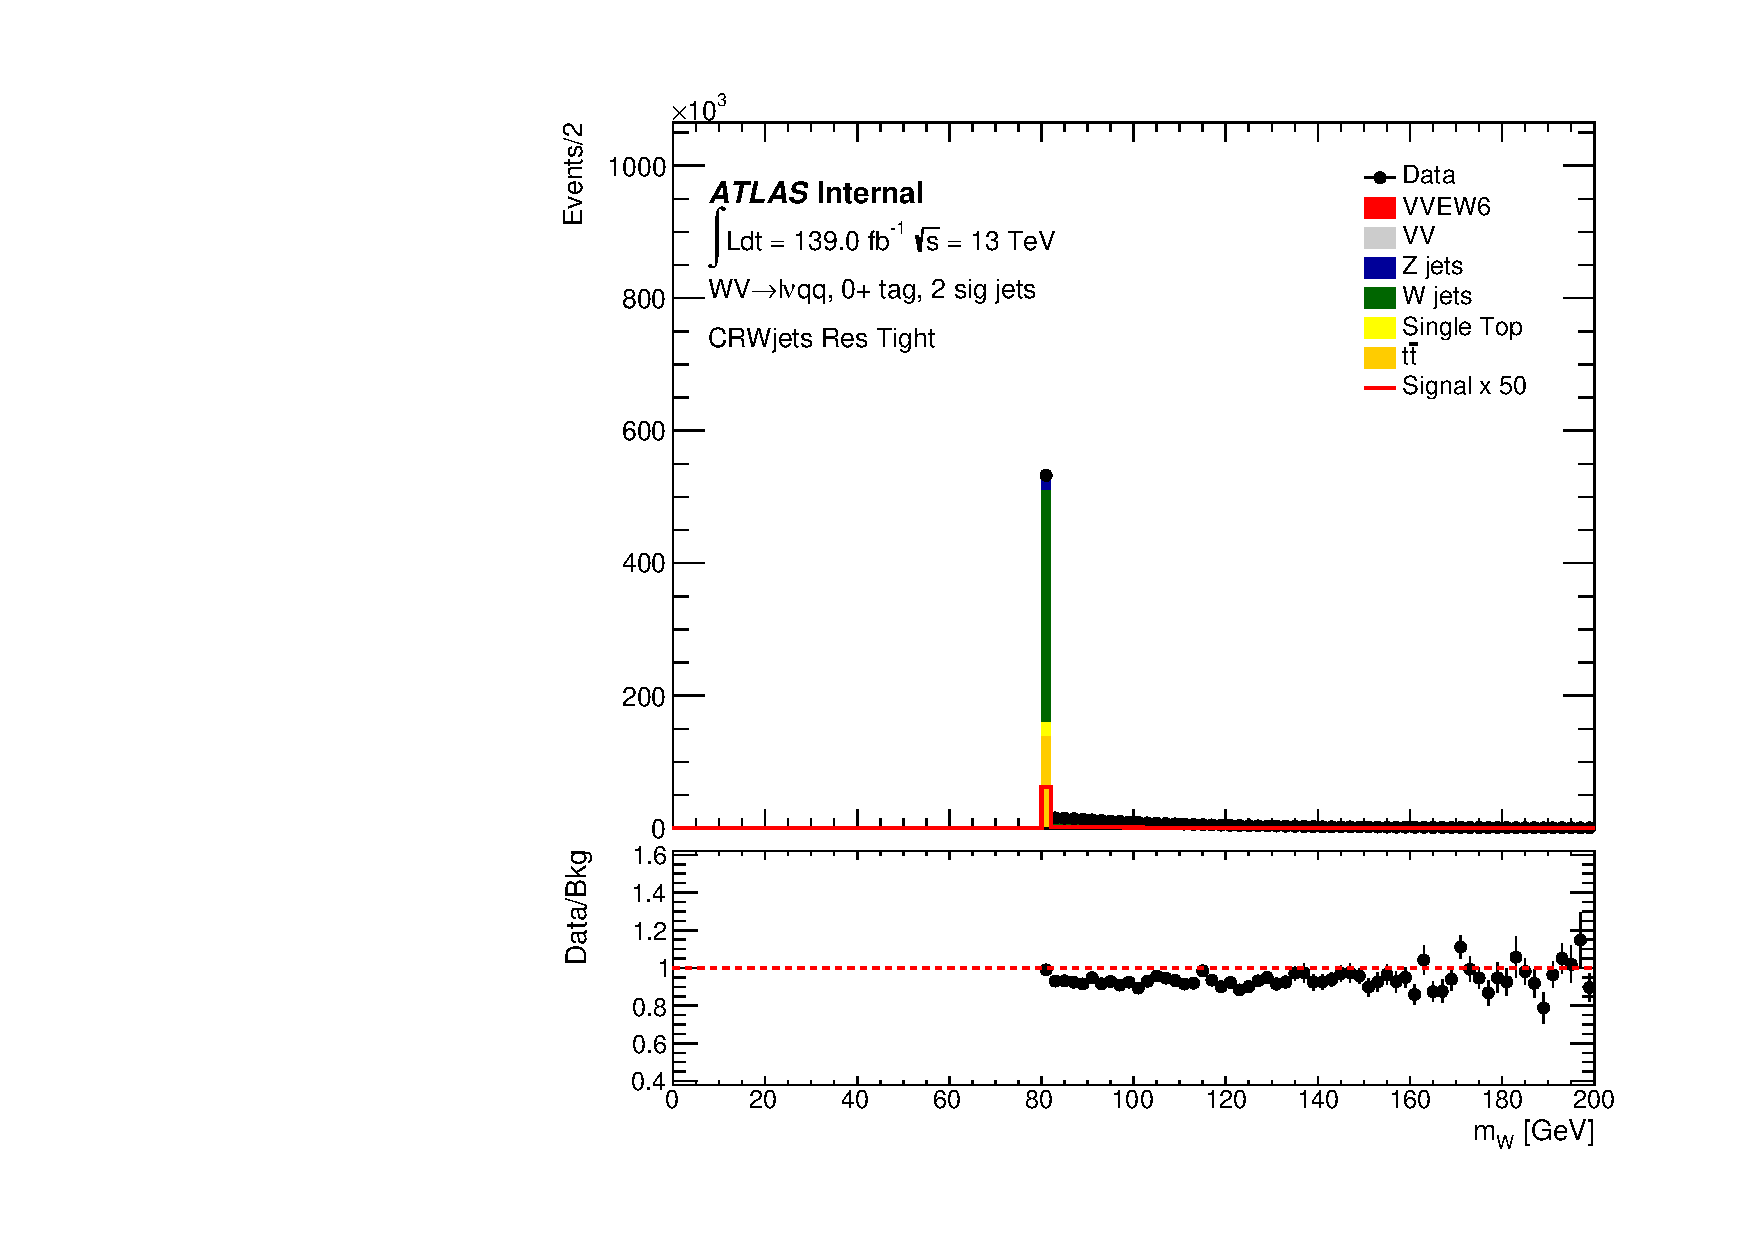
\includegraphics[width=0.3\textwidth]{figures/CRPlots/CRWjets_Res_Tight/stacked_plot_W_m.pdf}}
    \subfloat[]{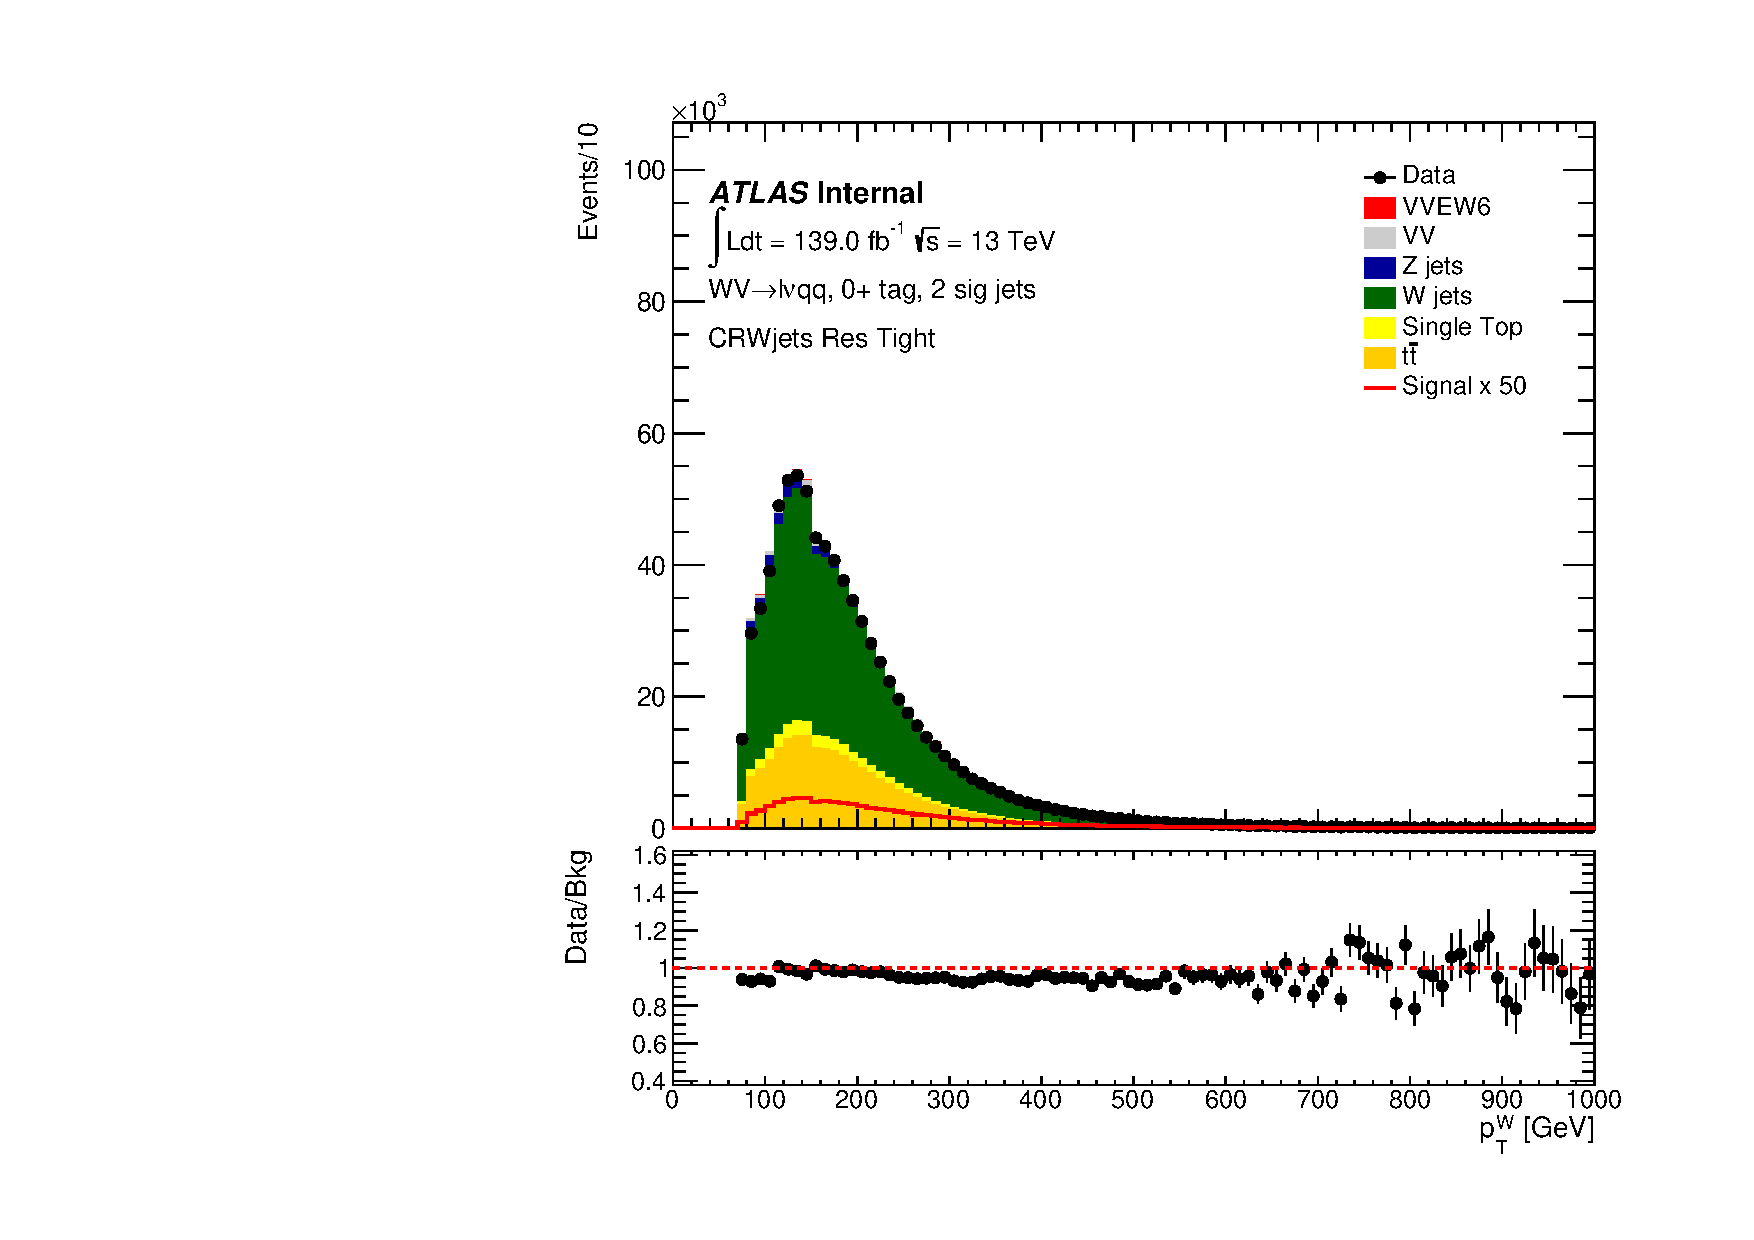
\includegraphics[width=0.3\textwidth]{figures/CRPlots/CRWjets_Res_Tight/stacked_plot_W_pt.pdf}}
    \subfloat[]{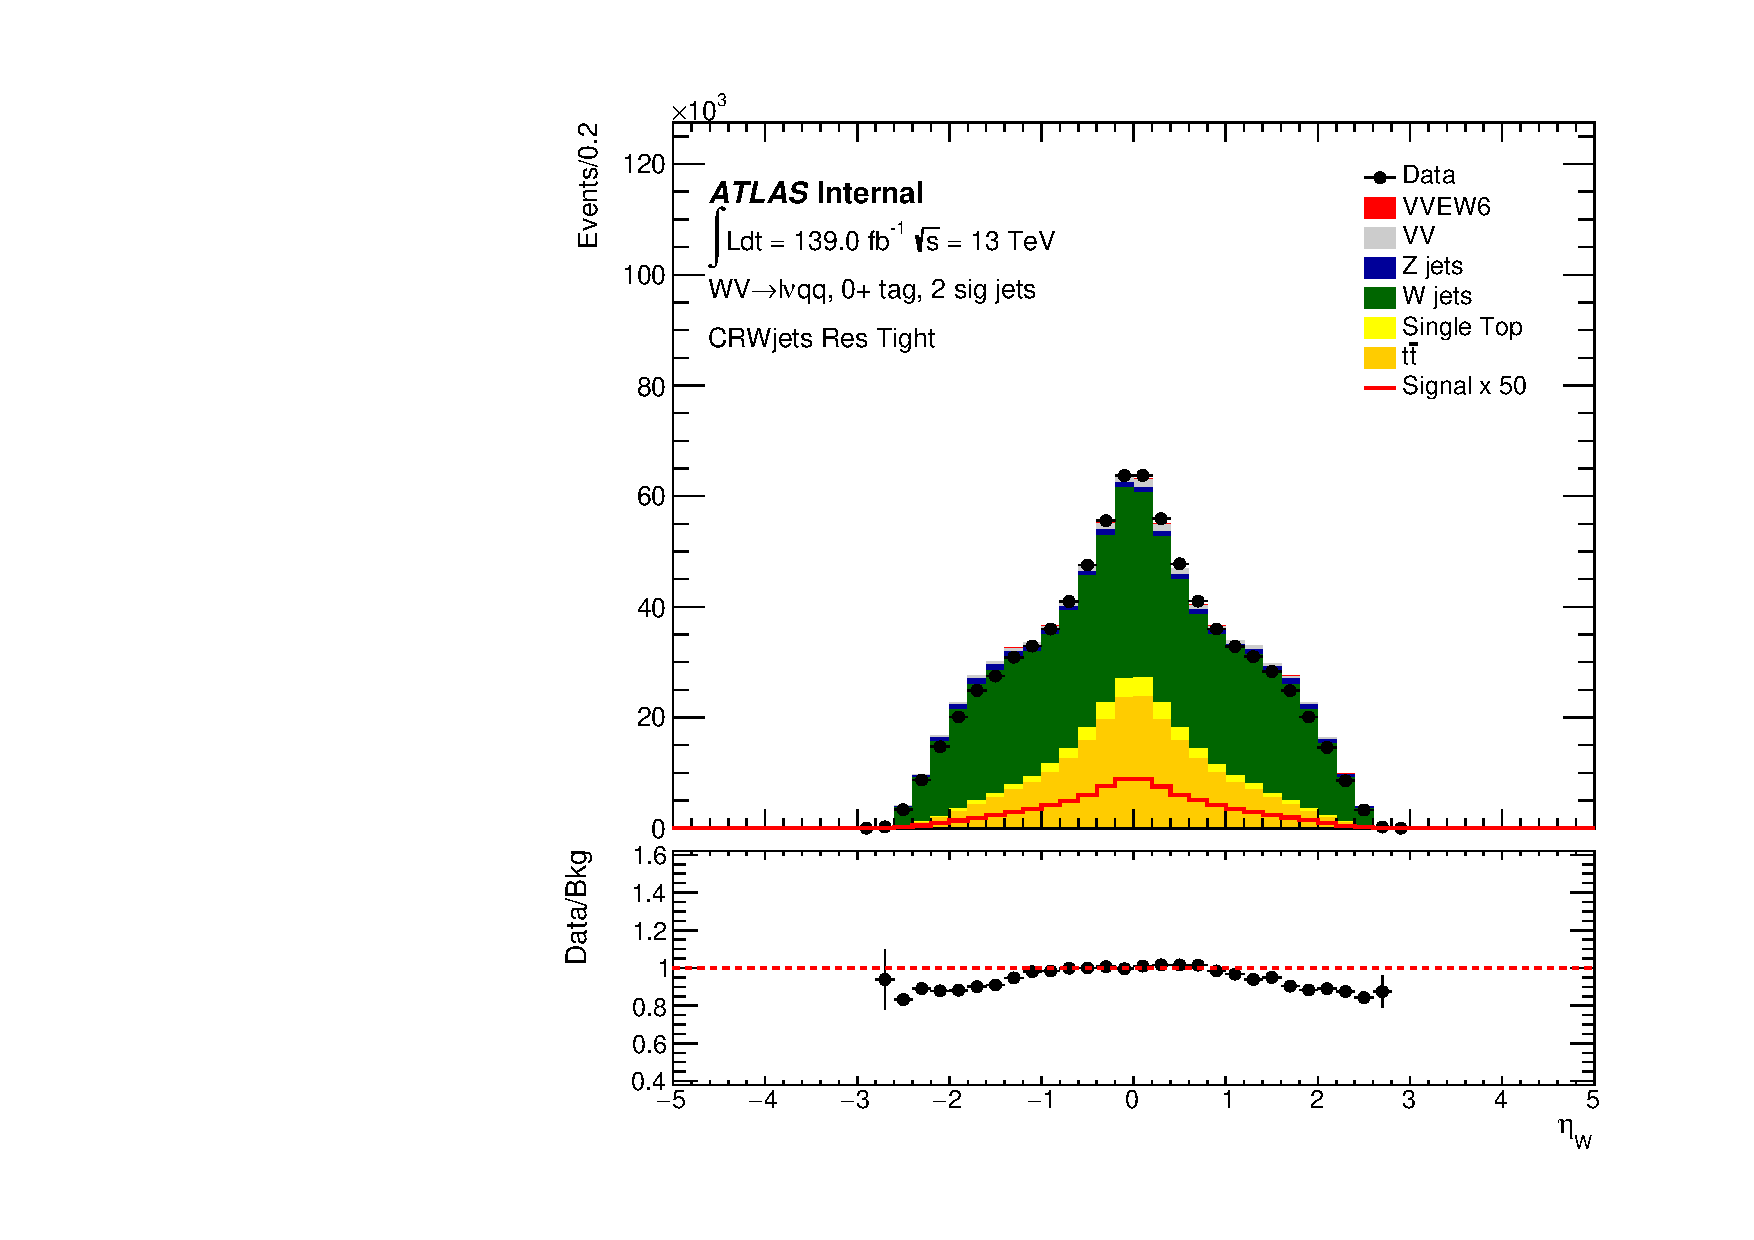
\includegraphics[width=0.3\textwidth]{figures/CRPlots/CRWjets_Res_Tight/stacked_plot_W_eta.pdf}} \\
    \subfloat[]{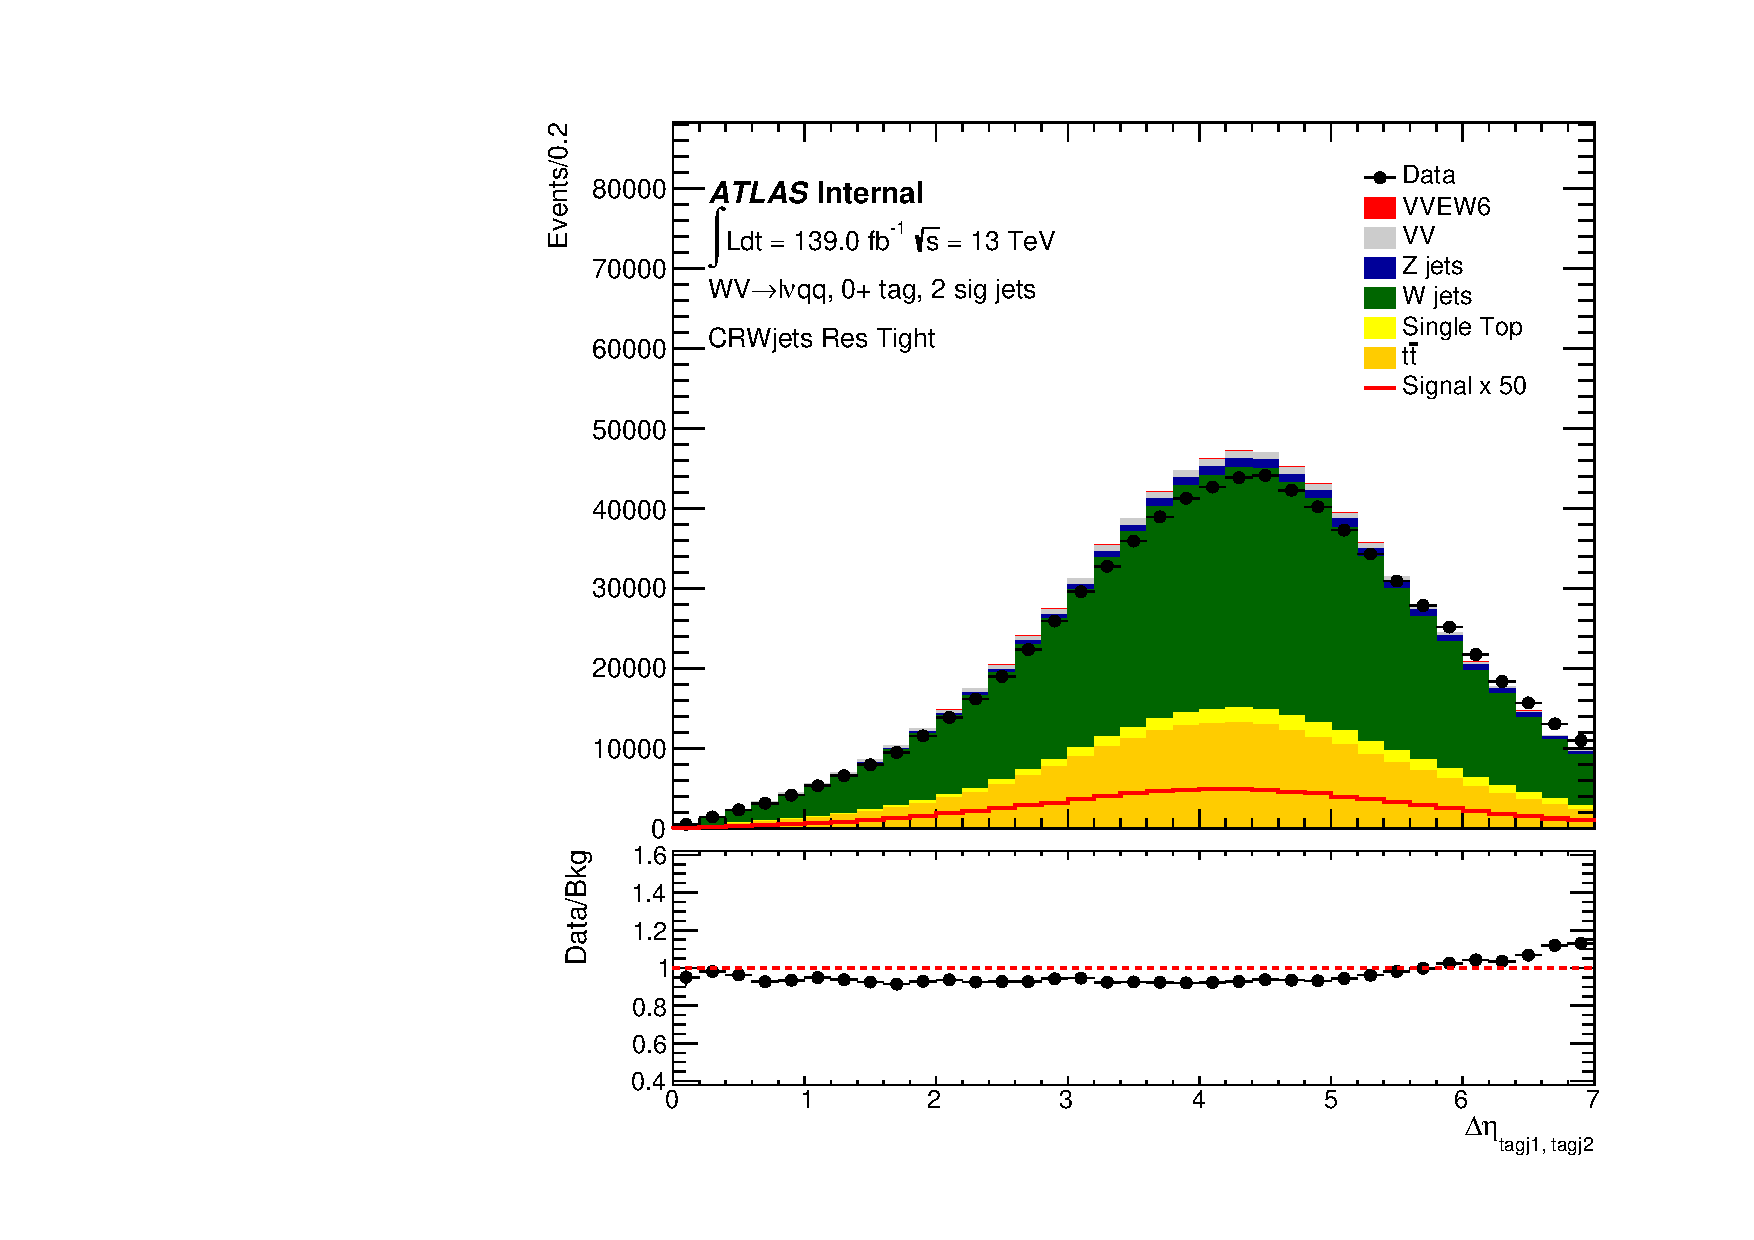
\includegraphics[width=0.3\textwidth]{figures/CRPlots/CRWjets_Res_Tight/stacked_plot_resolved_tagJdEta.pdf}}
    \subfloat[]{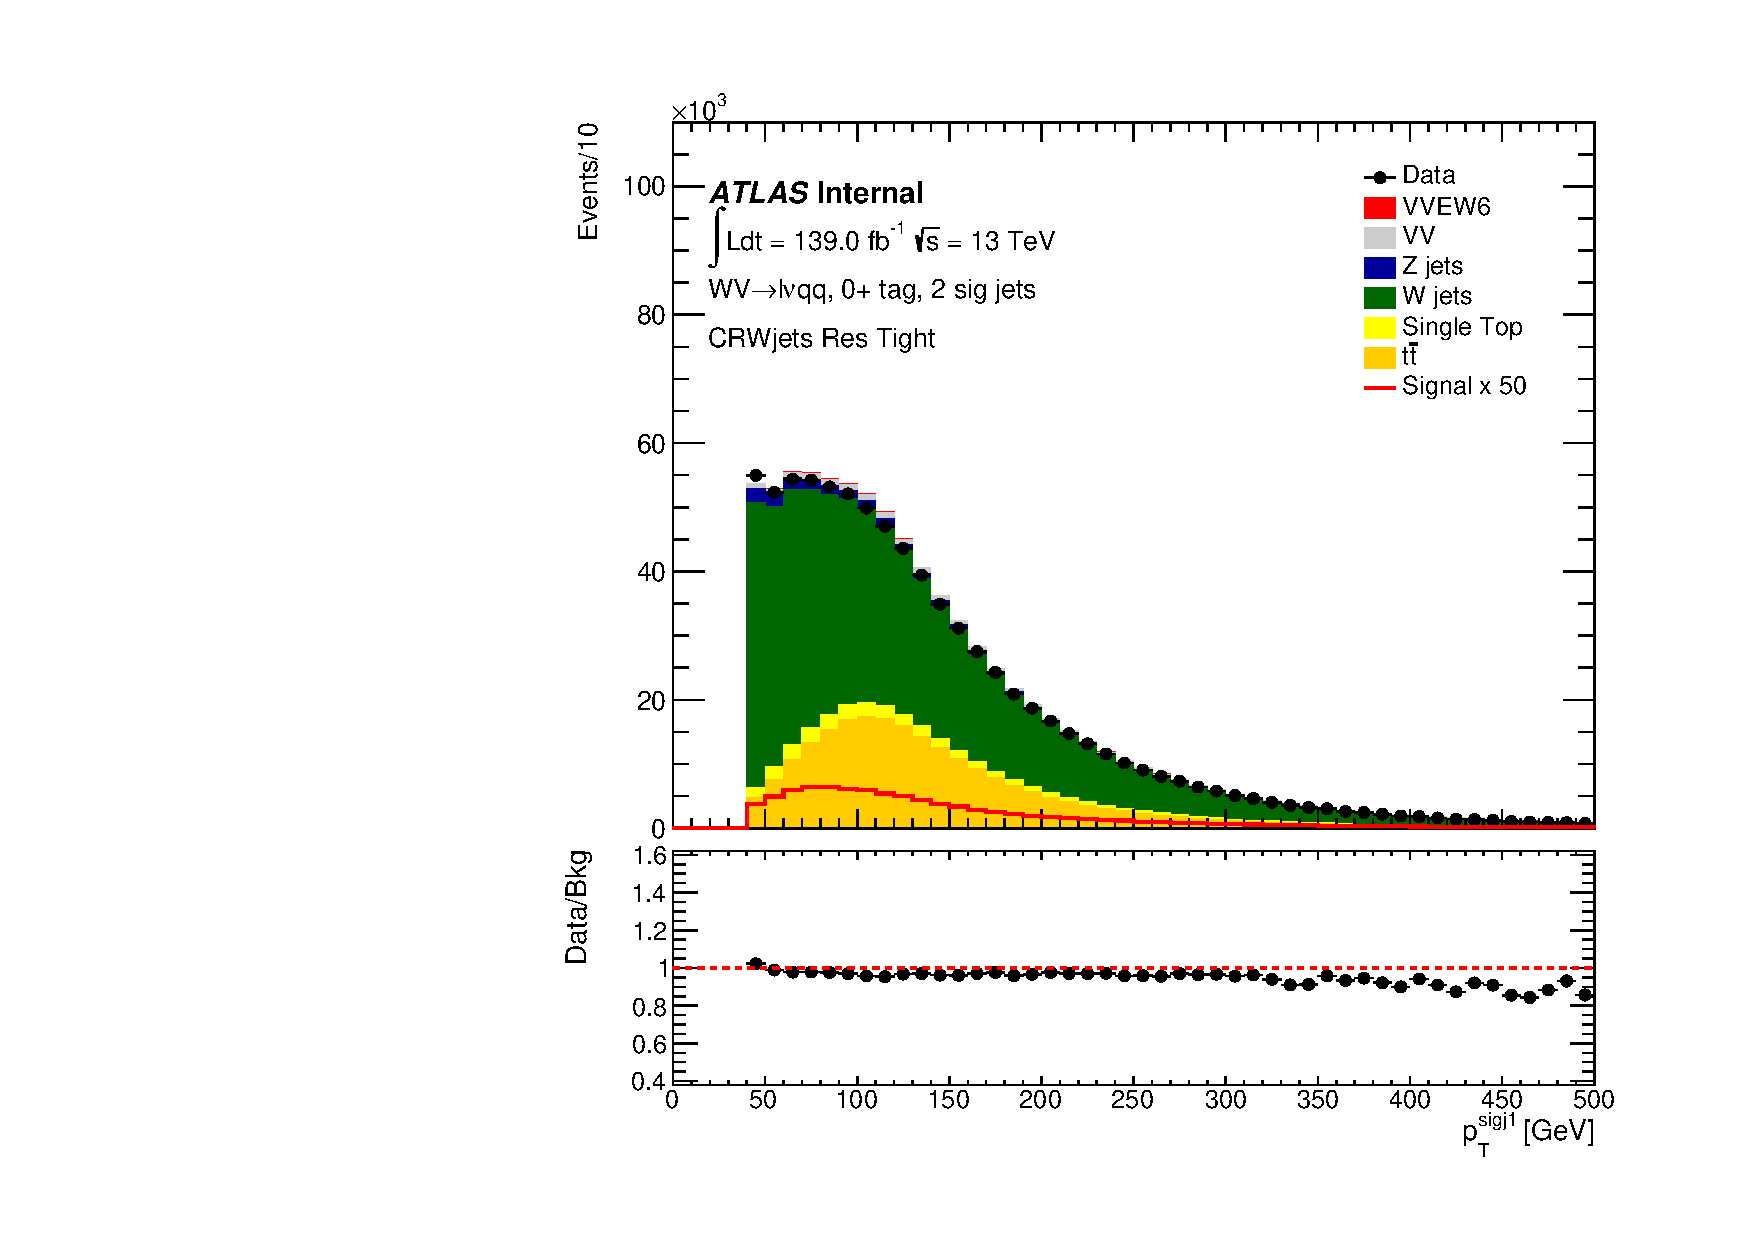
\includegraphics[width=0.3\textwidth]{figures/CRPlots/CRWjets_Res_Tight/stacked_plot_sigJ1_pt.pdf}}
    \subfloat[]{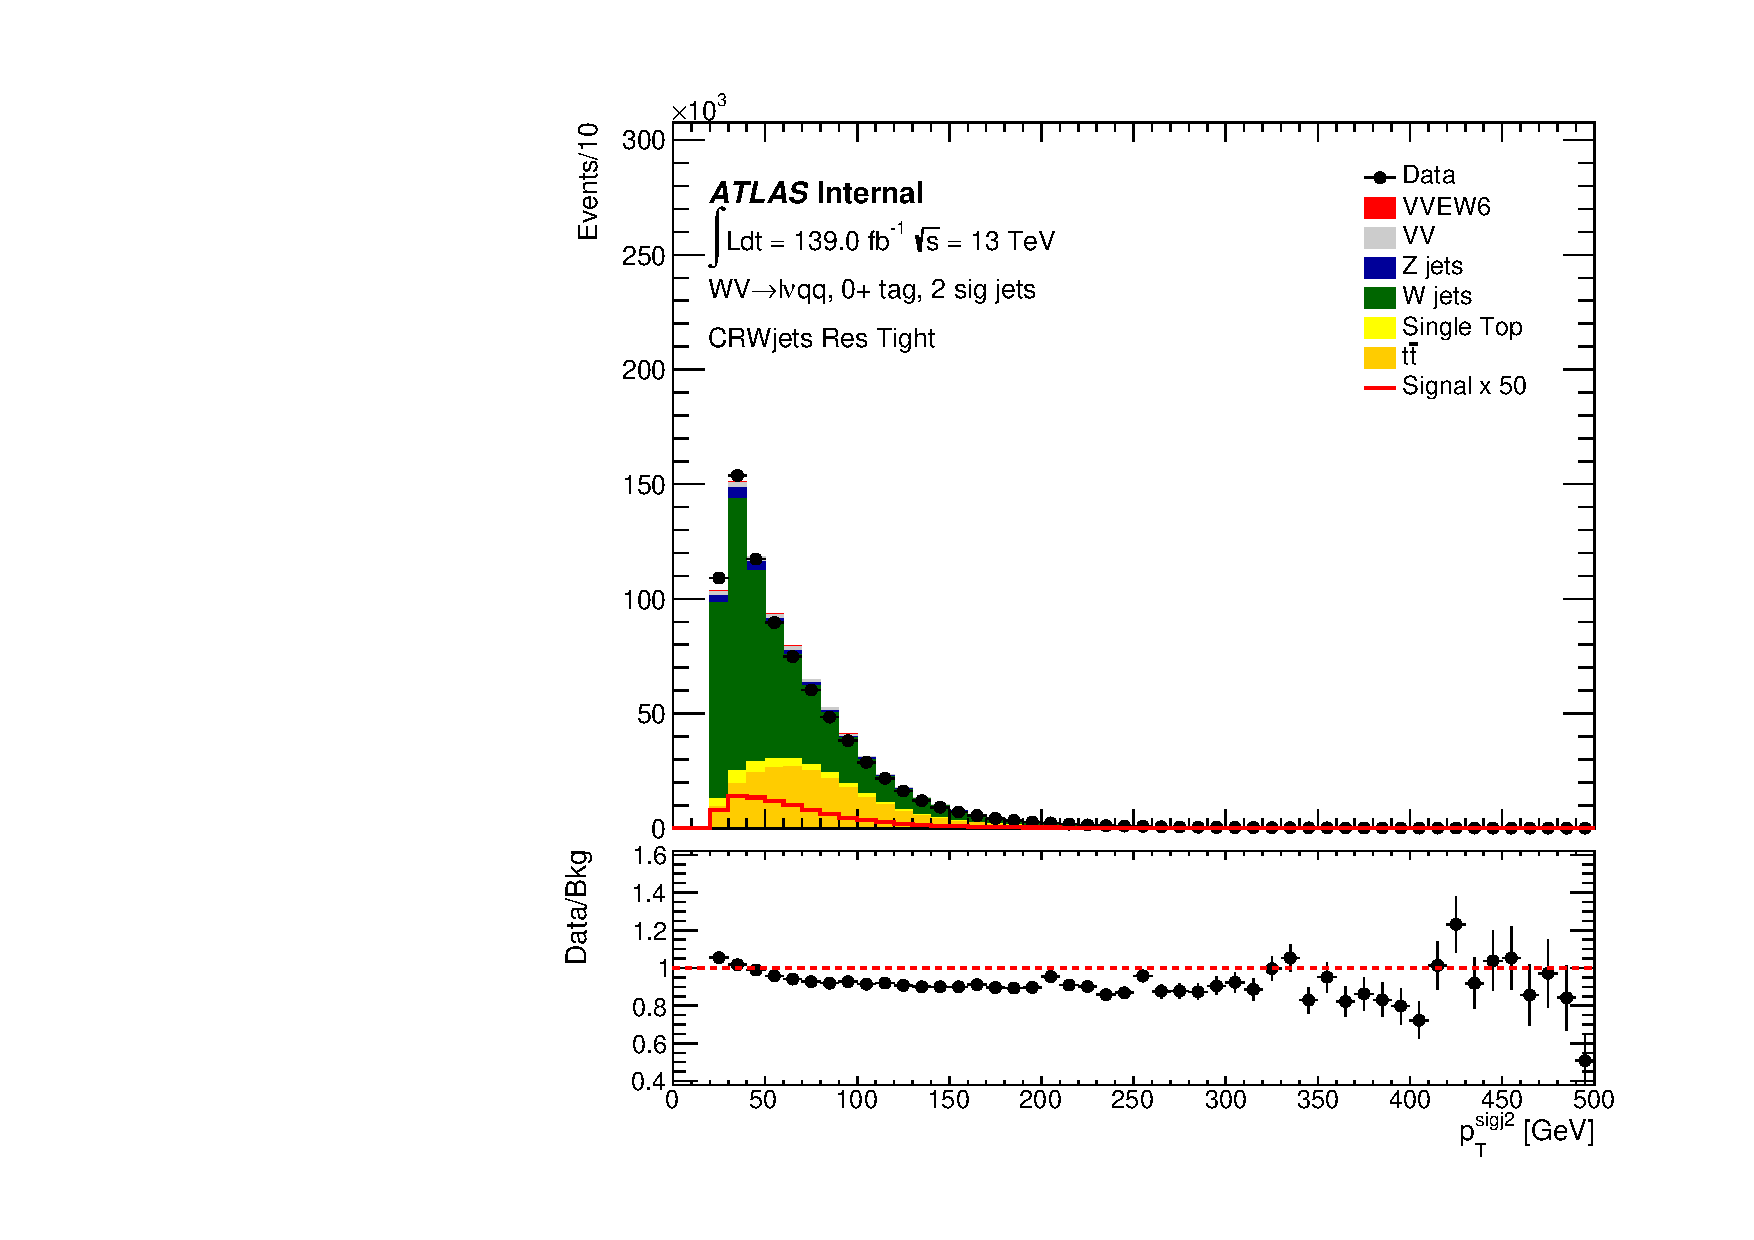
\includegraphics[width=0.3\textwidth]{figures/CRPlots/CRWjets_Res_Tight/stacked_plot_sigJ2_pt.pdf}} \\
    \subfloat[]{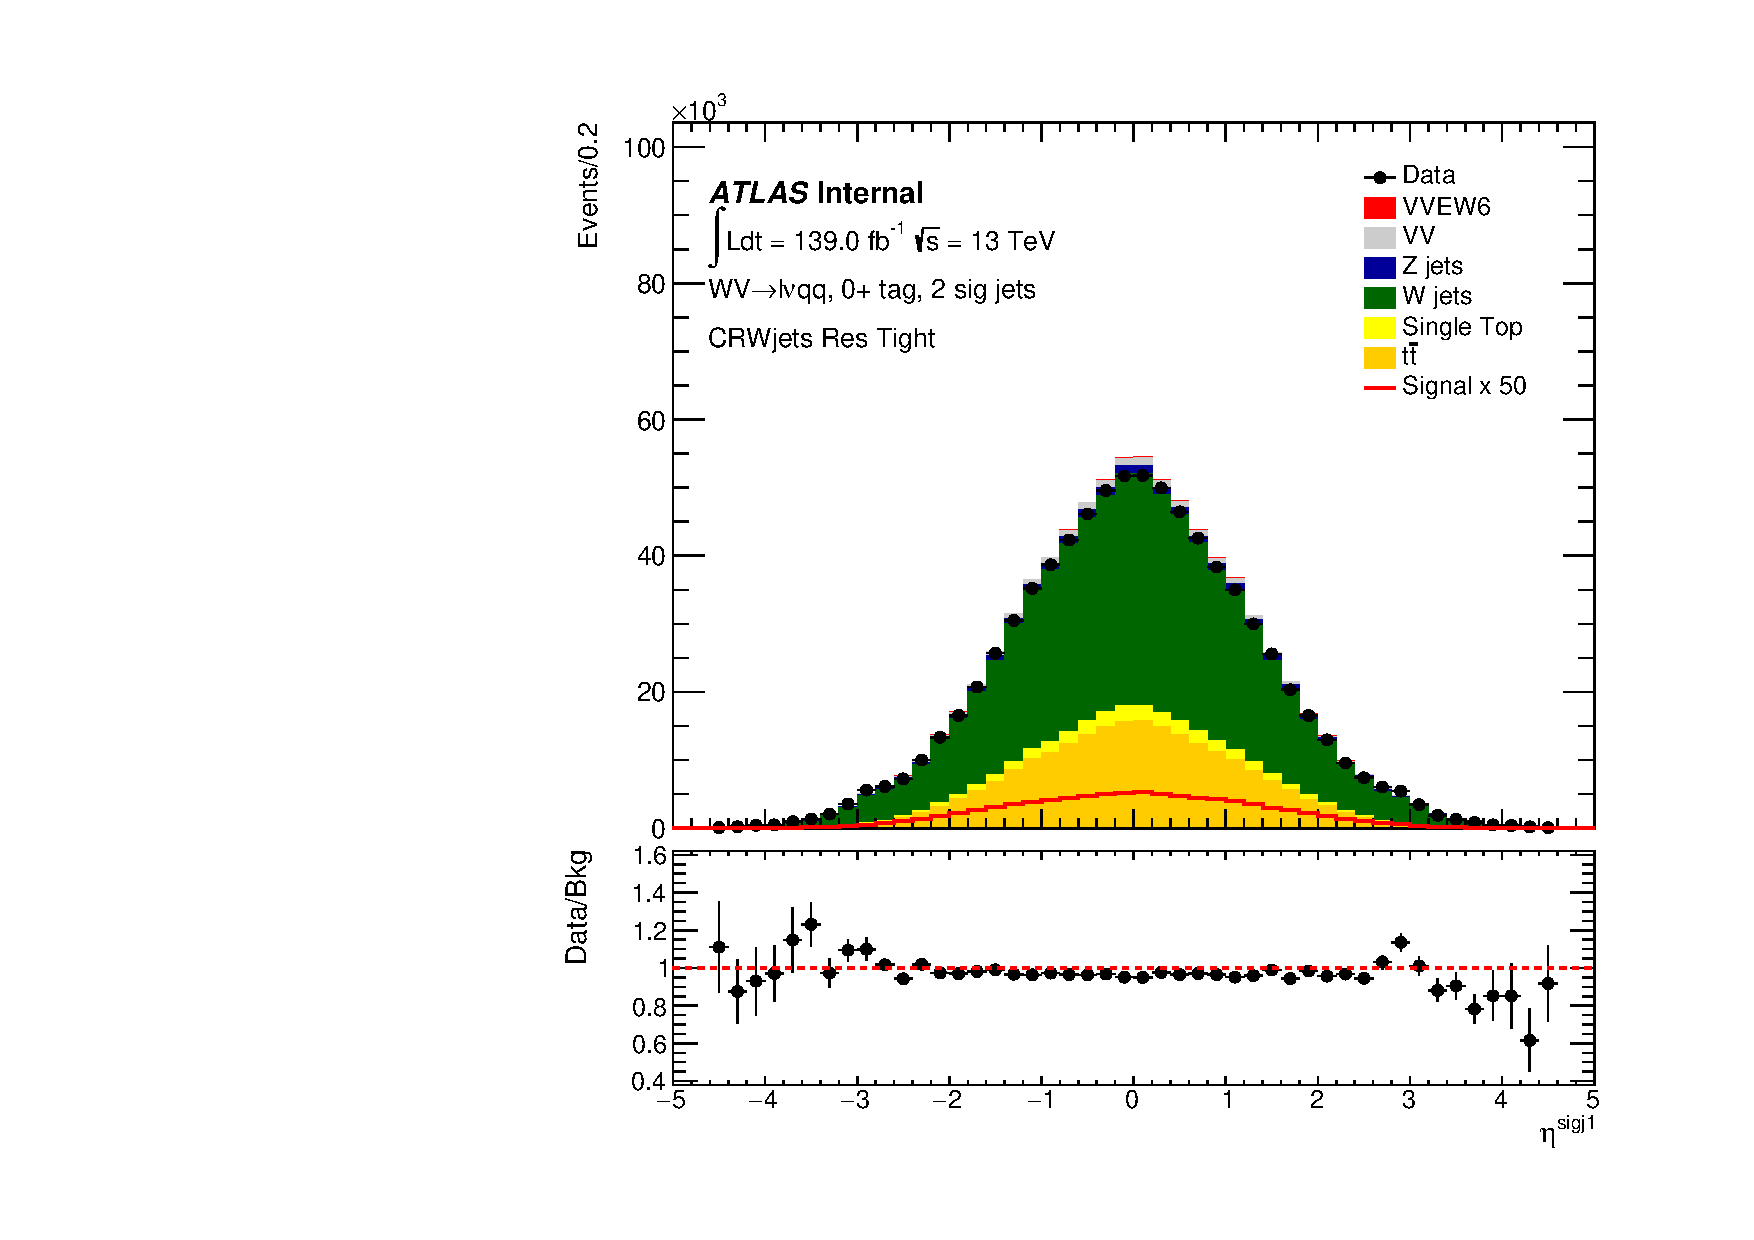
\includegraphics[width=0.3\textwidth]{figures/CRPlots/CRWjets_Res_Tight/stacked_plot_sigJ1_eta.pdf}}
    \subfloat[]{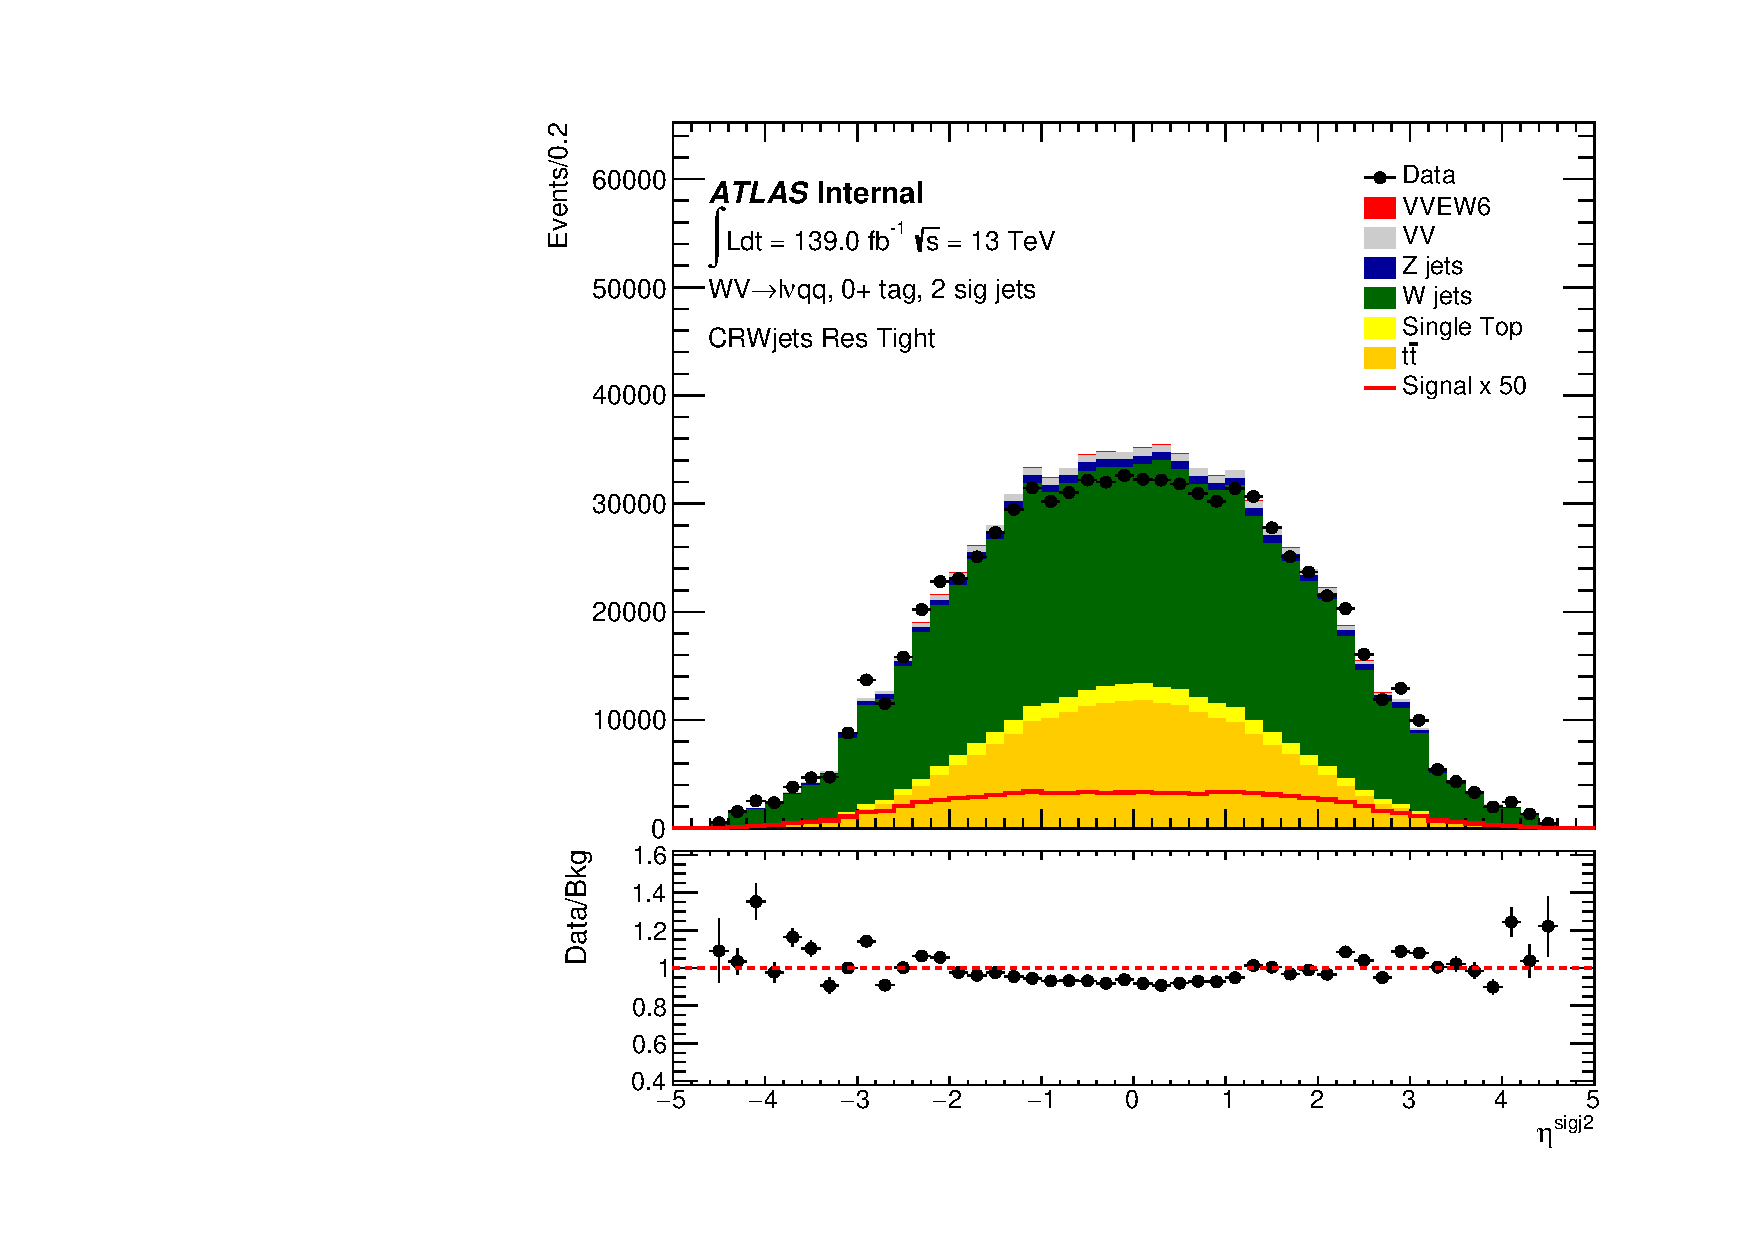
\includegraphics[width=0.3\textwidth]{figures/CRPlots/CRWjets_Res_Tight/stacked_plot_sigJ2_eta.pdf}} \\
    \subfloat[]{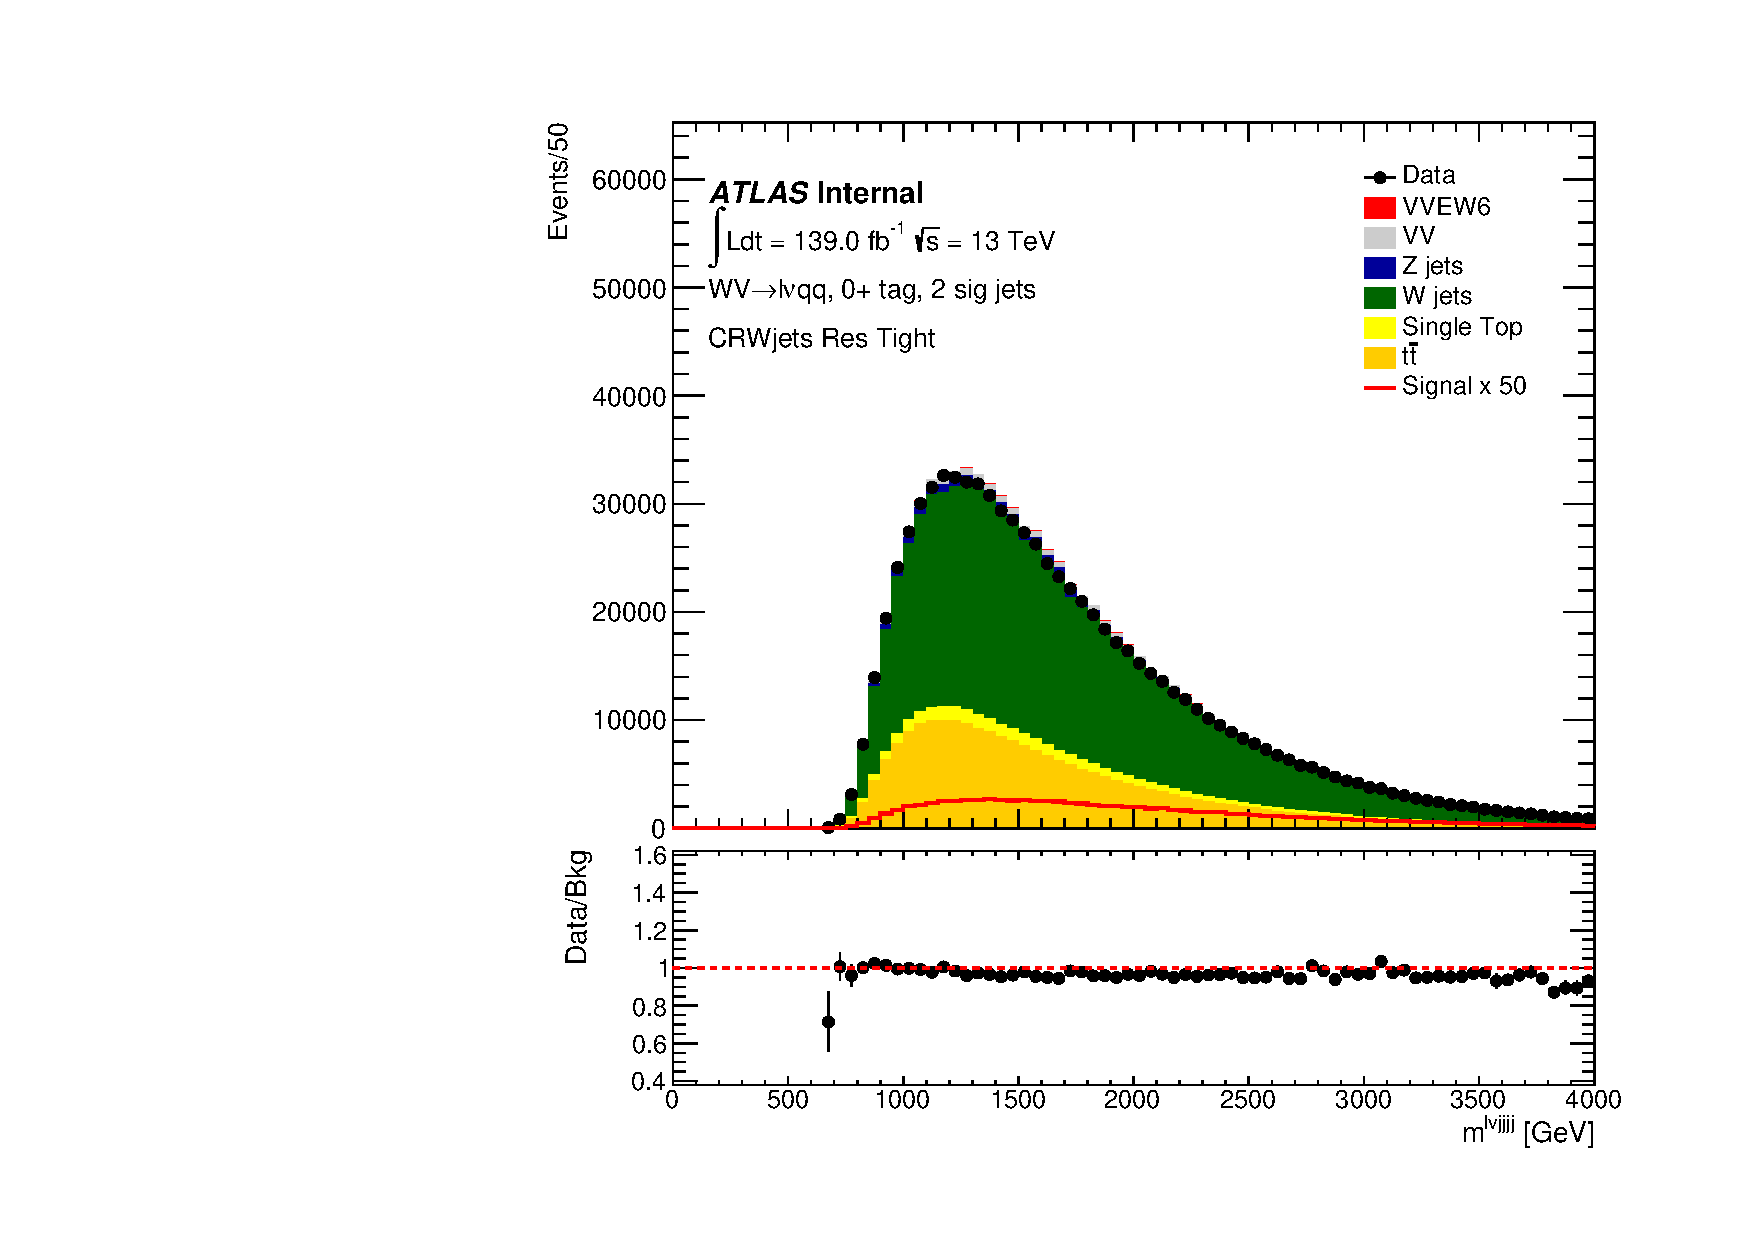
\includegraphics[width=0.3\textwidth]{figures/CRPlots/CRWjets_Res_Tight/stacked_plot_lvjjjjmass.pdf}}
    \subfloat[]{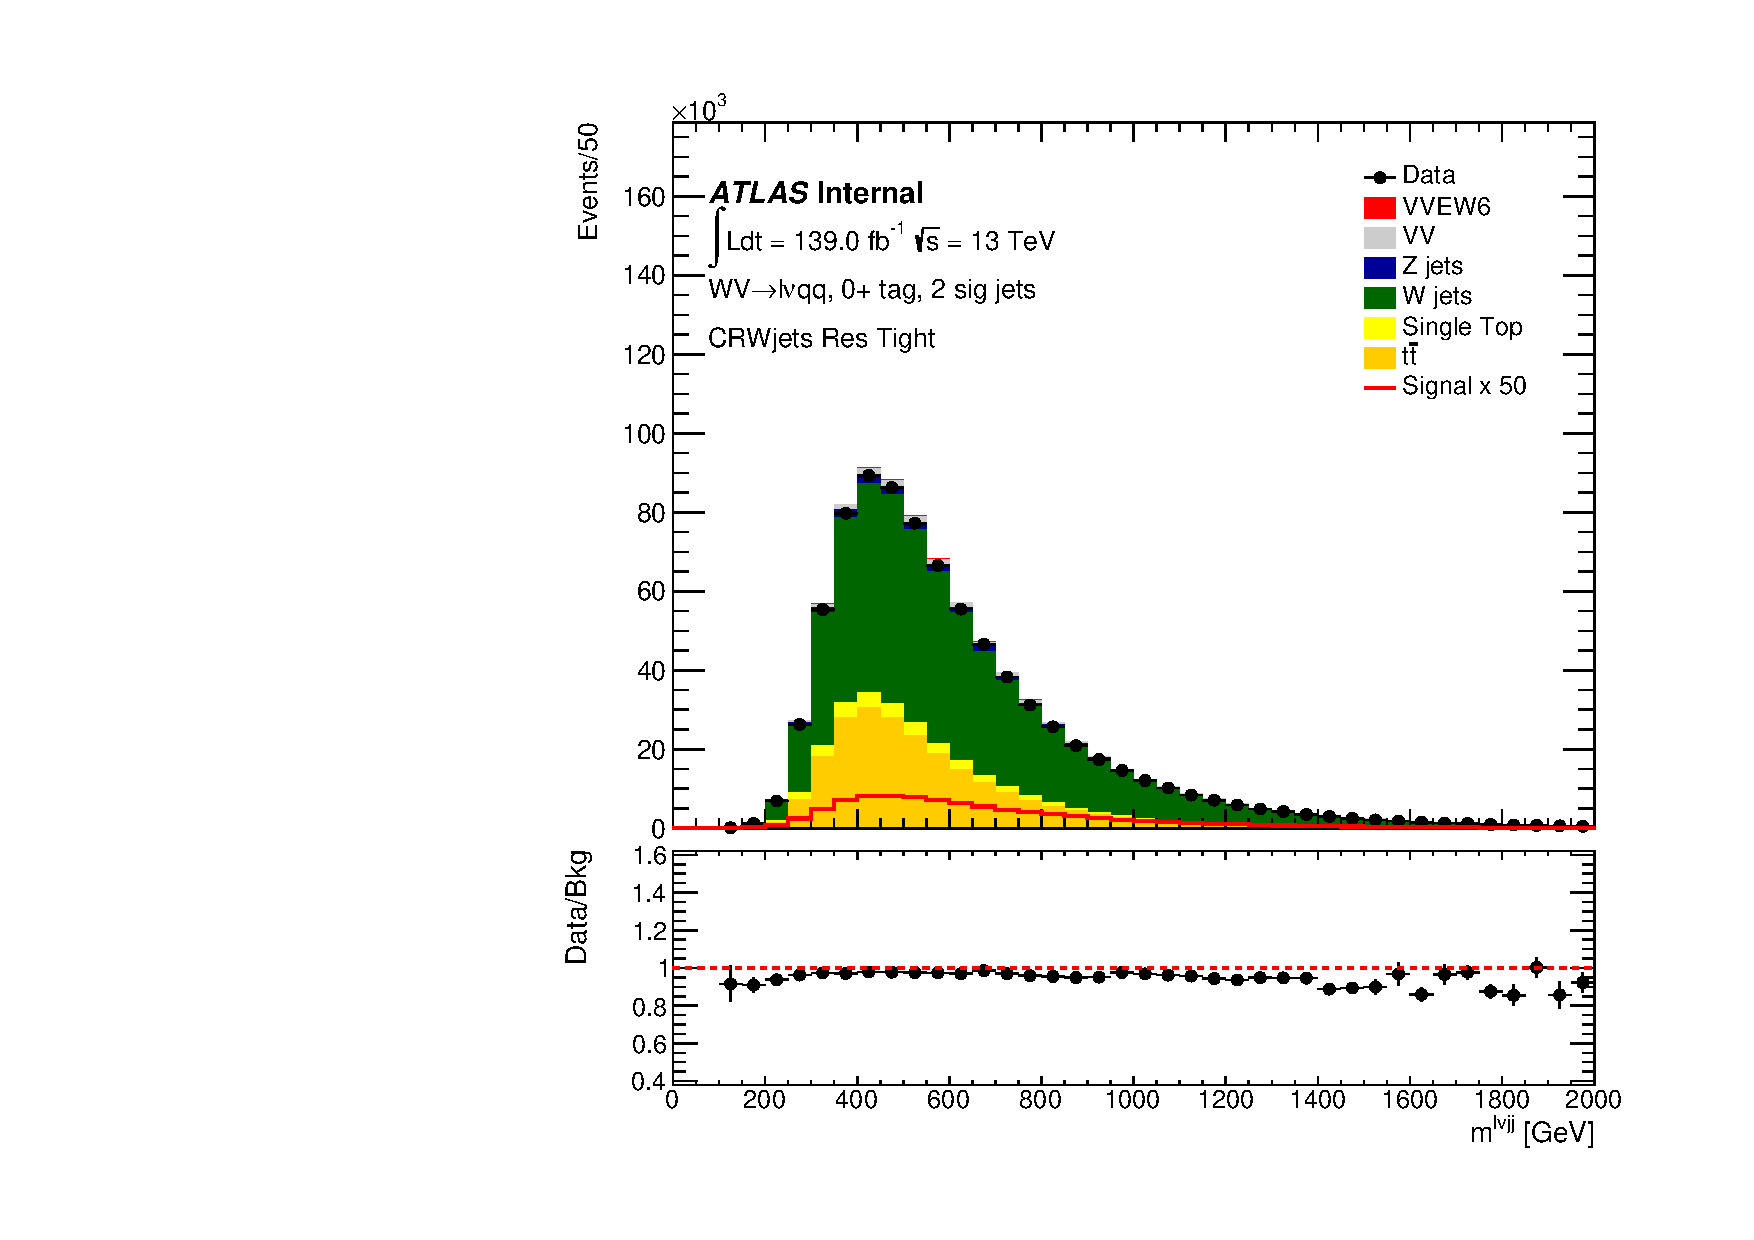
\includegraphics[width=0.3\textwidth]{figures/CRPlots/CRWjets_Res_Tight/stacked_plot_lvjjmass.pdf}}
    \subfloat[]{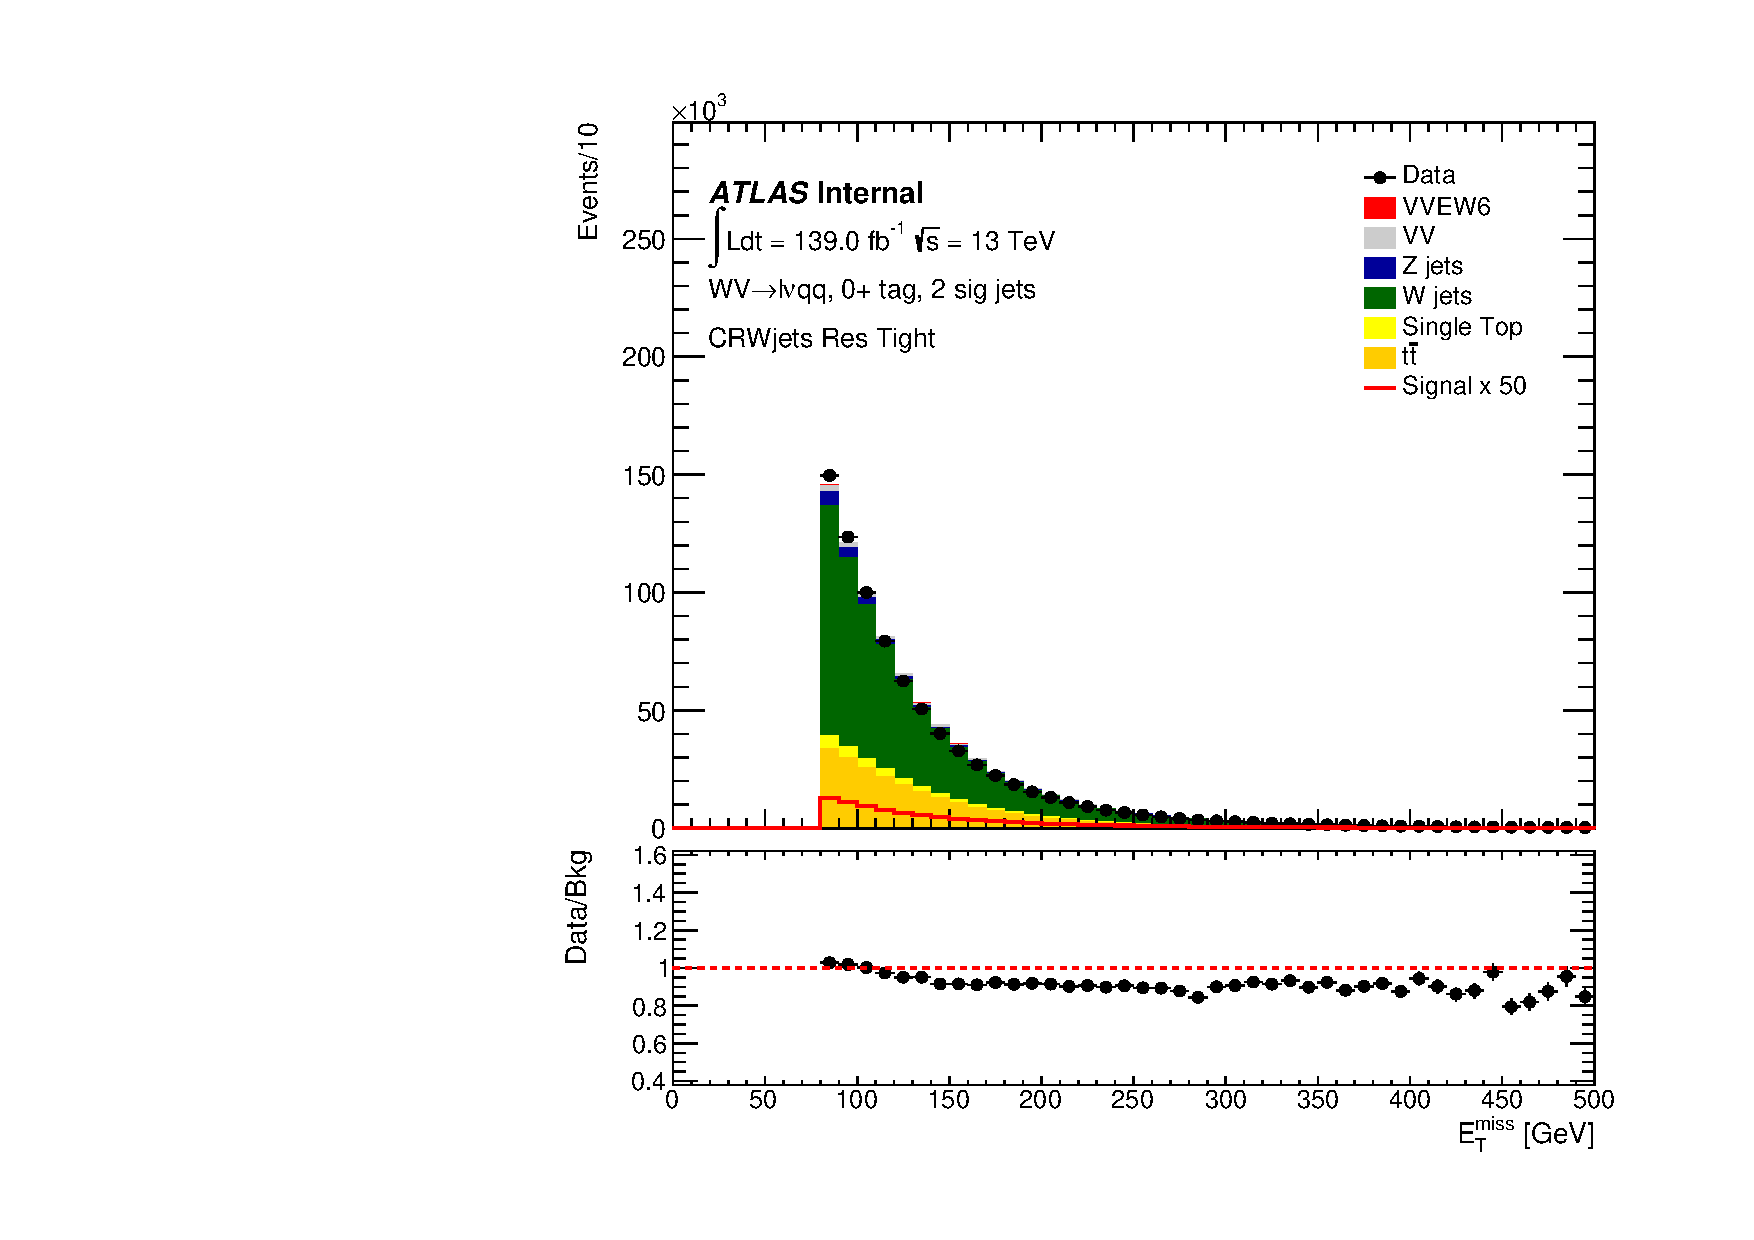
\includegraphics[width=0.3\textwidth]{figures/CRPlots/CRWjets_Res_Tight/stacked_plot_met.pdf}}  %%\\
%%    \subfloat[]{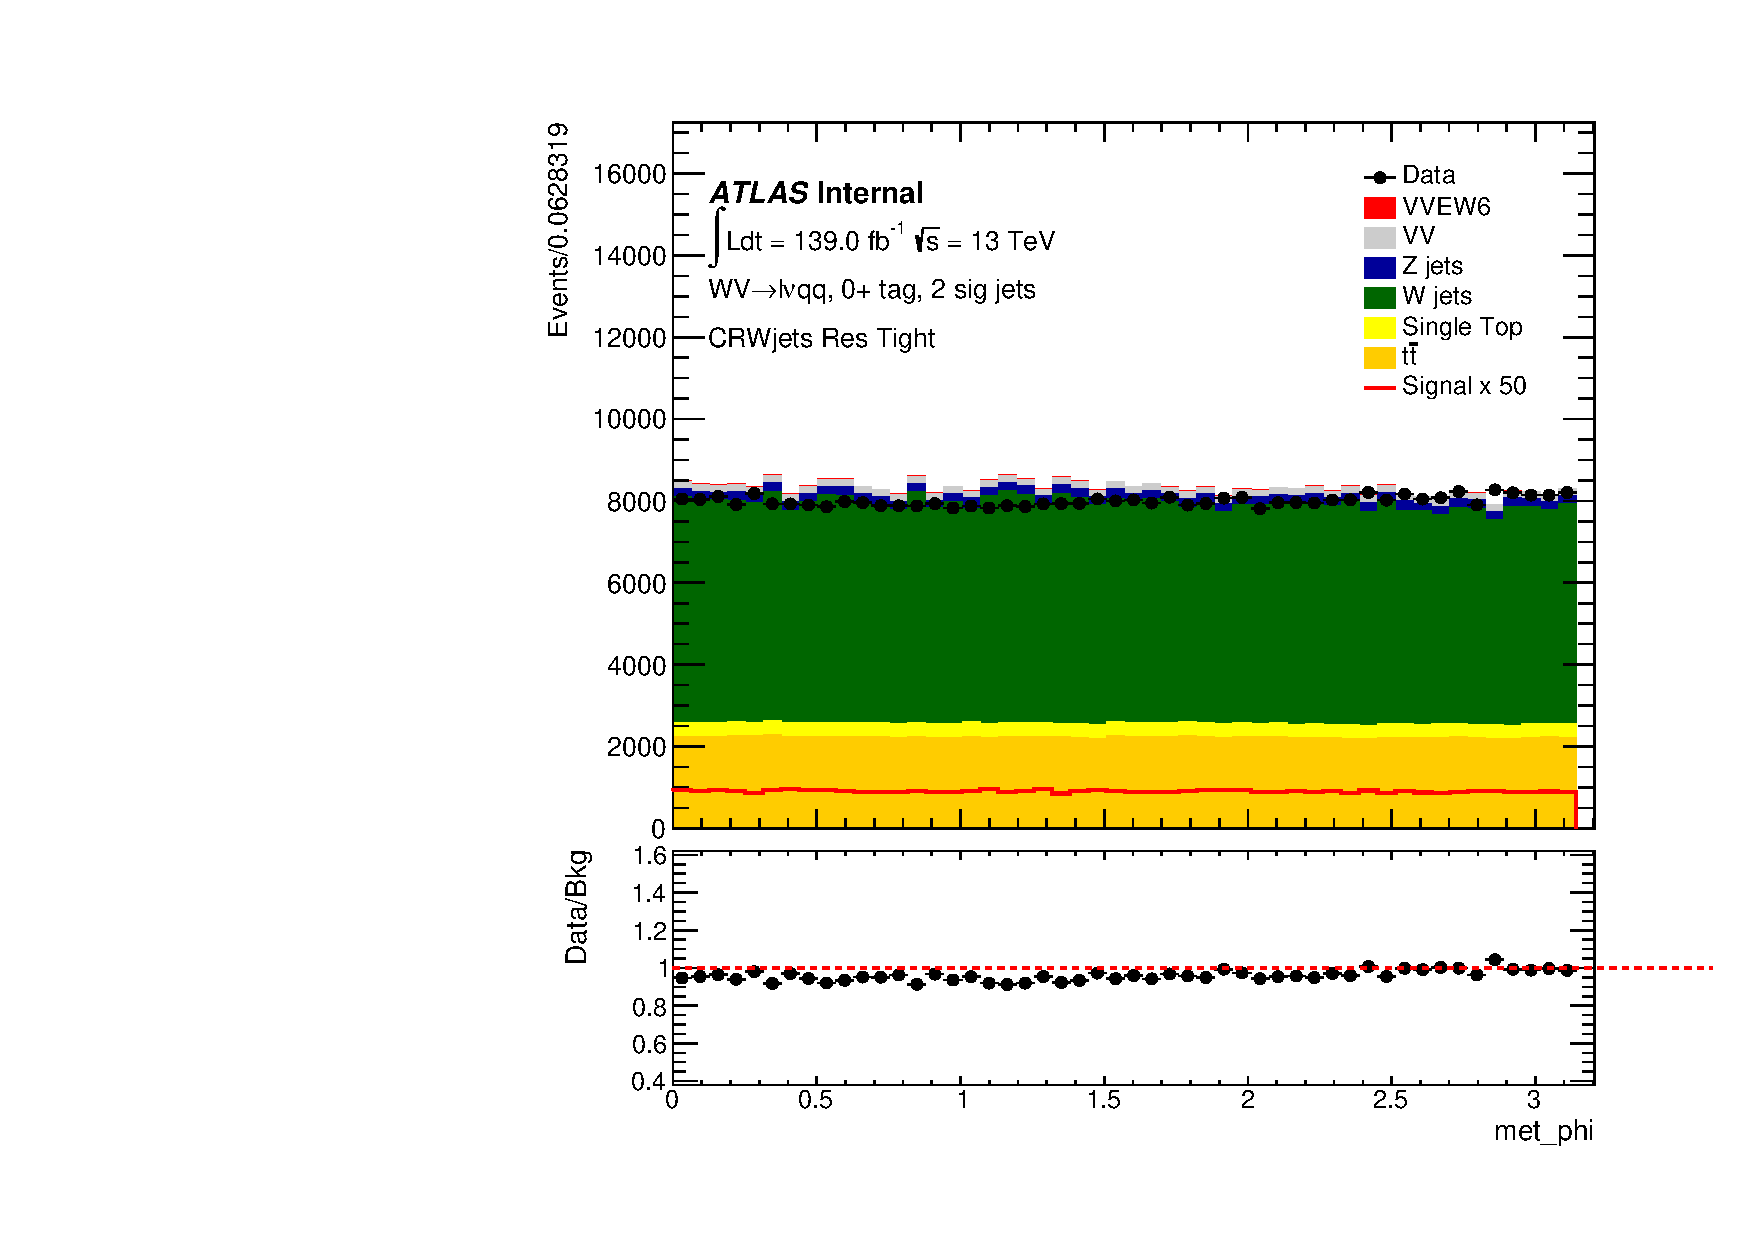
\includegraphics[width=0.3\textwidth]{figures/CRPlots/CRWjets_Res_Tight/stacked_plot_met_phi.pdf}}
%%    \subfloat[]{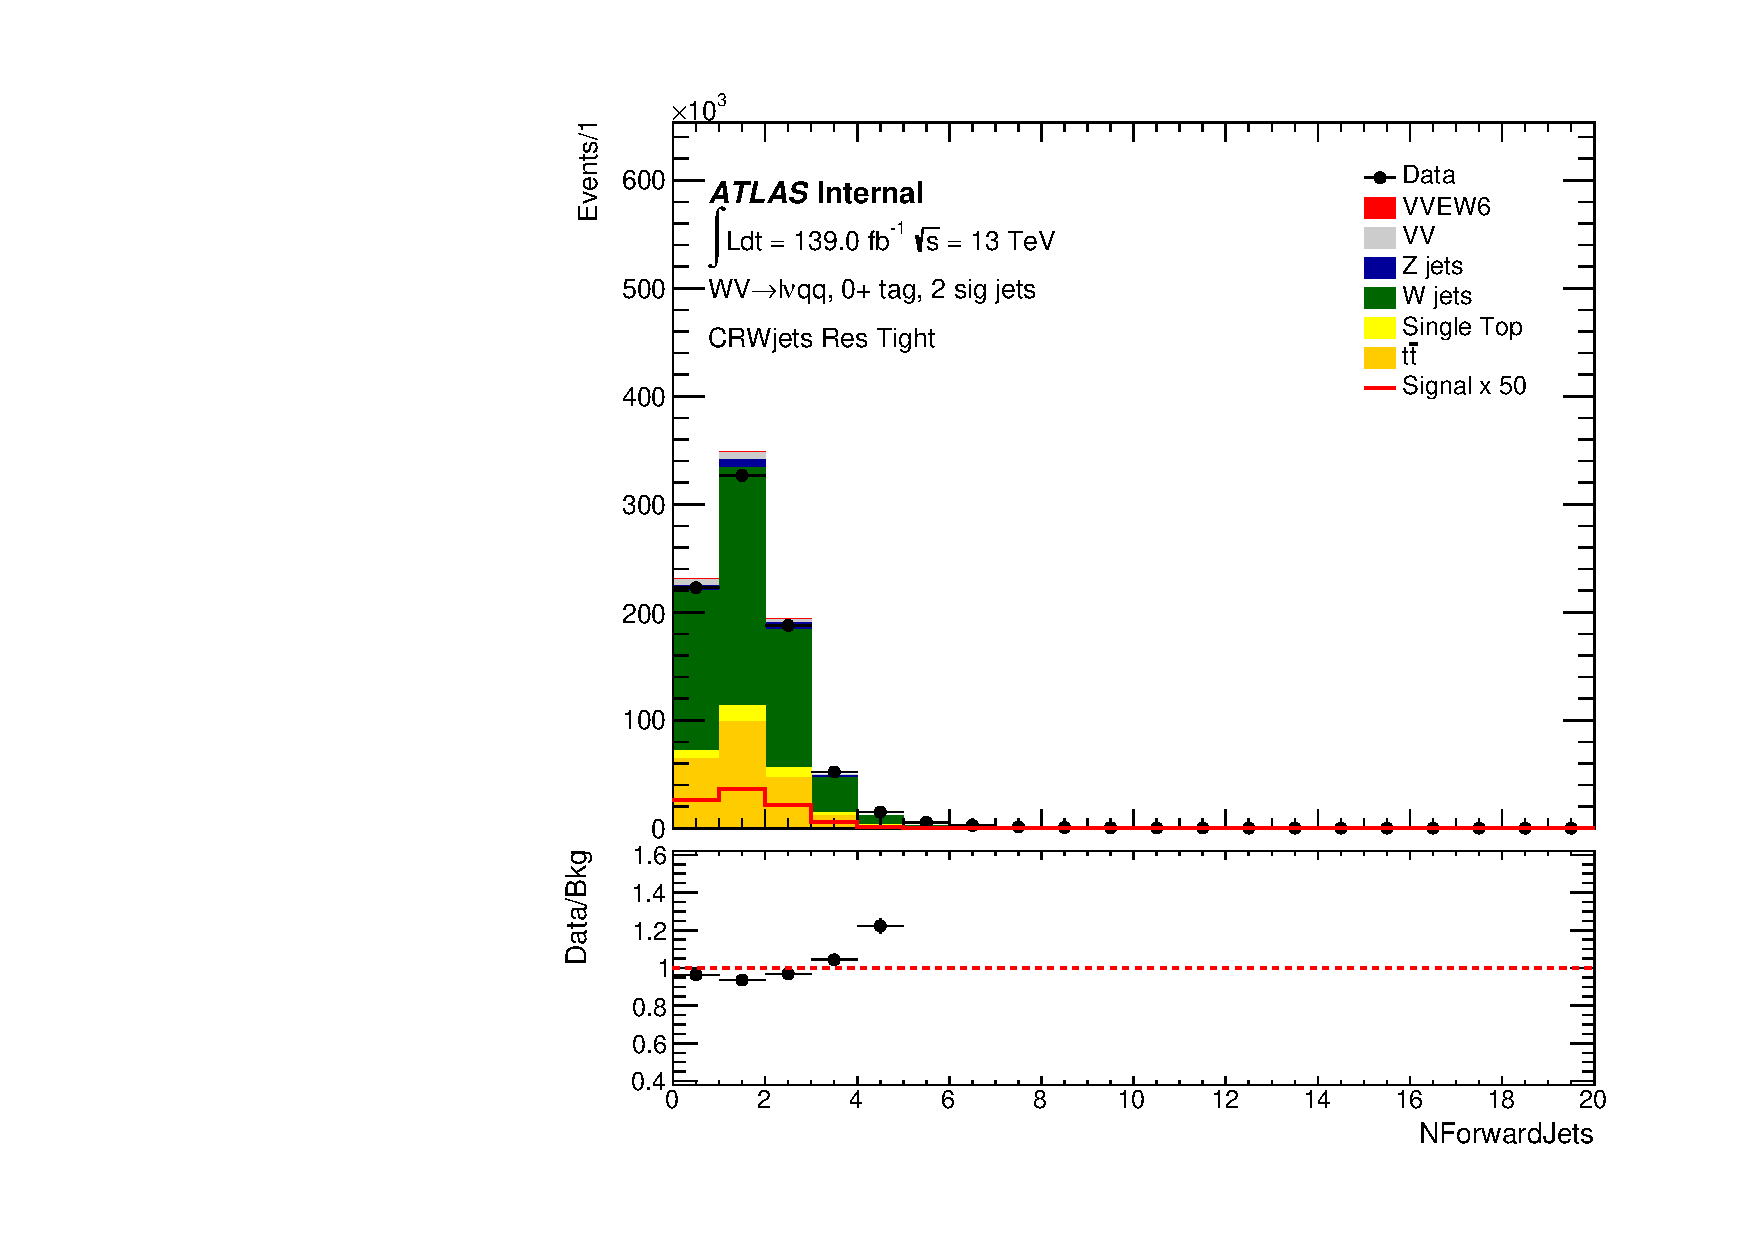
\includegraphics[width=0.3\textwidth]{figures/CRPlots/CRWjets_Res_Tight/stacked_plot_NForwardJets.pdf}}
    \caption{Data-MC checks for the resolved tight \Wjets control region in the \olep channel.}
    \label{fig:CRWjetResTightPlots1Lep2}
\end{figure}

\begin{figure}[ht]
    \centering
    \subfloat[]{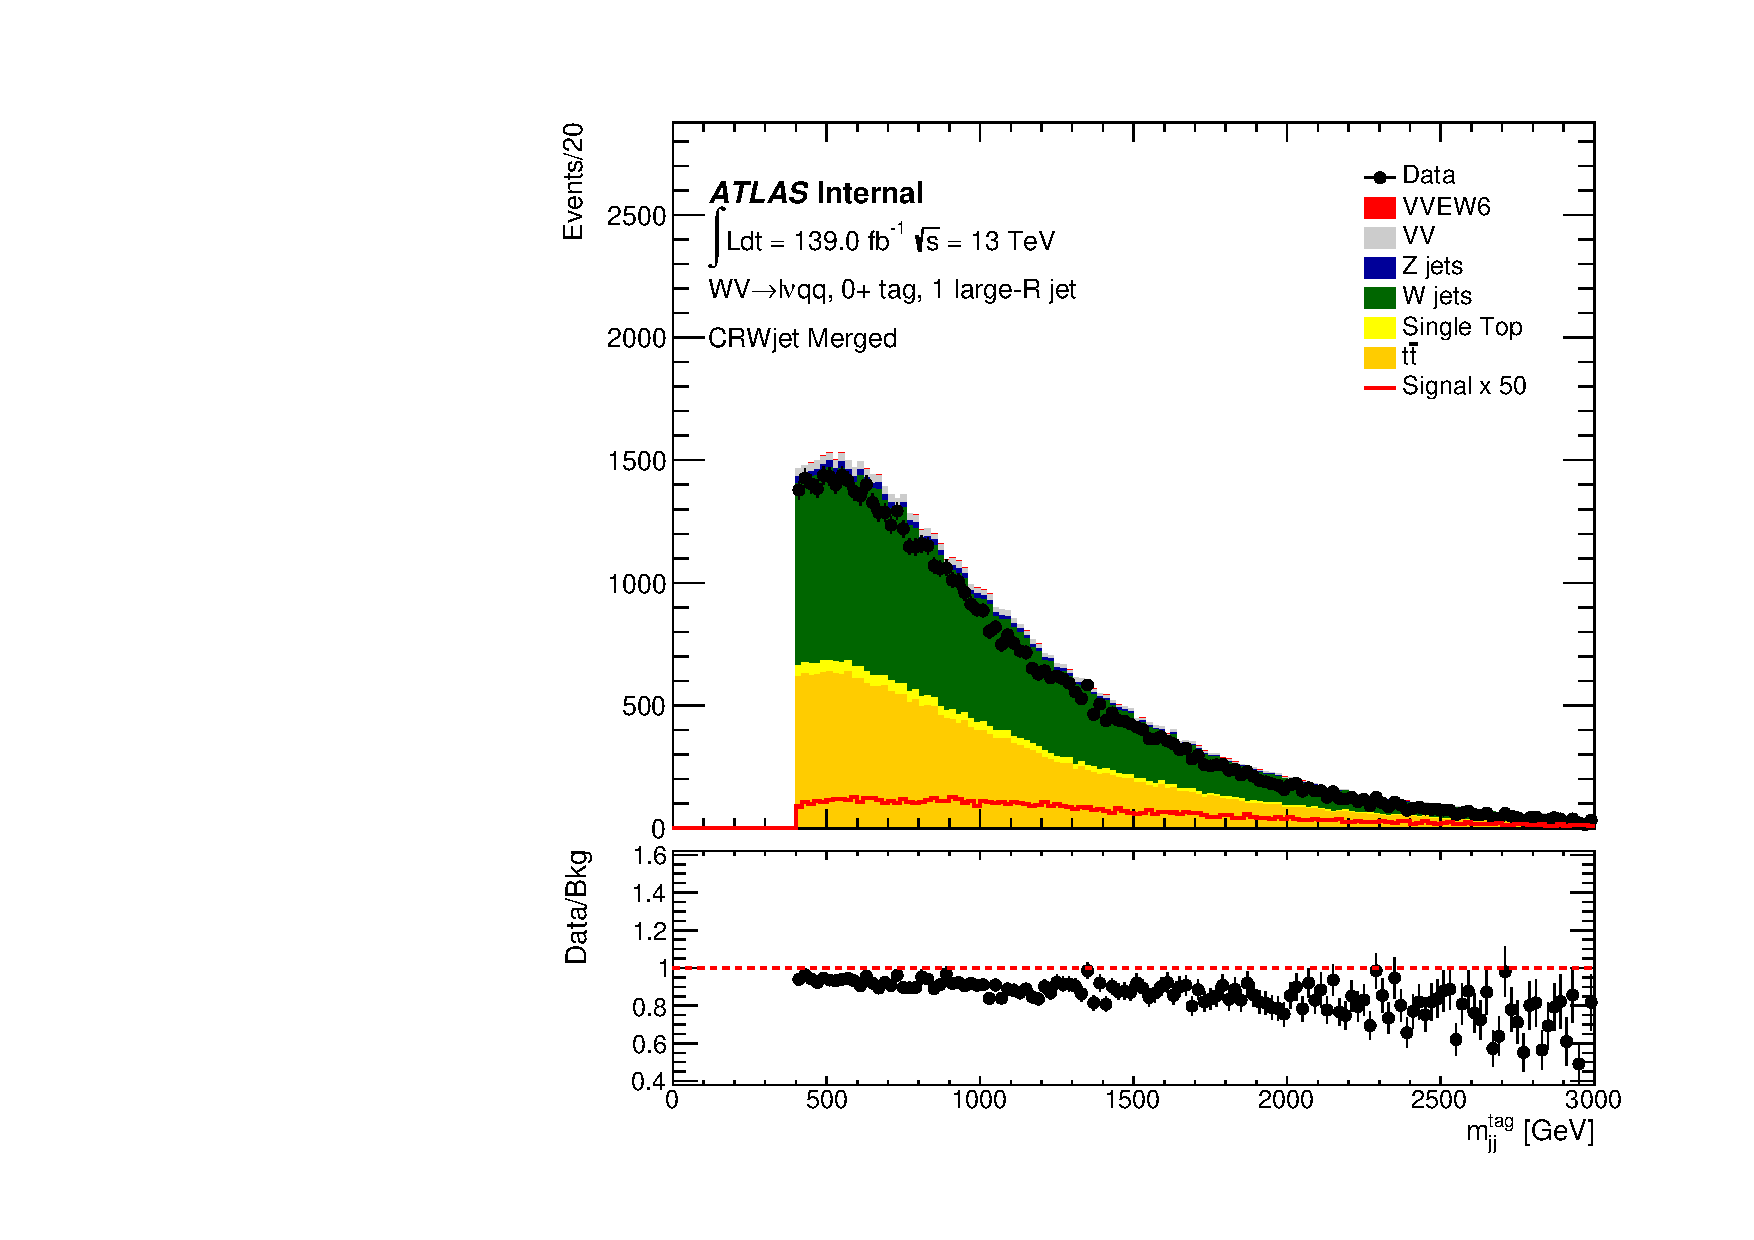
\includegraphics[width=0.3\textwidth]{figures/CRPlots/CRWjets100/stacked_plot_merged_tagMjj.pdf}}
    \subfloat[]{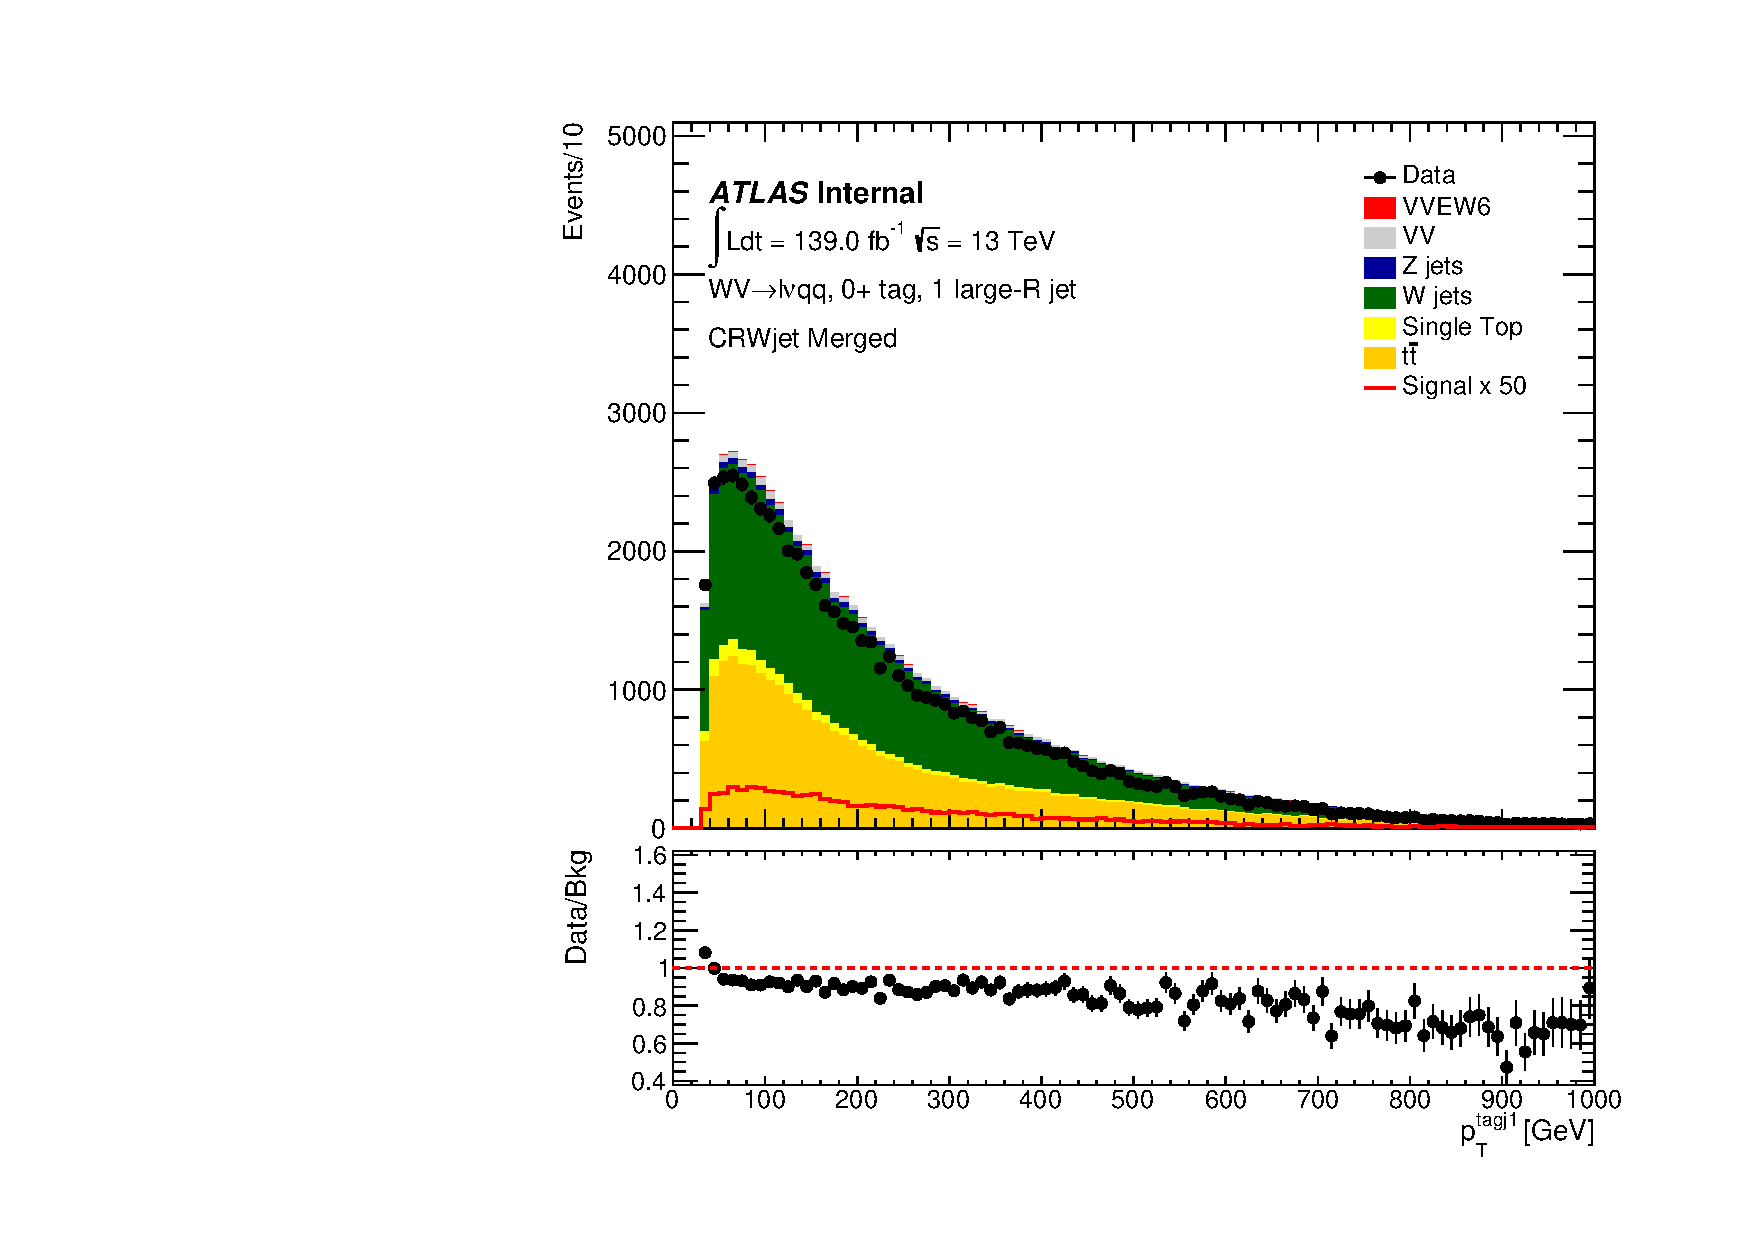
\includegraphics[width=0.3\textwidth]{figures/CRPlots/CRWjets100/stacked_plot_merged_tagJ1_pt.pdf}}
    \subfloat[]{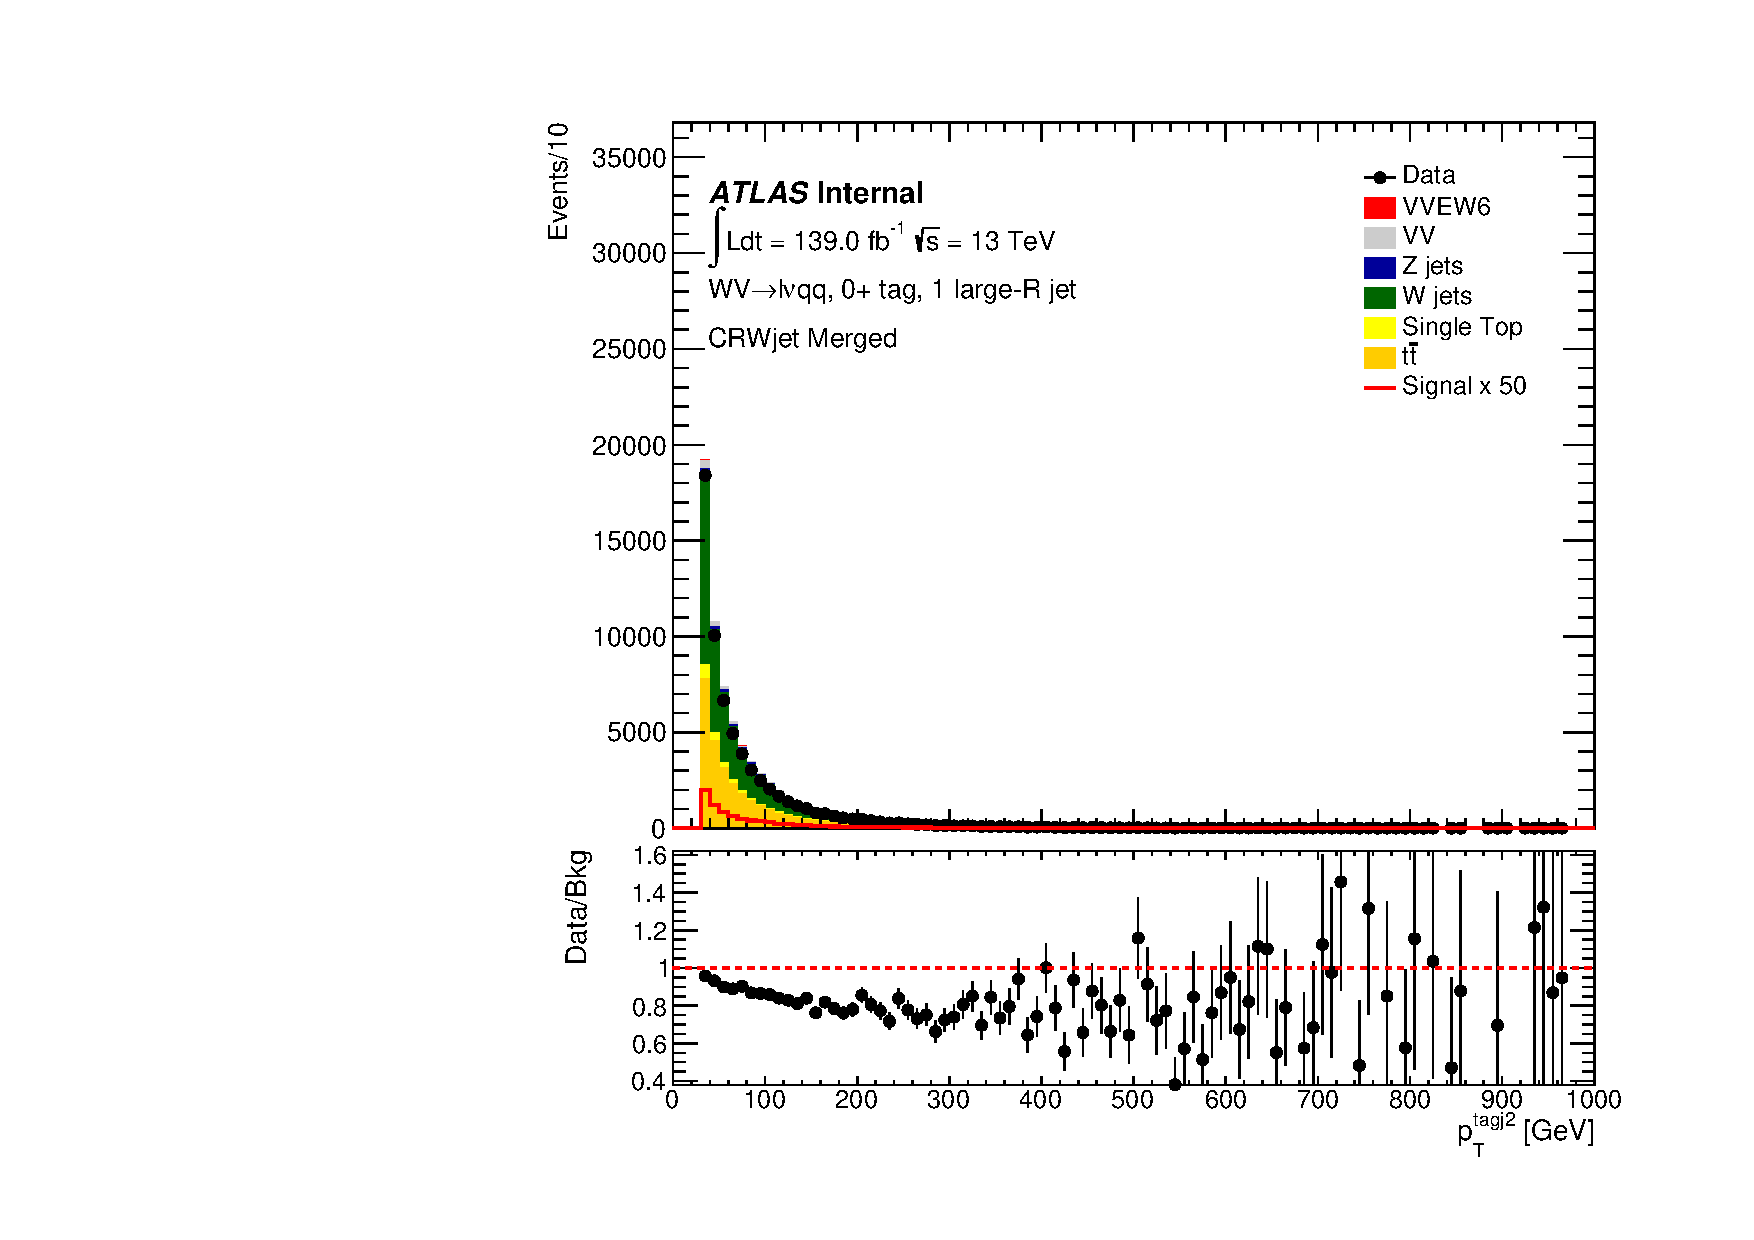
\includegraphics[width=0.3\textwidth]{figures/CRPlots/CRWjets100/stacked_plot_merged_tagJ2_pt.pdf}} \\
    \subfloat[]{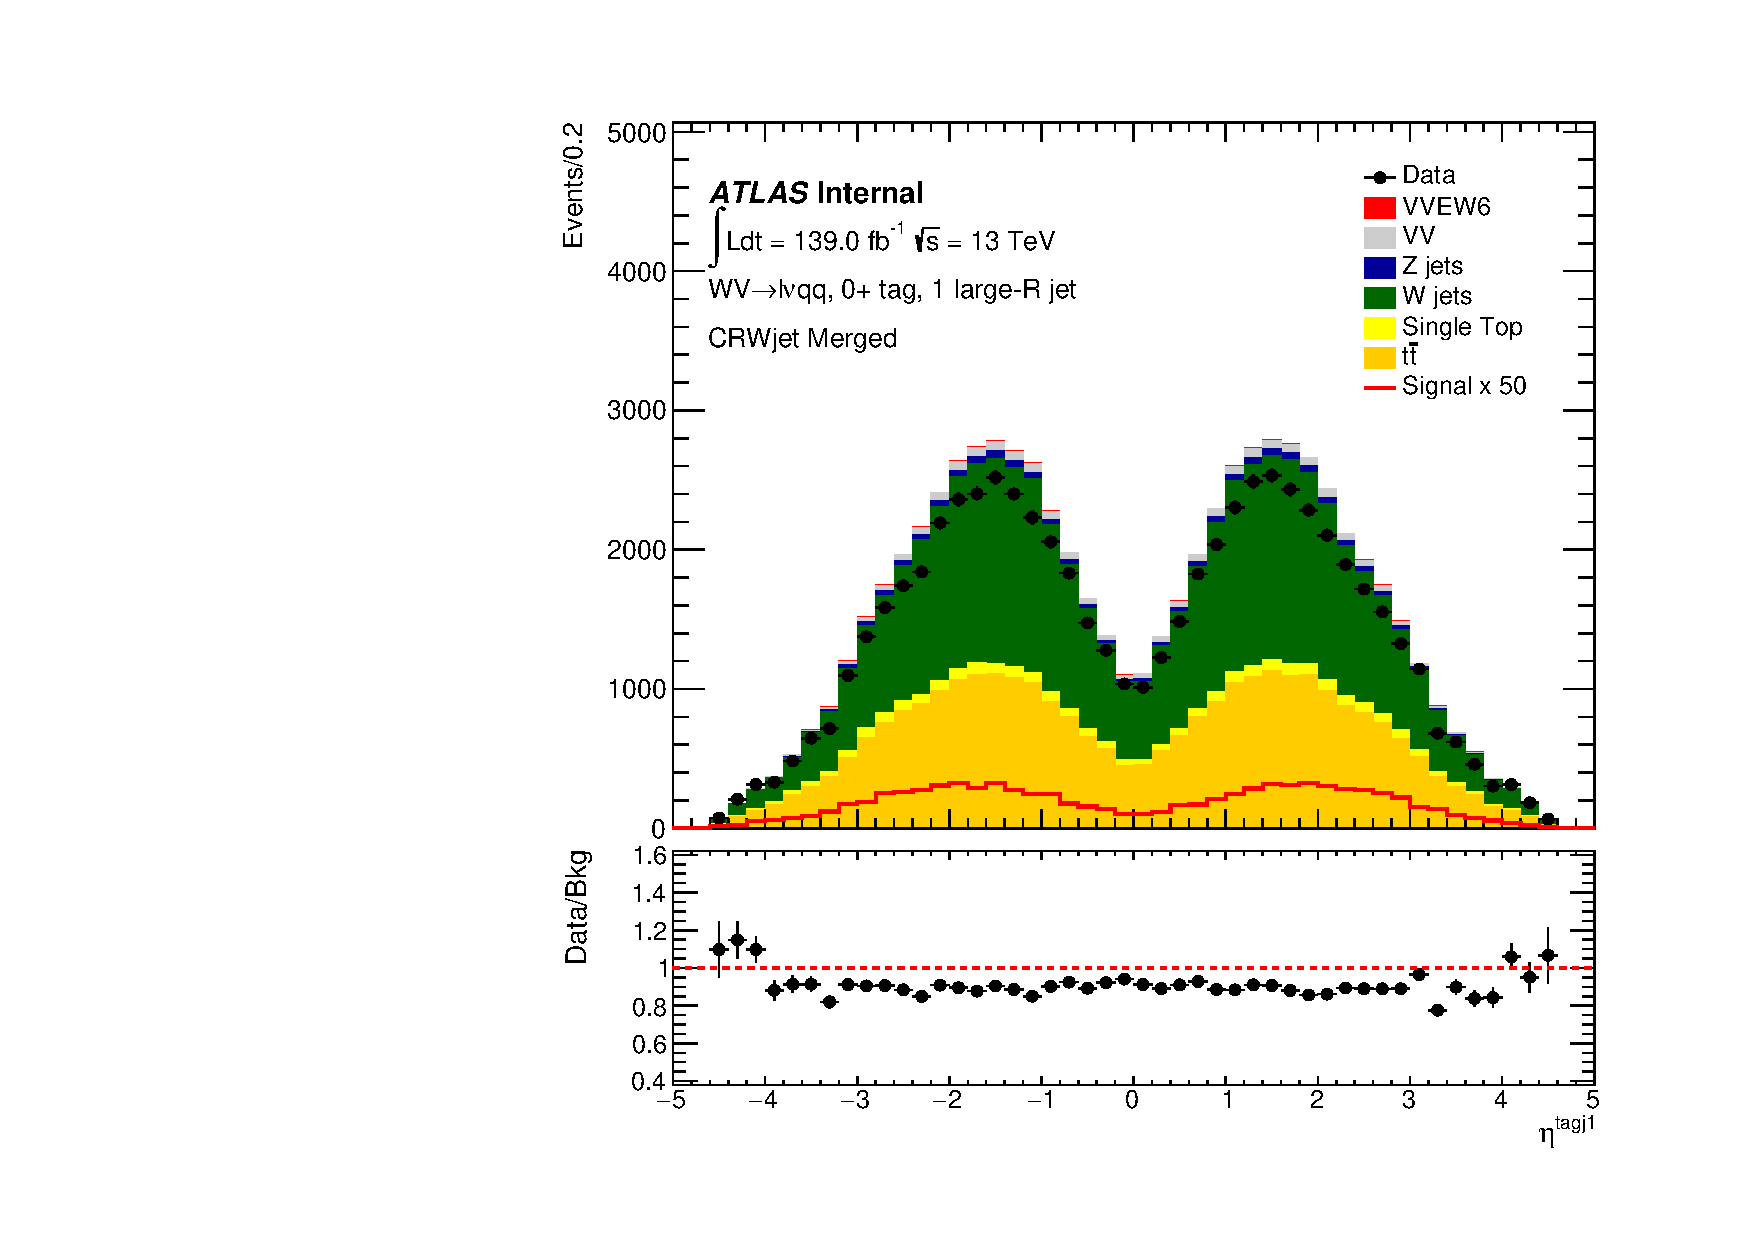
\includegraphics[width=0.3\textwidth]{figures/CRPlots/CRWjets100/stacked_plot_merged_tagJ1_eta.pdf}}
    \subfloat[]{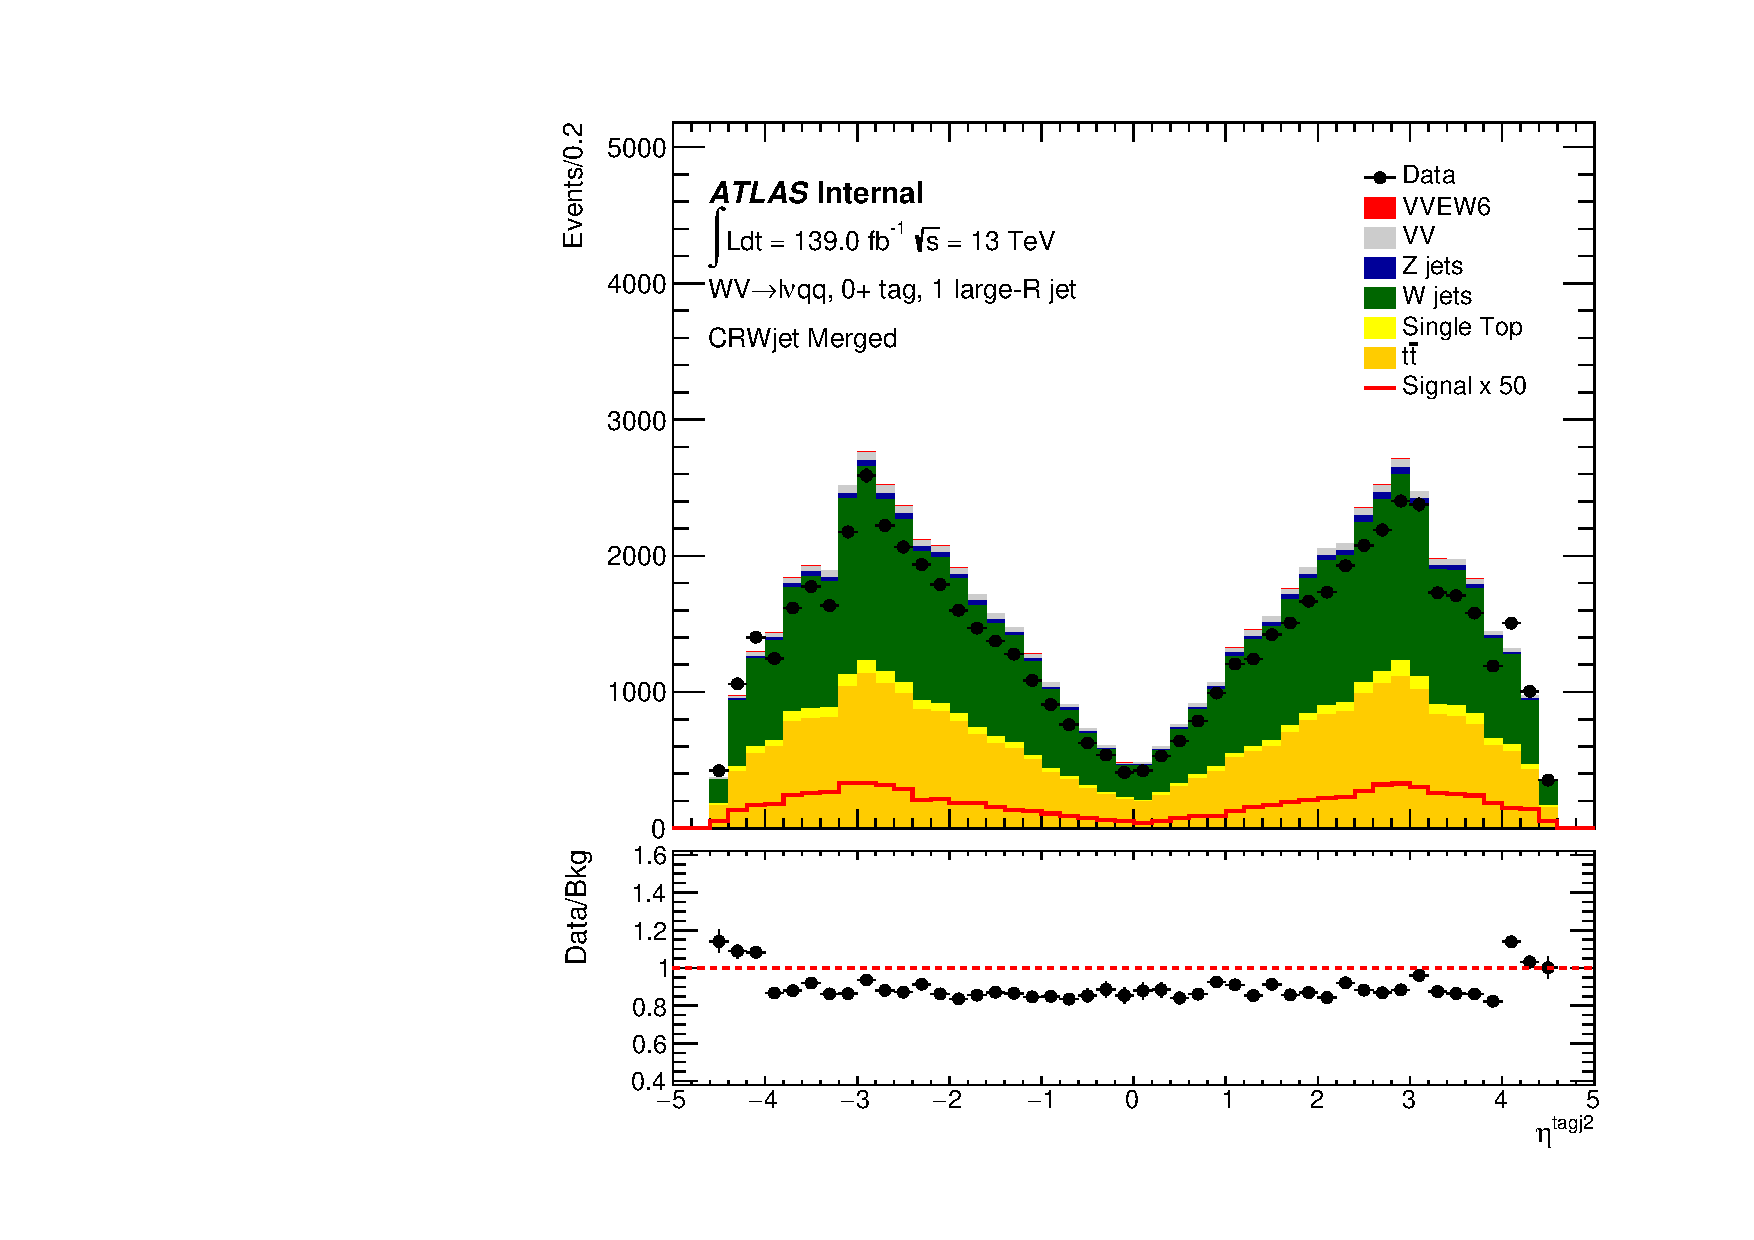
\includegraphics[width=0.3\textwidth]{figures/CRPlots/CRWjets100/stacked_plot_merged_tagJ2_eta.pdf}}
    \subfloat[]{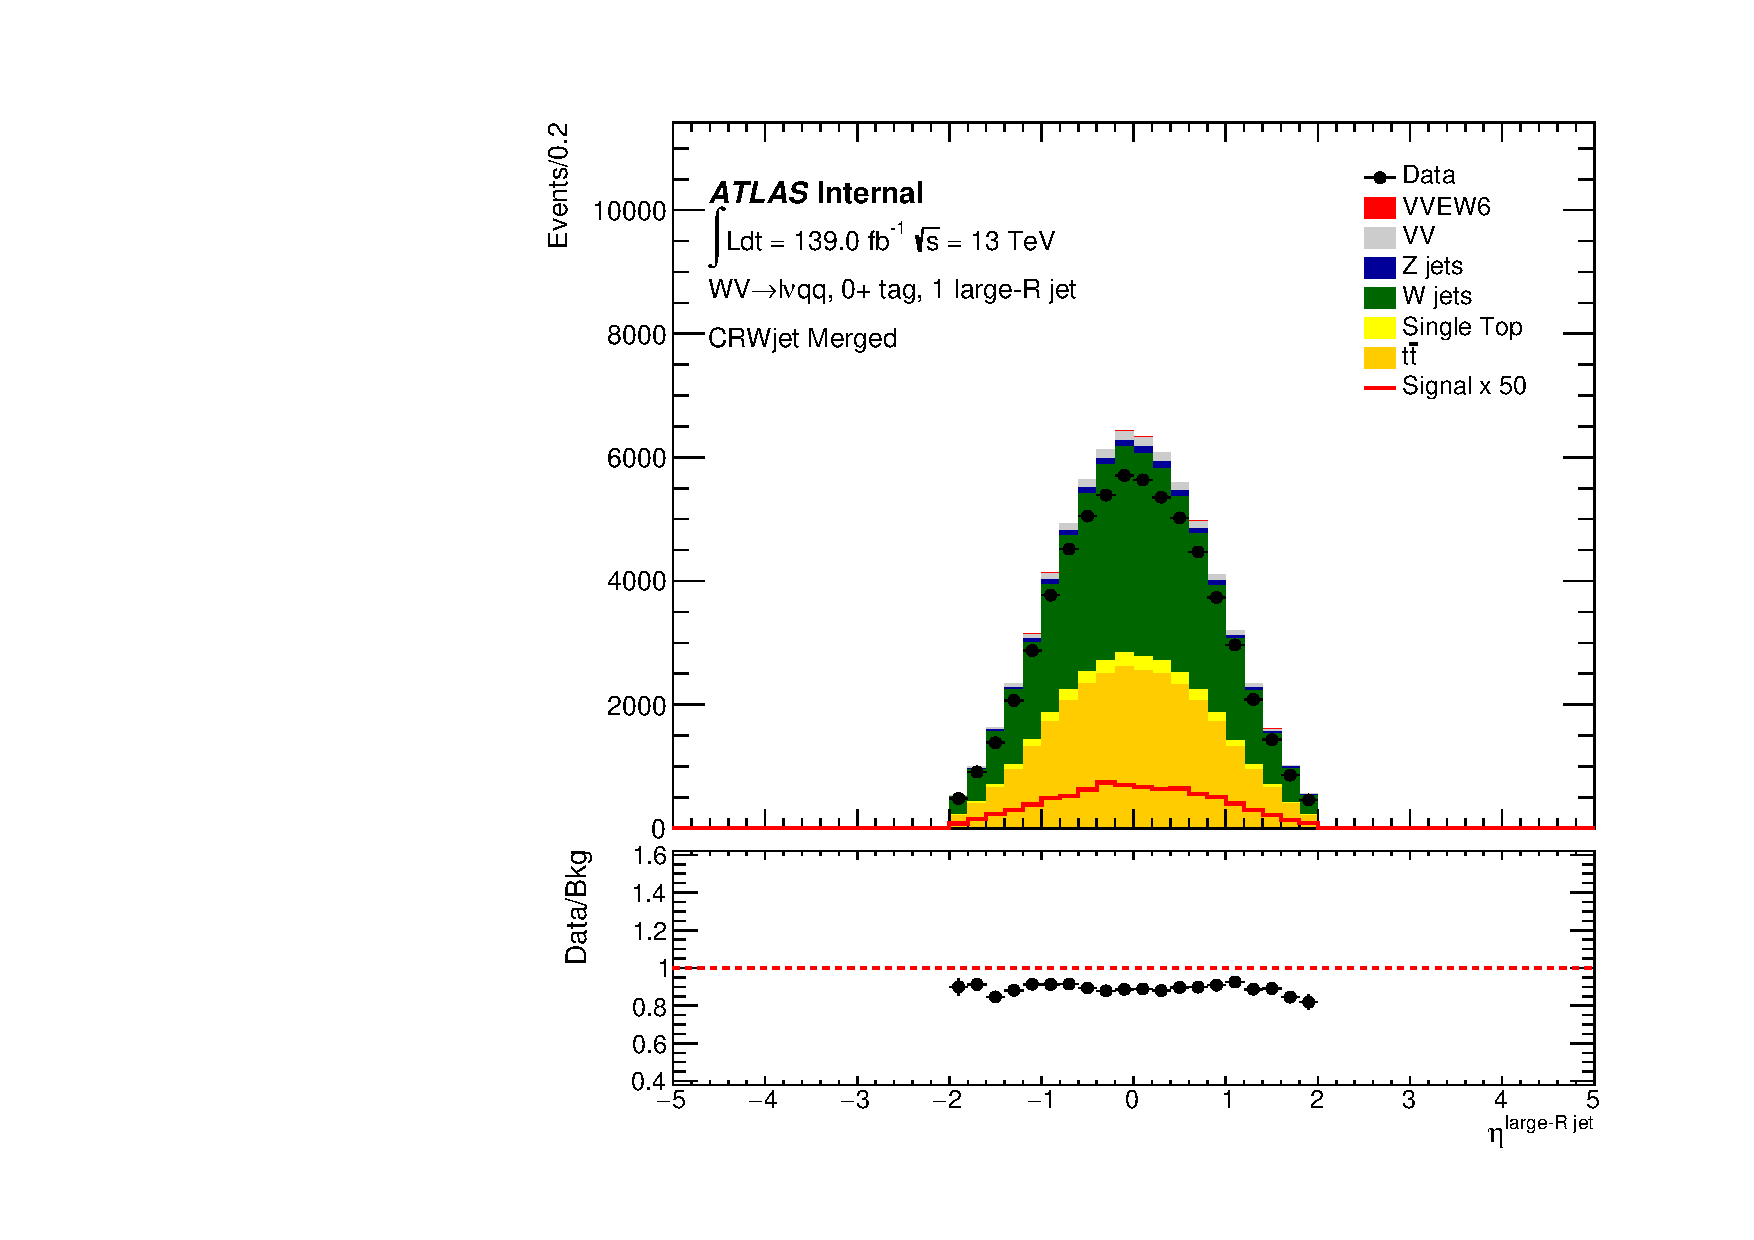
\includegraphics[width=0.3\textwidth]{figures/CRPlots/CRWjets100/stacked_plot_fatJ_eta.pdf}} \\
    \subfloat[]{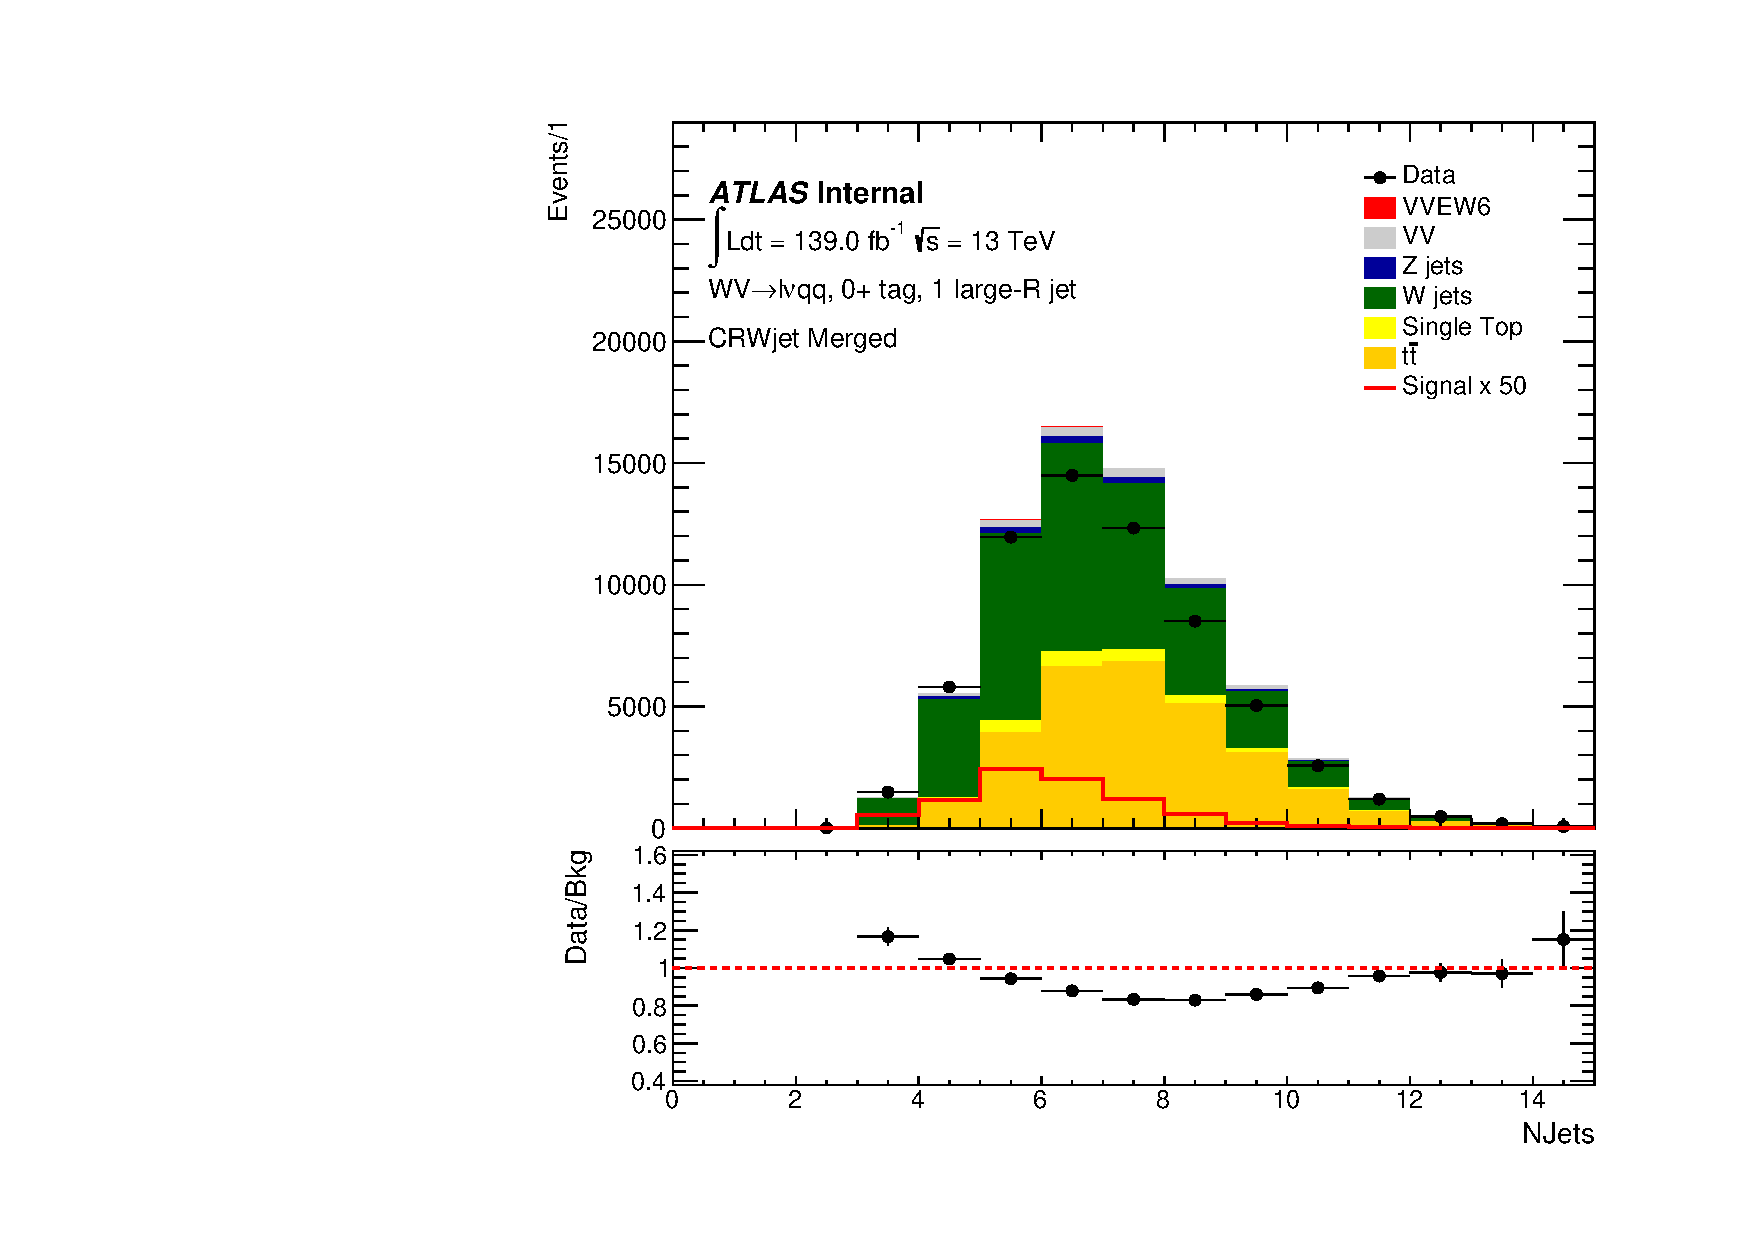
\includegraphics[width=0.3\textwidth]{figures/CRPlots/CRWjets100/stacked_plot_NJets.pdf}}
    \subfloat[]{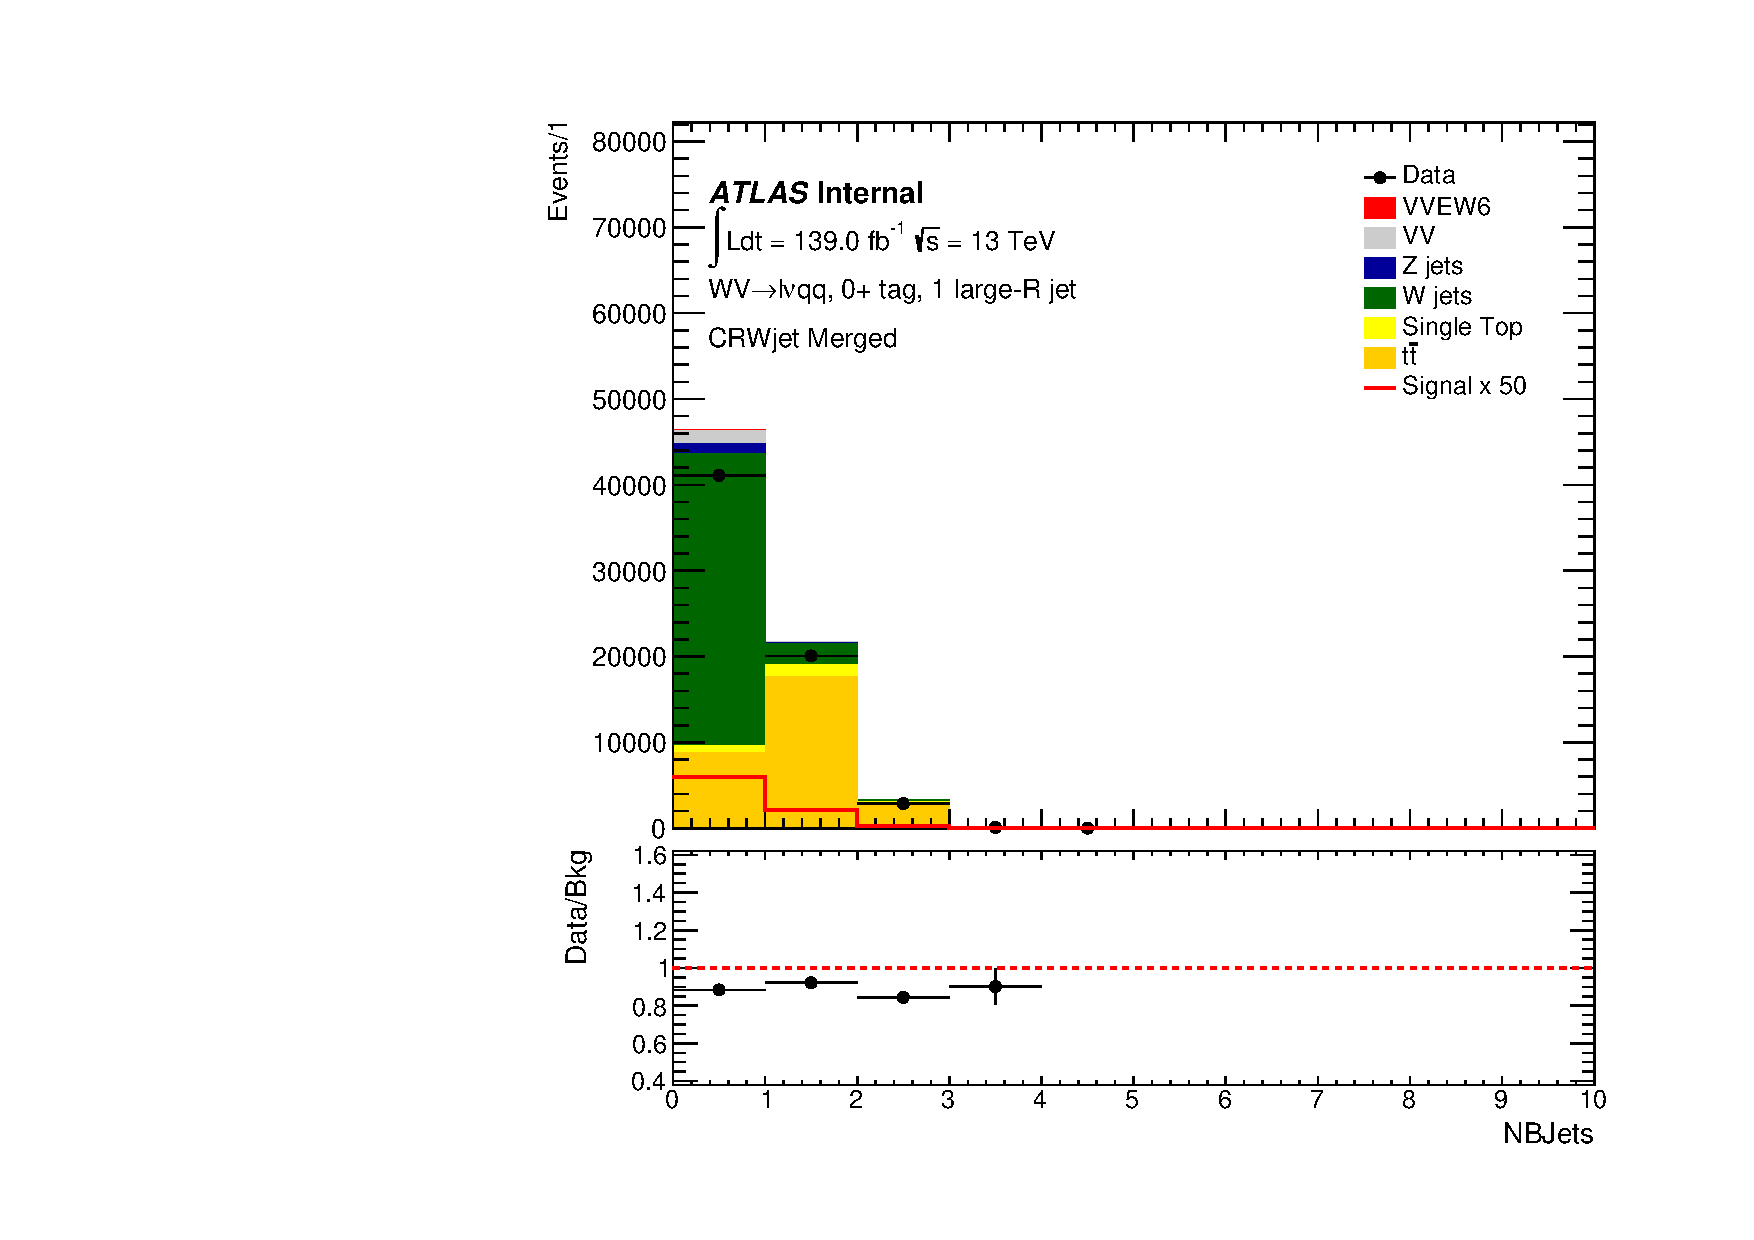
\includegraphics[width=0.3\textwidth]{figures/CRPlots/CRWjets100/stacked_plot_NBJets.pdf}}
    \subfloat[]{\includegraphics[width=0.3\textwidth]{figures/CRPlots/CRWjets100/stacked_plot_lep_pt.pdf}}  \\
    \subfloat[]{\includegraphics[width=0.3\textwidth]{figures/CRPlots/CRWjets100/stacked_plot_fatJ_m.pdf}}
    \subfloat[]{\includegraphics[width=0.3\textwidth]{figures/CRPlots/CRWjets100/stacked_plot_fatJ_pt.pdf}}
    \subfloat[]{\includegraphics[width=0.3\textwidth]{figures/CRPlots/CRWjets100/stacked_plot_fatJ_D2.pdf}}
    \caption{Data-MC checks for the merged \Wjets control region in the \olep channel.}
    \label{fig:CRWjetMerPlots1Lep}
\end{figure}

\begin{figure}[ht]
    \centering
    \subfloat[]{\includegraphics[width=0.3\textwidth]{figures/CRPlots/CRWjets100/stacked_plot_W_m.pdf}}
    \subfloat[]{\includegraphics[width=0.3\textwidth]{figures/CRPlots/CRWjets100/stacked_plot_W_pt.pdf}}
    \subfloat[]{\includegraphics[width=0.3\textwidth]{figures/CRPlots/CRWjets100/stacked_plot_W_eta.pdf}} \\
    \subfloat[]{\includegraphics[width=0.3\textwidth]{figures/CRPlots/CRWjets100/stacked_plot_merged_tagJdEta.pdf}}
    \subfloat[]{\includegraphics[width=0.3\textwidth]{figures/CRPlots/CRWjets100/stacked_plot_fatJ_dRj1.pdf}}
    \subfloat[]{\includegraphics[width=0.3\textwidth]{figures/CRPlots/CRWjets100/stacked_plot_fatJ_dRj2.pdf}} \\
    \subfloat[]{\includegraphics[width=0.3\textwidth]{figures/CRPlots/CRWjets100/stacked_plot_lvJjjmass.pdf}}
    \subfloat[]{\includegraphics[width=0.3\textwidth]{figures/CRPlots/CRWjets100/stacked_plot_lvJmass.pdf}} \\
    \caption{Data-MC checks for the merged \Wjets control region in the \olep channel.}
    \label{fig:CRWjetMerPlots1Lep2}
\end{figure}

%%%

%%\begin{figure}[ht]
%%    \centering
%%    \subfigure[]{\includegraphics[width=0.3\textwidth]{figures/CRPlots/WjetsCR/C_0ptag1pfat0pjet_0ptv_CRVjet_Merged_Mer_tagMjj_Lin.pdf}}
%%    \subfigure[]{\includegraphics[width=0.3\textwidth]{figures/CRPlots/WjetsCR/C_0ptag1pfat0pjet_0ptv_CRVjet_Merged_PtTagMerJet1_Lin.pdf}}
%%    \subfigure[]{\includegraphics[width=0.3\textwidth]{figures/CRPlots/WjetsCR/C_0ptag1pfat0pjet_0ptv_CRVjet_Merged_PtTagMerJet2_Lin.pdf}} \\
%%    \subfigure[]{\includegraphics[width=0.3\textwidth]{figures/CRPlots/WjetsCR/C_0ptag1pfat0pjet_0ptv_CRVjet_Merged_EtaTagMerJet1_Lin.pdf}}
%%    \subfigure[]{\includegraphics[width=0.3\textwidth]{figures/CRPlots/WjetsCR/C_0ptag1pfat0pjet_0ptv_CRVjet_Merged_EtaTagMerJet2_Lin.pdf}}
%%    \subfigure[]{\includegraphics[width=0.3\textwidth]{figures/CRPlots/WjetsCR/C_0ptag1pfat0pjet_0ptv_CRVjet_Merged_EtaFatJet_Lin.pdf}}\\
%%    \subfigure[]{\includegraphics[width=0.3\textwidth]{figures/CRPlots/WjetsCR/C_0ptag1pfat0pjet_0ptv_CRVjet_Merged_NJets_Lin.pdf}}
%%    \subfigure[]{\includegraphics[width=0.3\textwidth]{figures/CRPlots/WjetsCR/C_0ptag1pfat0pjet_0ptv_CRVjet_Merged_NBJets_Lin.pdf}}
%%    \subfigure[]{\includegraphics[width=0.3\textwidth]{figures/CRPlots/WjetsCR/C_0ptag1pfat0pjet_0ptv_CRVjet_Merged_PtL_Lin.pdf}} \\
%%    \subfigure[]{\includegraphics[width=0.3\textwidth]{figures/CRPlots/WjetsCR/C_0ptag1pfat0pjet_0ptv_CRVjet_Merged_MFatJet_Lin.pdf}}
%%    \subfigure[]{\includegraphics[width=0.3\textwidth]{figures/CRPlots/WjetsCR/C_0ptag1pfat0pjet_0ptv_CRVjet_Merged_PtFatJet_Lin.pdf}}
%%    \subfigure[]{\includegraphics[width=0.3\textwidth]{figures/CRPlots/WjetsCR/C_0ptag1pfat0pjet_0ptv_CRVjet_Merged_D2FatJet_Lin.pdf}}
%%    \caption{Data-MC checks for the merged \Wjets control region in the \olep channel, after \mjjtag reweighting has been applied.}
%%    \label{fig:CRVjetMerPlots1Lep}
%%\end{figure}
%%
%%\begin{figure}[ht]
%%    \centering
%%    \subfigure[]{\includegraphics[width=0.3\textwidth]{figures/CRPlots/WjetsCR/C_0ptag1pfat0pjet_0ptv_CRVjet_Merged_MW_Lin.pdf}}
%%    \subfigure[]{\includegraphics[width=0.3\textwidth]{figures/CRPlots/WjetsCR/C_0ptag1pfat0pjet_0ptv_CRVjet_Merged_PtW_Lin.pdf}}
%%    \subfigure[]{\includegraphics[width=0.3\textwidth]{figures/CRPlots/WjetsCR/C_0ptag1pfat0pjet_0ptv_CRVjet_Merged_EtaW_Lin.pdf}} \\
%%    \subfigure[]{\includegraphics[width=0.3\textwidth]{figures/CRPlots/WjetsCR/C_0ptag1pfat0pjet_0ptv_CRVjet_Merged_DPhiTagMerJet_Lin.pdf}}
%%    \subfigure[]{\includegraphics[width=0.3\textwidth]{figures/CRPlots/WjetsCR/C_0ptag1pfat0pjet_0ptv_CRVjet_Merged_DEtaTagMerJet_Lin.pdf}} \\
%%    \subfigure[]{\includegraphics[width=0.3\textwidth]{figures/CRPlots/WjetsCR/C_0ptag1pfat0pjet_0ptv_CRVjet_Merged_DRFatJetTagJet1_Lin.pdf}}
%%    \subfigure[]{\includegraphics[width=0.3\textwidth]{figures/CRPlots/WjetsCR/C_0ptag1pfat0pjet_0ptv_CRVjet_Merged_DRFatJetTagJet2_Lin.pdf}}
%%    \subfigure[]{\includegraphics[width=0.3\textwidth]{figures/CRPlots/WjetsCR/C_0ptag1pfat0pjet_0ptv_CRVjet_Merged_DRFatJetTagjj_Lin.pdf}}
%%
%%    \caption{Data-MC checks for the merged \Wjets control region in the \olep channel, after \mjjtag reweighting has been applied.}
%%    \label{fig:CRVjetMerPlots1Lep2}
%%\end{figure}

%%\begin{figure}[ht]
%%    \centering
%%    \subfigure[]{\includegraphics[width=0.3\textwidth]{figures/CRPlots/WjetsCR/C_0ptag2pjet_0ptv_CRVjet_Res_tagMjj_Lin.pdf}}
%%    \subfigure[]{\includegraphics[width=0.3\textwidth]{figures/CRPlots/WjetsCR/C_0ptag2pjet_0ptv_CRVjet_PtTagResJet1_Lin.pdf}}
%%    \subfigure[]{\includegraphics[width=0.3\textwidth]{figures/CRPlots/WjetsCR/C_0ptag2pjet_0ptv_CRVjet_PtTagResJet2_Lin.pdf}} \\
%%    \subfigure[]{\includegraphics[width=0.3\textwidth]{figures/CRPlots/WjetsCR/C_0ptag2pjet_0ptv_CRVjet_EtaTagResJet1_Lin.pdf}}
%%    \subfigure[]{\includegraphics[width=0.3\textwidth]{figures/CRPlots/WjetsCR/C_0ptag2pjet_0ptv_CRVjet_EtaTagResJet2_Lin.pdf}} \\
%%    \subfigure[]{\includegraphics[width=0.3\textwidth]{figures/CRPlots/WjetsCR/C_0ptag2pjet_0ptv_CRVjet_NJets_Lin.pdf}}
%%    \subfigure[]{\includegraphics[width=0.3\textwidth]{figures/CRPlots/WjetsCR/C_0ptag2pjet_0ptv_CRVjet_NBJets_Lin.pdf}}
%%    \subfigure[]{\includegraphics[width=0.3\textwidth]{figures/CRPlots/WjetsCR/C_0ptag2pjet_0ptv_CRVjet_PtL_Lin.pdf}}  \\
%%    \subfigure[]{\includegraphics[width=0.3\textwidth]{figures/CRPlots/WjetsCR/C_0ptag2pjet_0ptv_CRVjet_MW_Lin.pdf}}
%%    \subfigure[]{\includegraphics[width=0.3\textwidth]{figures/CRPlots/WjetsCR/C_0ptag2pjet_0ptv_CRVjet_PtW_Lin.pdf}}
%%    \subfigure[]{\includegraphics[width=0.3\textwidth]{figures/CRPlots/WjetsCR/C_0ptag2pjet_0ptv_CRVjet_EtaW_Lin.pdf}}
%%    \caption{Data-MC checks for the resolved loose \Wjets control region in the \olep channel, after \mjjtag reweighting has been applied.}
%%    \label{fig:CRVjetResLoosePlots1Lep}
%%\end{figure}
%%
%%\begin{figure}[ht]
%%    \centering
%%    \subfigure[]{\includegraphics[width=0.3\textwidth]{figures/CRPlots/WjetsCR/C_0ptag2pjet_0ptv_CRVjet_DPhiTagResJet_Lin.pdf}}
%%    \subfigure[]{\includegraphics[width=0.3\textwidth]{figures/CRPlots/WjetsCR/C_0ptag2pjet_0ptv_CRVjet_DEtaTagResJet_Lin.pdf}} \\
%%    \subfigure[]{\includegraphics[width=0.3\textwidth]{figures/CRPlots/WjetsCR/C_0ptag2pjet_0ptv_CRVjet_DRSigjjTagJet1_Lin.pdf}}
%%    \subfigure[]{\includegraphics[width=0.3\textwidth]{figures/CRPlots/WjetsCR/C_0ptag2pjet_0ptv_CRVjet_DRSigjjTagJet2_Lin.pdf}}
%%    \subfigure[]{\includegraphics[width=0.3\textwidth]{figures/CRPlots/WjetsCR/C_0ptag2pjet_0ptv_CRVjet_DRSigjjTagjj_Lin.pdf}} \\
%%    \subfigure[]{\includegraphics[width=0.3\textwidth]{figures/CRPlots/WjetsCR/C_0ptag2pjet_0ptv_CRVjet_EtaSigJet1_Lin.pdf}}
%%    \subfigure[]{\includegraphics[width=0.3\textwidth]{figures/CRPlots/WjetsCR/C_0ptag2pjet_0ptv_CRVjet_EtaSigJet2_Lin.pdf}}
%%    \caption{Data-MC checks for the resolved loose \Wjets control region in the \olep channel, after \mjjtag reweighting has been applied.}
%%    \label{fig:CRVjetResLoosePlots1Lep2}
%%\end{figure}

